\documentclass[11pt]{article}

    \usepackage[breakable]{tcolorbox}
    \usepackage{parskip} % Stop auto-indenting (to mimic markdown behaviour)
    
    \usepackage{iftex}
    \ifPDFTeX
    	\usepackage[T1]{fontenc}
    	\usepackage{mathpazo}
    \else
    	\usepackage{fontspec}
    \fi

    % Basic figure setup, for now with no caption control since it's done
    % automatically by Pandoc (which extracts ![](path) syntax from Markdown).
    \usepackage{graphicx}
    % Maintain compatibility with old templates. Remove in nbconvert 6.0
    \let\Oldincludegraphics\includegraphics
    % Ensure that by default, figures have no caption (until we provide a
    % proper Figure object with a Caption API and a way to capture that
    % in the conversion process - todo).
    \usepackage{caption}
    \DeclareCaptionFormat{nocaption}{}
    \captionsetup{format=nocaption,aboveskip=0pt,belowskip=0pt}

    \usepackage{float}
    \floatplacement{figure}{H} % forces figures to be placed at the correct location
    \usepackage{xcolor} % Allow colors to be defined
    \usepackage{enumerate} % Needed for markdown enumerations to work
    \usepackage{geometry} % Used to adjust the document margins
    \usepackage{amsmath} % Equations
    \usepackage{amssymb} % Equations
    \usepackage{textcomp} % defines textquotesingle
    % Hack from http://tex.stackexchange.com/a/47451/13684:
    \AtBeginDocument{%
        \def\PYZsq{\textquotesingle}% Upright quotes in Pygmentized code
    }
    \usepackage{upquote} % Upright quotes for verbatim code
    \usepackage{eurosym} % defines \euro
    \usepackage[mathletters]{ucs} % Extended unicode (utf-8) support
    \usepackage{fancyvrb} % verbatim replacement that allows latex
    \usepackage{grffile} % extends the file name processing of package graphics 
                         % to support a larger range
    \makeatletter % fix for old versions of grffile with XeLaTeX
    \@ifpackagelater{grffile}{2019/11/01}
    {
      % Do nothing on new versions
    }
    {
      \def\Gread@@xetex#1{%
        \IfFileExists{"\Gin@base".bb}%
        {\Gread@eps{\Gin@base.bb}}%
        {\Gread@@xetex@aux#1}%
      }
    }
    \makeatother
    \usepackage[Export]{adjustbox} % Used to constrain images to a maximum size
    \adjustboxset{max size={0.9\linewidth}{0.9\paperheight}}

    % The hyperref package gives us a pdf with properly built
    % internal navigation ('pdf bookmarks' for the table of contents,
    % internal cross-reference links, web links for URLs, etc.)
    \usepackage{hyperref}
    % The default LaTeX title has an obnoxious amount of whitespace. By default,
    % titling removes some of it. It also provides customization options.
    \usepackage{titling}
    \usepackage{longtable} % longtable support required by pandoc >1.10
    \usepackage{booktabs}  % table support for pandoc > 1.12.2
    \usepackage[inline]{enumitem} % IRkernel/repr support (it uses the enumerate* environment)
    \usepackage[normalem]{ulem} % ulem is needed to support strikethroughs (\sout)
                                % normalem makes italics be italics, not underlines
    \usepackage{mathrsfs}
    

    
    % Colors for the hyperref package
    \definecolor{urlcolor}{rgb}{0,.145,.698}
    \definecolor{linkcolor}{rgb}{.71,0.21,0.01}
    \definecolor{citecolor}{rgb}{.12,.54,.11}

    % ANSI colors
    \definecolor{ansi-black}{HTML}{3E424D}
    \definecolor{ansi-black-intense}{HTML}{282C36}
    \definecolor{ansi-red}{HTML}{E75C58}
    \definecolor{ansi-red-intense}{HTML}{B22B31}
    \definecolor{ansi-green}{HTML}{00A250}
    \definecolor{ansi-green-intense}{HTML}{007427}
    \definecolor{ansi-yellow}{HTML}{DDB62B}
    \definecolor{ansi-yellow-intense}{HTML}{B27D12}
    \definecolor{ansi-blue}{HTML}{208FFB}
    \definecolor{ansi-blue-intense}{HTML}{0065CA}
    \definecolor{ansi-magenta}{HTML}{D160C4}
    \definecolor{ansi-magenta-intense}{HTML}{A03196}
    \definecolor{ansi-cyan}{HTML}{60C6C8}
    \definecolor{ansi-cyan-intense}{HTML}{258F8F}
    \definecolor{ansi-white}{HTML}{C5C1B4}
    \definecolor{ansi-white-intense}{HTML}{A1A6B2}
    \definecolor{ansi-default-inverse-fg}{HTML}{FFFFFF}
    \definecolor{ansi-default-inverse-bg}{HTML}{000000}

    % common color for the border for error outputs.
    \definecolor{outerrorbackground}{HTML}{FFDFDF}

    % commands and environments needed by pandoc snippets
    % extracted from the output of `pandoc -s`
    \providecommand{\tightlist}{%
      \setlength{\itemsep}{0pt}\setlength{\parskip}{0pt}}
    \DefineVerbatimEnvironment{Highlighting}{Verbatim}{commandchars=\\\{\}}
    % Add ',fontsize=\small' for more characters per line
    \newenvironment{Shaded}{}{}
    \newcommand{\KeywordTok}[1]{\textcolor[rgb]{0.00,0.44,0.13}{\textbf{{#1}}}}
    \newcommand{\DataTypeTok}[1]{\textcolor[rgb]{0.56,0.13,0.00}{{#1}}}
    \newcommand{\DecValTok}[1]{\textcolor[rgb]{0.25,0.63,0.44}{{#1}}}
    \newcommand{\BaseNTok}[1]{\textcolor[rgb]{0.25,0.63,0.44}{{#1}}}
    \newcommand{\FloatTok}[1]{\textcolor[rgb]{0.25,0.63,0.44}{{#1}}}
    \newcommand{\CharTok}[1]{\textcolor[rgb]{0.25,0.44,0.63}{{#1}}}
    \newcommand{\StringTok}[1]{\textcolor[rgb]{0.25,0.44,0.63}{{#1}}}
    \newcommand{\CommentTok}[1]{\textcolor[rgb]{0.38,0.63,0.69}{\textit{{#1}}}}
    \newcommand{\OtherTok}[1]{\textcolor[rgb]{0.00,0.44,0.13}{{#1}}}
    \newcommand{\AlertTok}[1]{\textcolor[rgb]{1.00,0.00,0.00}{\textbf{{#1}}}}
    \newcommand{\FunctionTok}[1]{\textcolor[rgb]{0.02,0.16,0.49}{{#1}}}
    \newcommand{\RegionMarkerTok}[1]{{#1}}
    \newcommand{\ErrorTok}[1]{\textcolor[rgb]{1.00,0.00,0.00}{\textbf{{#1}}}}
    \newcommand{\NormalTok}[1]{{#1}}
    
    % Additional commands for more recent versions of Pandoc
    \newcommand{\ConstantTok}[1]{\textcolor[rgb]{0.53,0.00,0.00}{{#1}}}
    \newcommand{\SpecialCharTok}[1]{\textcolor[rgb]{0.25,0.44,0.63}{{#1}}}
    \newcommand{\VerbatimStringTok}[1]{\textcolor[rgb]{0.25,0.44,0.63}{{#1}}}
    \newcommand{\SpecialStringTok}[1]{\textcolor[rgb]{0.73,0.40,0.53}{{#1}}}
    \newcommand{\ImportTok}[1]{{#1}}
    \newcommand{\DocumentationTok}[1]{\textcolor[rgb]{0.73,0.13,0.13}{\textit{{#1}}}}
    \newcommand{\AnnotationTok}[1]{\textcolor[rgb]{0.38,0.63,0.69}{\textbf{\textit{{#1}}}}}
    \newcommand{\CommentVarTok}[1]{\textcolor[rgb]{0.38,0.63,0.69}{\textbf{\textit{{#1}}}}}
    \newcommand{\VariableTok}[1]{\textcolor[rgb]{0.10,0.09,0.49}{{#1}}}
    \newcommand{\ControlFlowTok}[1]{\textcolor[rgb]{0.00,0.44,0.13}{\textbf{{#1}}}}
    \newcommand{\OperatorTok}[1]{\textcolor[rgb]{0.40,0.40,0.40}{{#1}}}
    \newcommand{\BuiltInTok}[1]{{#1}}
    \newcommand{\ExtensionTok}[1]{{#1}}
    \newcommand{\PreprocessorTok}[1]{\textcolor[rgb]{0.74,0.48,0.00}{{#1}}}
    \newcommand{\AttributeTok}[1]{\textcolor[rgb]{0.49,0.56,0.16}{{#1}}}
    \newcommand{\InformationTok}[1]{\textcolor[rgb]{0.38,0.63,0.69}{\textbf{\textit{{#1}}}}}
    \newcommand{\WarningTok}[1]{\textcolor[rgb]{0.38,0.63,0.69}{\textbf{\textit{{#1}}}}}
    
    
    % Define a nice break command that doesn't care if a line doesn't already
    % exist.
    \def\br{\hspace*{\fill} \\* }
    % Math Jax compatibility definitions
    \def\gt{>}
    \def\lt{<}
    \let\Oldtex\TeX
    \let\Oldlatex\LaTeX
    \renewcommand{\TeX}{\textrm{\Oldtex}}
    \renewcommand{\LaTeX}{\textrm{\Oldlatex}}
    % Document parameters
    % Document title
    \title{Brady}
    
    
    
    
    
% Pygments definitions
\makeatletter
\def\PY@reset{\let\PY@it=\relax \let\PY@bf=\relax%
    \let\PY@ul=\relax \let\PY@tc=\relax%
    \let\PY@bc=\relax \let\PY@ff=\relax}
\def\PY@tok#1{\csname PY@tok@#1\endcsname}
\def\PY@toks#1+{\ifx\relax#1\empty\else%
    \PY@tok{#1}\expandafter\PY@toks\fi}
\def\PY@do#1{\PY@bc{\PY@tc{\PY@ul{%
    \PY@it{\PY@bf{\PY@ff{#1}}}}}}}
\def\PY#1#2{\PY@reset\PY@toks#1+\relax+\PY@do{#2}}

\@namedef{PY@tok@w}{\def\PY@tc##1{\textcolor[rgb]{0.73,0.73,0.73}{##1}}}
\@namedef{PY@tok@c}{\let\PY@it=\textit\def\PY@tc##1{\textcolor[rgb]{0.25,0.50,0.50}{##1}}}
\@namedef{PY@tok@cp}{\def\PY@tc##1{\textcolor[rgb]{0.74,0.48,0.00}{##1}}}
\@namedef{PY@tok@k}{\let\PY@bf=\textbf\def\PY@tc##1{\textcolor[rgb]{0.00,0.50,0.00}{##1}}}
\@namedef{PY@tok@kp}{\def\PY@tc##1{\textcolor[rgb]{0.00,0.50,0.00}{##1}}}
\@namedef{PY@tok@kt}{\def\PY@tc##1{\textcolor[rgb]{0.69,0.00,0.25}{##1}}}
\@namedef{PY@tok@o}{\def\PY@tc##1{\textcolor[rgb]{0.40,0.40,0.40}{##1}}}
\@namedef{PY@tok@ow}{\let\PY@bf=\textbf\def\PY@tc##1{\textcolor[rgb]{0.67,0.13,1.00}{##1}}}
\@namedef{PY@tok@nb}{\def\PY@tc##1{\textcolor[rgb]{0.00,0.50,0.00}{##1}}}
\@namedef{PY@tok@nf}{\def\PY@tc##1{\textcolor[rgb]{0.00,0.00,1.00}{##1}}}
\@namedef{PY@tok@nc}{\let\PY@bf=\textbf\def\PY@tc##1{\textcolor[rgb]{0.00,0.00,1.00}{##1}}}
\@namedef{PY@tok@nn}{\let\PY@bf=\textbf\def\PY@tc##1{\textcolor[rgb]{0.00,0.00,1.00}{##1}}}
\@namedef{PY@tok@ne}{\let\PY@bf=\textbf\def\PY@tc##1{\textcolor[rgb]{0.82,0.25,0.23}{##1}}}
\@namedef{PY@tok@nv}{\def\PY@tc##1{\textcolor[rgb]{0.10,0.09,0.49}{##1}}}
\@namedef{PY@tok@no}{\def\PY@tc##1{\textcolor[rgb]{0.53,0.00,0.00}{##1}}}
\@namedef{PY@tok@nl}{\def\PY@tc##1{\textcolor[rgb]{0.63,0.63,0.00}{##1}}}
\@namedef{PY@tok@ni}{\let\PY@bf=\textbf\def\PY@tc##1{\textcolor[rgb]{0.60,0.60,0.60}{##1}}}
\@namedef{PY@tok@na}{\def\PY@tc##1{\textcolor[rgb]{0.49,0.56,0.16}{##1}}}
\@namedef{PY@tok@nt}{\let\PY@bf=\textbf\def\PY@tc##1{\textcolor[rgb]{0.00,0.50,0.00}{##1}}}
\@namedef{PY@tok@nd}{\def\PY@tc##1{\textcolor[rgb]{0.67,0.13,1.00}{##1}}}
\@namedef{PY@tok@s}{\def\PY@tc##1{\textcolor[rgb]{0.73,0.13,0.13}{##1}}}
\@namedef{PY@tok@sd}{\let\PY@it=\textit\def\PY@tc##1{\textcolor[rgb]{0.73,0.13,0.13}{##1}}}
\@namedef{PY@tok@si}{\let\PY@bf=\textbf\def\PY@tc##1{\textcolor[rgb]{0.73,0.40,0.53}{##1}}}
\@namedef{PY@tok@se}{\let\PY@bf=\textbf\def\PY@tc##1{\textcolor[rgb]{0.73,0.40,0.13}{##1}}}
\@namedef{PY@tok@sr}{\def\PY@tc##1{\textcolor[rgb]{0.73,0.40,0.53}{##1}}}
\@namedef{PY@tok@ss}{\def\PY@tc##1{\textcolor[rgb]{0.10,0.09,0.49}{##1}}}
\@namedef{PY@tok@sx}{\def\PY@tc##1{\textcolor[rgb]{0.00,0.50,0.00}{##1}}}
\@namedef{PY@tok@m}{\def\PY@tc##1{\textcolor[rgb]{0.40,0.40,0.40}{##1}}}
\@namedef{PY@tok@gh}{\let\PY@bf=\textbf\def\PY@tc##1{\textcolor[rgb]{0.00,0.00,0.50}{##1}}}
\@namedef{PY@tok@gu}{\let\PY@bf=\textbf\def\PY@tc##1{\textcolor[rgb]{0.50,0.00,0.50}{##1}}}
\@namedef{PY@tok@gd}{\def\PY@tc##1{\textcolor[rgb]{0.63,0.00,0.00}{##1}}}
\@namedef{PY@tok@gi}{\def\PY@tc##1{\textcolor[rgb]{0.00,0.63,0.00}{##1}}}
\@namedef{PY@tok@gr}{\def\PY@tc##1{\textcolor[rgb]{1.00,0.00,0.00}{##1}}}
\@namedef{PY@tok@ge}{\let\PY@it=\textit}
\@namedef{PY@tok@gs}{\let\PY@bf=\textbf}
\@namedef{PY@tok@gp}{\let\PY@bf=\textbf\def\PY@tc##1{\textcolor[rgb]{0.00,0.00,0.50}{##1}}}
\@namedef{PY@tok@go}{\def\PY@tc##1{\textcolor[rgb]{0.53,0.53,0.53}{##1}}}
\@namedef{PY@tok@gt}{\def\PY@tc##1{\textcolor[rgb]{0.00,0.27,0.87}{##1}}}
\@namedef{PY@tok@err}{\def\PY@bc##1{{\setlength{\fboxsep}{-\fboxrule}\fcolorbox[rgb]{1.00,0.00,0.00}{1,1,1}{\strut ##1}}}}
\@namedef{PY@tok@kc}{\let\PY@bf=\textbf\def\PY@tc##1{\textcolor[rgb]{0.00,0.50,0.00}{##1}}}
\@namedef{PY@tok@kd}{\let\PY@bf=\textbf\def\PY@tc##1{\textcolor[rgb]{0.00,0.50,0.00}{##1}}}
\@namedef{PY@tok@kn}{\let\PY@bf=\textbf\def\PY@tc##1{\textcolor[rgb]{0.00,0.50,0.00}{##1}}}
\@namedef{PY@tok@kr}{\let\PY@bf=\textbf\def\PY@tc##1{\textcolor[rgb]{0.00,0.50,0.00}{##1}}}
\@namedef{PY@tok@bp}{\def\PY@tc##1{\textcolor[rgb]{0.00,0.50,0.00}{##1}}}
\@namedef{PY@tok@fm}{\def\PY@tc##1{\textcolor[rgb]{0.00,0.00,1.00}{##1}}}
\@namedef{PY@tok@vc}{\def\PY@tc##1{\textcolor[rgb]{0.10,0.09,0.49}{##1}}}
\@namedef{PY@tok@vg}{\def\PY@tc##1{\textcolor[rgb]{0.10,0.09,0.49}{##1}}}
\@namedef{PY@tok@vi}{\def\PY@tc##1{\textcolor[rgb]{0.10,0.09,0.49}{##1}}}
\@namedef{PY@tok@vm}{\def\PY@tc##1{\textcolor[rgb]{0.10,0.09,0.49}{##1}}}
\@namedef{PY@tok@sa}{\def\PY@tc##1{\textcolor[rgb]{0.73,0.13,0.13}{##1}}}
\@namedef{PY@tok@sb}{\def\PY@tc##1{\textcolor[rgb]{0.73,0.13,0.13}{##1}}}
\@namedef{PY@tok@sc}{\def\PY@tc##1{\textcolor[rgb]{0.73,0.13,0.13}{##1}}}
\@namedef{PY@tok@dl}{\def\PY@tc##1{\textcolor[rgb]{0.73,0.13,0.13}{##1}}}
\@namedef{PY@tok@s2}{\def\PY@tc##1{\textcolor[rgb]{0.73,0.13,0.13}{##1}}}
\@namedef{PY@tok@sh}{\def\PY@tc##1{\textcolor[rgb]{0.73,0.13,0.13}{##1}}}
\@namedef{PY@tok@s1}{\def\PY@tc##1{\textcolor[rgb]{0.73,0.13,0.13}{##1}}}
\@namedef{PY@tok@mb}{\def\PY@tc##1{\textcolor[rgb]{0.40,0.40,0.40}{##1}}}
\@namedef{PY@tok@mf}{\def\PY@tc##1{\textcolor[rgb]{0.40,0.40,0.40}{##1}}}
\@namedef{PY@tok@mh}{\def\PY@tc##1{\textcolor[rgb]{0.40,0.40,0.40}{##1}}}
\@namedef{PY@tok@mi}{\def\PY@tc##1{\textcolor[rgb]{0.40,0.40,0.40}{##1}}}
\@namedef{PY@tok@il}{\def\PY@tc##1{\textcolor[rgb]{0.40,0.40,0.40}{##1}}}
\@namedef{PY@tok@mo}{\def\PY@tc##1{\textcolor[rgb]{0.40,0.40,0.40}{##1}}}
\@namedef{PY@tok@ch}{\let\PY@it=\textit\def\PY@tc##1{\textcolor[rgb]{0.25,0.50,0.50}{##1}}}
\@namedef{PY@tok@cm}{\let\PY@it=\textit\def\PY@tc##1{\textcolor[rgb]{0.25,0.50,0.50}{##1}}}
\@namedef{PY@tok@cpf}{\let\PY@it=\textit\def\PY@tc##1{\textcolor[rgb]{0.25,0.50,0.50}{##1}}}
\@namedef{PY@tok@c1}{\let\PY@it=\textit\def\PY@tc##1{\textcolor[rgb]{0.25,0.50,0.50}{##1}}}
\@namedef{PY@tok@cs}{\let\PY@it=\textit\def\PY@tc##1{\textcolor[rgb]{0.25,0.50,0.50}{##1}}}

\def\PYZbs{\char`\\}
\def\PYZus{\char`\_}
\def\PYZob{\char`\{}
\def\PYZcb{\char`\}}
\def\PYZca{\char`\^}
\def\PYZam{\char`\&}
\def\PYZlt{\char`\<}
\def\PYZgt{\char`\>}
\def\PYZsh{\char`\#}
\def\PYZpc{\char`\%}
\def\PYZdl{\char`\$}
\def\PYZhy{\char`\-}
\def\PYZsq{\char`\'}
\def\PYZdq{\char`\"}
\def\PYZti{\char`\~}
% for compatibility with earlier versions
\def\PYZat{@}
\def\PYZlb{[}
\def\PYZrb{]}
\makeatother


    % For linebreaks inside Verbatim environment from package fancyvrb. 
    \makeatletter
        \newbox\Wrappedcontinuationbox 
        \newbox\Wrappedvisiblespacebox 
        \newcommand*\Wrappedvisiblespace {\textcolor{red}{\textvisiblespace}} 
        \newcommand*\Wrappedcontinuationsymbol {\textcolor{red}{\llap{\tiny$\m@th\hookrightarrow$}}} 
        \newcommand*\Wrappedcontinuationindent {3ex } 
        \newcommand*\Wrappedafterbreak {\kern\Wrappedcontinuationindent\copy\Wrappedcontinuationbox} 
        % Take advantage of the already applied Pygments mark-up to insert 
        % potential linebreaks for TeX processing. 
        %        {, <, #, %, $, ' and ": go to next line. 
        %        _, }, ^, &, >, - and ~: stay at end of broken line. 
        % Use of \textquotesingle for straight quote. 
        \newcommand*\Wrappedbreaksatspecials {% 
            \def\PYGZus{\discretionary{\char`\_}{\Wrappedafterbreak}{\char`\_}}% 
            \def\PYGZob{\discretionary{}{\Wrappedafterbreak\char`\{}{\char`\{}}% 
            \def\PYGZcb{\discretionary{\char`\}}{\Wrappedafterbreak}{\char`\}}}% 
            \def\PYGZca{\discretionary{\char`\^}{\Wrappedafterbreak}{\char`\^}}% 
            \def\PYGZam{\discretionary{\char`\&}{\Wrappedafterbreak}{\char`\&}}% 
            \def\PYGZlt{\discretionary{}{\Wrappedafterbreak\char`\<}{\char`\<}}% 
            \def\PYGZgt{\discretionary{\char`\>}{\Wrappedafterbreak}{\char`\>}}% 
            \def\PYGZsh{\discretionary{}{\Wrappedafterbreak\char`\#}{\char`\#}}% 
            \def\PYGZpc{\discretionary{}{\Wrappedafterbreak\char`\%}{\char`\%}}% 
            \def\PYGZdl{\discretionary{}{\Wrappedafterbreak\char`\$}{\char`\$}}% 
            \def\PYGZhy{\discretionary{\char`\-}{\Wrappedafterbreak}{\char`\-}}% 
            \def\PYGZsq{\discretionary{}{\Wrappedafterbreak\textquotesingle}{\textquotesingle}}% 
            \def\PYGZdq{\discretionary{}{\Wrappedafterbreak\char`\"}{\char`\"}}% 
            \def\PYGZti{\discretionary{\char`\~}{\Wrappedafterbreak}{\char`\~}}% 
        } 
        % Some characters . , ; ? ! / are not pygmentized. 
        % This macro makes them "active" and they will insert potential linebreaks 
        \newcommand*\Wrappedbreaksatpunct {% 
            \lccode`\~`\.\lowercase{\def~}{\discretionary{\hbox{\char`\.}}{\Wrappedafterbreak}{\hbox{\char`\.}}}% 
            \lccode`\~`\,\lowercase{\def~}{\discretionary{\hbox{\char`\,}}{\Wrappedafterbreak}{\hbox{\char`\,}}}% 
            \lccode`\~`\;\lowercase{\def~}{\discretionary{\hbox{\char`\;}}{\Wrappedafterbreak}{\hbox{\char`\;}}}% 
            \lccode`\~`\:\lowercase{\def~}{\discretionary{\hbox{\char`\:}}{\Wrappedafterbreak}{\hbox{\char`\:}}}% 
            \lccode`\~`\?\lowercase{\def~}{\discretionary{\hbox{\char`\?}}{\Wrappedafterbreak}{\hbox{\char`\?}}}% 
            \lccode`\~`\!\lowercase{\def~}{\discretionary{\hbox{\char`\!}}{\Wrappedafterbreak}{\hbox{\char`\!}}}% 
            \lccode`\~`\/\lowercase{\def~}{\discretionary{\hbox{\char`\/}}{\Wrappedafterbreak}{\hbox{\char`\/}}}% 
            \catcode`\.\active
            \catcode`\,\active 
            \catcode`\;\active
            \catcode`\:\active
            \catcode`\?\active
            \catcode`\!\active
            \catcode`\/\active 
            \lccode`\~`\~ 	
        }
    \makeatother

    \let\OriginalVerbatim=\Verbatim
    \makeatletter
    \renewcommand{\Verbatim}[1][1]{%
        %\parskip\z@skip
        \sbox\Wrappedcontinuationbox {\Wrappedcontinuationsymbol}%
        \sbox\Wrappedvisiblespacebox {\FV@SetupFont\Wrappedvisiblespace}%
        \def\FancyVerbFormatLine ##1{\hsize\linewidth
            \vtop{\raggedright\hyphenpenalty\z@\exhyphenpenalty\z@
                \doublehyphendemerits\z@\finalhyphendemerits\z@
                \strut ##1\strut}%
        }%
        % If the linebreak is at a space, the latter will be displayed as visible
        % space at end of first line, and a continuation symbol starts next line.
        % Stretch/shrink are however usually zero for typewriter font.
        \def\FV@Space {%
            \nobreak\hskip\z@ plus\fontdimen3\font minus\fontdimen4\font
            \discretionary{\copy\Wrappedvisiblespacebox}{\Wrappedafterbreak}
            {\kern\fontdimen2\font}%
        }%
        
        % Allow breaks at special characters using \PYG... macros.
        \Wrappedbreaksatspecials
        % Breaks at punctuation characters . , ; ? ! and / need catcode=\active 	
        \OriginalVerbatim[#1,codes*=\Wrappedbreaksatpunct]%
    }
    \makeatother

    % Exact colors from NB
    \definecolor{incolor}{HTML}{303F9F}
    \definecolor{outcolor}{HTML}{D84315}
    \definecolor{cellborder}{HTML}{CFCFCF}
    \definecolor{cellbackground}{HTML}{F7F7F7}
    
    % prompt
    \makeatletter
    \newcommand{\boxspacing}{\kern\kvtcb@left@rule\kern\kvtcb@boxsep}
    \makeatother
    \newcommand{\prompt}[4]{
        {\ttfamily\llap{{\color{#2}[#3]:\hspace{3pt}#4}}\vspace{-\baselineskip}}
    }
    

    
    % Prevent overflowing lines due to hard-to-break entities
    \sloppy 
    % Setup hyperref package
    \hypersetup{
      breaklinks=true,  % so long urls are correctly broken across lines
      colorlinks=true,
      urlcolor=urlcolor,
      linkcolor=linkcolor,
      citecolor=citecolor,
      }
    % Slightly bigger margins than the latex defaults
    
    \geometry{verbose,tmargin=1in,bmargin=1in,lmargin=1in,rmargin=1in}
    
    

\begin{document}
    
    \maketitle
    
    

    
    \hypertarget{geothermal-machine-learning-analysis-brady-site-nevada}{%
\subsection{Geothermal machine learning analysis: Brady site,
Nevada}\label{geothermal-machine-learning-analysis-brady-site-nevada}}

This notebook is a part of the GTcloud.jl: GeoThermal Cloud for Machine
Learning.

\begin{verbatim}
<img src="../../logos/geothermalcloud-small.png" alt="geothermalcloud" width=25%  max-width=125px;/>
\end{verbatim}

Machine learning analyses are performed using the \textbf{SmartTensors}
machine learning framework.

\begin{verbatim}
<img src="../../logos/SmartTensorsNewSmaller.png" alt="SmartTensors" width=25%  max-width=125px;/>
\end{verbatim}

This notebook demonstrates how the \textbf{NMFk} module of
\textbf{SmartTensors} can be applied to perform unsupervised geothermal
machine-learning analyses.

\begin{verbatim}
<img src="../../logos/nmfk-logo.png" alt="nmfk" width=25%  max-width=125px;/>
\end{verbatim}

More information on how the ML results are interpreted to provide
geothermal insights is discussed in our research paper.

    \hypertarget{import-required-julia-modules}{%
\subsection{Import required Julia
modules}\label{import-required-julia-modules}}

If \textbf{NMFk} is not installed, first execute in the Julia REPL
\texttt{import\ Pkg;\ Pkg.add("NMFk");\ Pkg.add("DelimitedFiles");\ Pkg.add("JLD");\ Pkg.add("Gadfly");\ Pkg.add("Cairo");\ Pkg.add("Fontconfig");\ Pkg.add("Mads")}.

    \begin{tcolorbox}[breakable, size=fbox, boxrule=1pt, pad at break*=1mm,colback=cellbackground, colframe=cellborder]
\prompt{In}{incolor}{1}{\boxspacing}
\begin{Verbatim}[commandchars=\\\{\}]
\PY{k}{import} \PY{n}{NMFk}
\PY{k}{import} \PY{n}{DelimitedFiles}
\PY{k}{import} \PY{n}{JLD}
\PY{k}{import} \PY{n}{Gadfly}
\PY{k}{import} \PY{n}{Cairo}
\PY{k}{import} \PY{n}{Fontconfig}
\PY{k}{import} \PY{n}{Mads}
\end{Verbatim}
\end{tcolorbox}

    \hypertarget{load-and-pre-process-the-dataset}{%
\subsection{Load and pre-process the
dataset}\label{load-and-pre-process-the-dataset}}

    \hypertarget{setup-the-working-directory-containing-the-brady-site-data}{%
\subsubsection{Setup the working directory containing the Brady site
data}\label{setup-the-working-directory-containing-the-brady-site-data}}

    \begin{tcolorbox}[breakable, size=fbox, boxrule=1pt, pad at break*=1mm,colback=cellbackground, colframe=cellborder]
\prompt{In}{incolor}{2}{\boxspacing}
\begin{Verbatim}[commandchars=\\\{\}]
\PY{n}{cd}\PY{p}{(}\PY{l+s}{\PYZdq{}}\PY{l+s}{/}\PY{l+s}{U}\PY{l+s}{s}\PY{l+s}{e}\PY{l+s}{r}\PY{l+s}{s}\PY{l+s}{/}\PY{l+s}{v}\PY{l+s}{v}\PY{l+s}{v}\PY{l+s}{/}\PY{l+s}{J}\PY{l+s}{u}\PY{l+s}{l}\PY{l+s}{i}\PY{l+s}{a}\PY{l+s}{/}\PY{l+s}{G}\PY{l+s}{T}\PY{l+s}{c}\PY{l+s}{l}\PY{l+s}{o}\PY{l+s}{u}\PY{l+s}{d}\PY{l+s}{\PYZhy{}}\PY{l+s}{S}\PY{l+s}{m}\PY{l+s}{a}\PY{l+s}{r}\PY{l+s}{t}\PY{l+s}{T}\PY{l+s}{e}\PY{l+s}{n}\PY{l+s}{s}\PY{l+s}{o}\PY{l+s}{r}\PY{l+s}{s}\PY{l+s}{.}\PY{l+s}{j}\PY{l+s}{l}\PY{l+s}{/}\PY{l+s}{B}\PY{l+s}{r}\PY{l+s}{a}\PY{l+s}{d}\PY{l+s}{y}\PY{l+s}{\PYZdq{}}\PY{p}{)}\PY{p}{;}
\end{Verbatim}
\end{tcolorbox}

    \hypertarget{load-the-data-file}{%
\subsubsection{Load the data file}\label{load-the-data-file}}

    \begin{tcolorbox}[breakable, size=fbox, boxrule=1pt, pad at break*=1mm,colback=cellbackground, colframe=cellborder]
\prompt{In}{incolor}{3}{\boxspacing}
\begin{Verbatim}[commandchars=\\\{\}]
\PY{n}{d}\PY{p}{,} \PY{n}{h} \PY{o}{=} \PY{n}{DelimitedFiles}\PY{o}{.}\PY{n}{readdlm}\PY{p}{(}\PY{l+s}{\PYZdq{}}\PY{l+s}{d}\PY{l+s}{a}\PY{l+s}{t}\PY{l+s}{a}\PY{l+s}{/}\PY{l+s}{A}\PY{l+s}{l}\PY{l+s}{l}\PY{l+s}{B}\PY{l+s}{r}\PY{l+s}{a}\PY{l+s}{d}\PY{l+s}{y}\PY{l+s}{W}\PY{l+s}{e}\PY{l+s}{l}\PY{l+s}{l}\PY{l+s}{s}\PY{l+s}{\PYZus{}}\PY{l+s}{L}\PY{l+s}{A}\PY{l+s}{N}\PY{l+s}{L}\PY{l+s}{\PYZus{}}\PY{l+s}{M}\PY{l+s}{L}\PY{l+s}{\PYZus{}}\PY{l+s}{9}\PY{l+s}{.}\PY{l+s}{t}\PY{l+s}{x}\PY{l+s}{t}\PY{l+s}{\PYZdq{}}\PY{p}{,} \PY{l+s+sc}{\PYZsq{},\PYZsq{}}\PY{p}{;} \PY{n}{header}\PY{o}{=}\PY{k+kc}{true}\PY{p}{)}\PY{p}{;}
\end{Verbatim}
\end{tcolorbox}

    \hypertarget{populate-the-missing-well-names}{%
\subsubsection{Populate the missing well
names}\label{populate-the-missing-well-names}}

    \begin{tcolorbox}[breakable, size=fbox, boxrule=1pt, pad at break*=1mm,colback=cellbackground, colframe=cellborder]
\prompt{In}{incolor}{4}{\boxspacing}
\begin{Verbatim}[commandchars=\\\{\}]
\PY{k+kd}{global} \PY{n}{wellname} \PY{o}{=} \PY{l+s}{\PYZdq{}}\PY{l+s}{\PYZdq{}}
\PY{k}{for} \PY{n}{i} \PY{o}{=} \PY{l+m+mi}{1}\PY{o}{:}\PY{n}{size}\PY{p}{(}\PY{n}{d}\PY{p}{,} \PY{l+m+mi}{1}\PY{p}{)}
	\PY{k}{if} \PY{n}{d}\PY{p}{[}\PY{n}{i}\PY{p}{,} \PY{l+m+mi}{1}\PY{p}{]} \PY{o}{!=} \PY{l+s}{\PYZdq{}}\PY{l+s}{\PYZdq{}}
		\PY{k+kd}{global} \PY{n}{wellname} \PY{o}{=} \PY{n}{d}\PY{p}{[}\PY{n}{i}\PY{p}{,} \PY{l+m+mi}{1}\PY{p}{]}
	\PY{k}{else}
		\PY{n}{d}\PY{p}{[}\PY{n}{i}\PY{p}{,} \PY{l+m+mi}{1}\PY{p}{]} \PY{o}{=} \PY{n}{wellname}
	\PY{k}{end}
\PY{k}{end}
\end{Verbatim}
\end{tcolorbox}

    \hypertarget{set-up-missing-entries-to-be-equal-to-zero}{%
\subsubsection{Set up missing entries to be equal to
zero}\label{set-up-missing-entries-to-be-equal-to-zero}}

    \begin{tcolorbox}[breakable, size=fbox, boxrule=1pt, pad at break*=1mm,colback=cellbackground, colframe=cellborder]
\prompt{In}{incolor}{5}{\boxspacing}
\begin{Verbatim}[commandchars=\\\{\}]
\PY{n}{d}\PY{p}{[}\PY{n}{d}\PY{p}{[}\PY{o}{:}\PY{p}{,} \PY{l+m+mi}{24}\PY{p}{]} \PY{o}{.==} \PY{l+s}{\PYZdq{}}\PY{l+s}{\PYZdq{}}\PY{p}{,} \PY{l+m+mi}{24}\PY{p}{]} \PY{o}{.=} \PY{l+m+mi}{0}\PY{p}{;}
\end{Verbatim}
\end{tcolorbox}

    \hypertarget{define-names-of-the-data-attributes-matrix-columns}{%
\subsubsection{Define names of the data attributes (matrix
columns)}\label{define-names-of-the-data-attributes-matrix-columns}}

    \begin{tcolorbox}[breakable, size=fbox, boxrule=1pt, pad at break*=1mm,colback=cellbackground, colframe=cellborder]
\prompt{In}{incolor}{6}{\boxspacing}
\begin{Verbatim}[commandchars=\\\{\}]
\PY{n}{attributes\PYZus{}short} \PY{o}{=} \PY{p}{[}\PY{l+s}{\PYZdq{}}\PY{l+s}{I}\PY{l+s}{D}\PY{l+s}{\PYZdq{}}\PY{p}{,} \PY{l+s}{\PYZdq{}}\PY{l+s}{D}\PY{l+s}{\PYZdq{}}\PY{p}{,} \PY{l+s}{\PYZdq{}}\PY{l+s}{a}\PY{l+s}{z}\PY{l+s}{i}\PY{l+s}{m}\PY{l+s}{u}\PY{l+s}{t}\PY{l+s}{h}\PY{l+s}{\PYZdq{}}\PY{p}{,} \PY{l+s}{\PYZdq{}}\PY{l+s}{i}\PY{l+s}{n}\PY{l+s}{c}\PY{l+s}{l}\PY{l+s}{i}\PY{l+s}{n}\PY{l+s}{e}\PY{l+s}{\PYZdq{}}\PY{p}{,} \PY{l+s}{\PYZdq{}}\PY{l+s}{x}\PY{l+s}{\PYZdq{}}\PY{p}{,} \PY{l+s}{\PYZdq{}}\PY{l+s}{y}\PY{l+s}{\PYZdq{}}\PY{p}{,} \PY{l+s}{\PYZdq{}}\PY{l+s}{z}\PY{l+s}{\PYZdq{}}\PY{p}{,} \PY{l+s}{\PYZdq{}}\PY{l+s}{c}\PY{l+s}{a}\PY{l+s}{s}\PY{l+s}{i}\PY{l+s}{n}\PY{l+s}{g}\PY{l+s}{\PYZdq{}}\PY{p}{,} \PY{l+s}{\PYZdq{}}\PY{l+s}{f}\PY{l+s}{l}\PY{l+s}{u}\PY{l+s}{i}\PY{l+s}{d}\PY{l+s}{s}\PY{l+s}{\PYZdq{}}\PY{p}{,} \PY{l+s}{\PYZdq{}}\PY{l+s}{u}\PY{l+s}{s}\PY{l+s}{e}\PY{l+s}{\PYZdq{}}\PY{p}{,} \PY{l+s}{\PYZdq{}}\PY{l+s}{p}\PY{l+s}{r}\PY{l+s}{o}\PY{l+s}{d}\PY{l+s}{u}\PY{l+s}{c}\PY{l+s}{t}\PY{l+s}{i}\PY{l+s}{o}\PY{l+s}{n}\PY{l+s}{\PYZdq{}}\PY{p}{,} \PY{l+s}{\PYZdq{}}\PY{l+s}{u}\PY{l+s}{s}\PY{l+s}{e}\PY{l+s}{2}\PY{l+s}{\PYZdq{}}\PY{p}{,} \PY{l+s}{\PYZdq{}}\PY{l+s}{l}\PY{l+s}{t}\PY{l+s}{7}\PY{l+s}{5}\PY{l+s}{0}\PY{l+s}{m}\PY{l+s}{s}\PY{l+s}{t}\PY{l+s}{a}\PY{l+s}{t}\PY{l+s}{u}\PY{l+s}{s}\PY{l+s}{\PYZdq{}}\PY{p}{,} \PY{l+s}{\PYZdq{}}\PY{l+s}{n}\PY{l+s}{o}\PY{l+s}{r}\PY{l+s}{m}\PY{l+s}{a}\PY{l+s}{l}\PY{l+s}{\PYZdq{}}\PY{p}{,} \PY{l+s}{\PYZdq{}}\PY{l+s}{c}\PY{l+s}{o}\PY{l+s}{u}\PY{l+s}{l}\PY{l+s}{o}\PY{l+s}{m}\PY{l+s}{b}\PY{l+s}{\PYZdq{}}\PY{p}{,} \PY{l+s}{\PYZdq{}}\PY{l+s}{d}\PY{l+s}{i}\PY{l+s}{l}\PY{l+s}{a}\PY{l+s}{t}\PY{l+s}{i}\PY{l+s}{o}\PY{l+s}{n}\PY{l+s}{\PYZdq{}}\PY{p}{,} \PY{l+s}{\PYZdq{}}\PY{l+s}{f}\PY{l+s}{a}\PY{l+s}{u}\PY{l+s}{l}\PY{l+s}{t}\PY{l+s}{s}\PY{l+s}{\PYZdq{}}\PY{p}{,} \PY{l+s}{\PYZdq{}}\PY{l+s}{t}\PY{l+s}{d}\PY{l+s}{\PYZdq{}}\PY{p}{,} \PY{l+s}{\PYZdq{}}\PY{l+s}{t}\PY{l+s}{s}\PY{l+s}{\PYZdq{}}\PY{p}{,} \PY{l+s}{\PYZdq{}}\PY{l+s}{c}\PY{l+s}{u}\PY{l+s}{r}\PY{l+s}{v}\PY{l+s}{e}\PY{l+s}{\PYZdq{}}\PY{p}{,} \PY{l+s}{\PYZdq{}}\PY{l+s}{m}\PY{l+s}{o}\PY{l+s}{d}\PY{l+s}{e}\PY{l+s}{l}\PY{l+s}{t}\PY{l+s}{e}\PY{l+s}{m}\PY{l+s}{p}\PY{l+s}{\PYZdq{}}\PY{p}{,} \PY{l+s}{\PYZdq{}}\PY{l+s}{f}\PY{l+s}{a}\PY{l+s}{u}\PY{l+s}{l}\PY{l+s}{t}\PY{l+s}{d}\PY{l+s}{e}\PY{l+s}{n}\PY{l+s}{s}\PY{l+s}{e}\PY{l+s}{\PYZdq{}}\PY{p}{,} \PY{l+s}{\PYZdq{}}\PY{l+s}{f}\PY{l+s}{a}\PY{l+s}{u}\PY{l+s}{l}\PY{l+s}{t}\PY{l+s}{i}\PY{l+s}{n}\PY{l+s}{t}\PY{l+s}{d}\PY{l+s}{e}\PY{l+s}{n}\PY{l+s}{s}\PY{l+s}{e}\PY{l+s}{\PYZdq{}}\PY{p}{,} \PY{l+s}{\PYZdq{}}\PY{l+s}{i}\PY{l+s}{n}\PY{l+s}{v}\PY{l+s}{\PYZus{}}\PY{l+s}{d}\PY{l+s}{i}\PY{l+s}{s}\PY{l+s}{t}\PY{l+s}{c}\PY{l+s}{o}\PY{l+s}{n}\PY{l+s}{t}\PY{l+s}{a}\PY{l+s}{c}\PY{l+s}{t}\PY{l+s}{s}\PY{l+s}{\PYZdq{}}\PY{p}{,} \PY{l+s}{\PYZdq{}}\PY{l+s}{i}\PY{l+s}{n}\PY{l+s}{v}\PY{l+s}{\PYZus{}}\PY{l+s}{d}\PY{l+s}{i}\PY{l+s}{s}\PY{l+s}{t}\PY{l+s}{f}\PY{l+s}{a}\PY{l+s}{u}\PY{l+s}{l}\PY{l+s}{t}\PY{l+s}{s}\PY{l+s}{\PYZdq{}}\PY{p}{,} \PY{l+s}{\PYZdq{}}\PY{l+s}{u}\PY{l+s}{n}\PY{l+s}{i}\PY{l+s}{t}\PY{l+s}{t}\PY{l+s}{h}\PY{l+s}{i}\PY{l+s}{c}\PY{l+s}{k}\PY{l+s}{n}\PY{l+s}{e}\PY{l+s}{s}\PY{l+s}{s}\PY{l+s}{\PYZdq{}}\PY{p}{,} \PY{l+s}{\PYZdq{}}\PY{l+s}{g}\PY{l+s}{o}\PY{l+s}{o}\PY{l+s}{d}\PY{l+s}{l}\PY{l+s}{i}\PY{l+s}{t}\PY{l+s}{h}\PY{l+s}{\PYZdq{}}\PY{p}{,} \PY{l+s}{\PYZdq{}}\PY{l+s}{c}\PY{l+s}{o}\PY{l+s}{n}\PY{l+s}{f}\PY{l+s}{i}\PY{l+s}{d}\PY{l+s}{e}\PY{l+s}{n}\PY{l+s}{c}\PY{l+s}{e}\PY{l+s}{\PYZdq{}}\PY{p}{]}
\PY{n}{attributes\PYZus{}long} \PY{o}{=} \PY{p}{[}\PY{l+s}{\PYZdq{}}\PY{l+s}{I}\PY{l+s}{D}\PY{l+s}{\PYZdq{}}\PY{p}{,} \PY{l+s}{\PYZdq{}}\PY{l+s}{D}\PY{l+s}{e}\PY{l+s}{p}\PY{l+s}{t}\PY{l+s}{h}\PY{l+s}{\PYZdq{}}\PY{p}{,} \PY{l+s}{\PYZdq{}}\PY{l+s}{A}\PY{l+s}{z}\PY{l+s}{i}\PY{l+s}{m}\PY{l+s}{u}\PY{l+s}{t}\PY{l+s}{h}\PY{l+s}{\PYZdq{}}\PY{p}{,} \PY{l+s}{\PYZdq{}}\PY{l+s}{I}\PY{l+s}{n}\PY{l+s}{c}\PY{l+s}{l}\PY{l+s}{i}\PY{l+s}{n}\PY{l+s}{a}\PY{l+s}{t}\PY{l+s}{i}\PY{l+s}{o}\PY{l+s}{n}\PY{l+s}{\PYZdq{}}\PY{p}{,} \PY{l+s}{\PYZdq{}}\PY{l+s}{X}\PY{l+s}{\PYZdq{}}\PY{p}{,} \PY{l+s}{\PYZdq{}}\PY{l+s}{Y}\PY{l+s}{\PYZdq{}}\PY{p}{,} \PY{l+s}{\PYZdq{}}\PY{l+s}{Z}\PY{l+s}{\PYZdq{}}\PY{p}{,} \PY{l+s}{\PYZdq{}}\PY{l+s}{C}\PY{l+s}{a}\PY{l+s}{s}\PY{l+s}{i}\PY{l+s}{n}\PY{l+s}{g}\PY{l+s}{\PYZdq{}}\PY{p}{,} \PY{l+s}{\PYZdq{}}\PY{l+s}{F}\PY{l+s}{l}\PY{l+s}{u}\PY{l+s}{i}\PY{l+s}{d}\PY{l+s}{s}\PY{l+s}{\PYZdq{}}\PY{p}{,} \PY{l+s}{\PYZdq{}}\PY{l+s}{u}\PY{l+s}{s}\PY{l+s}{e}\PY{l+s}{\PYZdq{}}\PY{p}{,} \PY{l+s}{\PYZdq{}}\PY{l+s}{P}\PY{l+s}{r}\PY{l+s}{o}\PY{l+s}{d}\PY{l+s}{u}\PY{l+s}{c}\PY{l+s}{t}\PY{l+s}{i}\PY{l+s}{o}\PY{l+s}{n}\PY{l+s}{\PYZdq{}}\PY{p}{,} \PY{l+s}{\PYZdq{}}\PY{l+s}{u}\PY{l+s}{s}\PY{l+s}{e}\PY{l+s}{2}\PY{l+s}{\PYZdq{}}\PY{p}{,} \PY{l+s}{\PYZdq{}}\PY{l+s}{S}\PY{l+s}{t}\PY{l+s}{a}\PY{l+s}{t}\PY{l+s}{u}\PY{l+s}{s}\PY{l+s}{\PYZdq{}}\PY{p}{,} \PY{l+s}{\PYZdq{}}\PY{l+s}{N}\PY{l+s}{o}\PY{l+s}{r}\PY{l+s}{m}\PY{l+s}{a}\PY{l+s}{l}\PY{l+s}{ }\PY{l+s}{s}\PY{l+s}{t}\PY{l+s}{r}\PY{l+s}{e}\PY{l+s}{s}\PY{l+s}{s}\PY{l+s}{\PYZdq{}}\PY{p}{,} \PY{l+s}{\PYZdq{}}\PY{l+s}{C}\PY{l+s}{o}\PY{l+s}{u}\PY{l+s}{l}\PY{l+s}{o}\PY{l+s}{m}\PY{l+s}{b}\PY{l+s}{ }\PY{l+s}{s}\PY{l+s}{h}\PY{l+s}{e}\PY{l+s}{a}\PY{l+s}{r}\PY{l+s}{ }\PY{l+s}{s}\PY{l+s}{t}\PY{l+s}{r}\PY{l+s}{e}\PY{l+s}{s}\PY{l+s}{s}\PY{l+s}{\PYZdq{}}\PY{p}{,} \PY{l+s}{\PYZdq{}}\PY{l+s}{D}\PY{l+s}{i}\PY{l+s}{l}\PY{l+s}{a}\PY{l+s}{t}\PY{l+s}{i}\PY{l+s}{o}\PY{l+s}{n}\PY{l+s}{\PYZdq{}}\PY{p}{,} \PY{l+s}{\PYZdq{}}\PY{l+s}{F}\PY{l+s}{a}\PY{l+s}{u}\PY{l+s}{l}\PY{l+s}{t}\PY{l+s}{i}\PY{l+s}{n}\PY{l+s}{g}\PY{l+s}{\PYZdq{}}\PY{p}{,} \PY{l+s}{\PYZdq{}}\PY{l+s}{F}\PY{l+s}{a}\PY{l+s}{u}\PY{l+s}{l}\PY{l+s}{t}\PY{l+s}{ }\PY{l+s}{d}\PY{l+s}{i}\PY{l+s}{l}\PY{l+s}{a}\PY{l+s}{t}\PY{l+s}{i}\PY{l+s}{o}\PY{l+s}{n}\PY{l+s}{ }\PY{l+s}{t}\PY{l+s}{e}\PY{l+s}{n}\PY{l+s}{d}\PY{l+s}{e}\PY{l+s}{n}\PY{l+s}{c}\PY{l+s}{y}\PY{l+s}{\PYZdq{}}\PY{p}{,} \PY{l+s}{\PYZdq{}}\PY{l+s}{F}\PY{l+s}{a}\PY{l+s}{u}\PY{l+s}{l}\PY{l+s}{t}\PY{l+s}{ }\PY{l+s}{s}\PY{l+s}{l}\PY{l+s}{i}\PY{l+s}{p}\PY{l+s}{ }\PY{l+s}{t}\PY{l+s}{e}\PY{l+s}{n}\PY{l+s}{d}\PY{l+s}{e}\PY{l+s}{n}\PY{l+s}{c}\PY{l+s}{y}\PY{l+s}{\PYZdq{}}\PY{p}{,} \PY{l+s}{\PYZdq{}}\PY{l+s}{F}\PY{l+s}{a}\PY{l+s}{u}\PY{l+s}{l}\PY{l+s}{t}\PY{l+s}{ }\PY{l+s}{c}\PY{l+s}{u}\PY{l+s}{r}\PY{l+s}{v}\PY{l+s}{a}\PY{l+s}{t}\PY{l+s}{u}\PY{l+s}{r}\PY{l+s}{e}\PY{l+s}{\PYZdq{}}\PY{p}{,} \PY{l+s}{\PYZdq{}}\PY{l+s}{T}\PY{l+s}{e}\PY{l+s}{m}\PY{l+s}{p}\PY{l+s}{e}\PY{l+s}{r}\PY{l+s}{a}\PY{l+s}{t}\PY{l+s}{u}\PY{l+s}{r}\PY{l+s}{e}\PY{l+s}{\PYZdq{}}\PY{p}{,} \PY{l+s}{\PYZdq{}}\PY{l+s}{F}\PY{l+s}{a}\PY{l+s}{u}\PY{l+s}{l}\PY{l+s}{t}\PY{l+s}{ }\PY{l+s}{d}\PY{l+s}{e}\PY{l+s}{n}\PY{l+s}{s}\PY{l+s}{i}\PY{l+s}{t}\PY{l+s}{y}\PY{l+s}{\PYZdq{}}\PY{p}{,} \PY{l+s}{\PYZdq{}}\PY{l+s}{F}\PY{l+s}{a}\PY{l+s}{u}\PY{l+s}{l}\PY{l+s}{t}\PY{l+s}{ }\PY{l+s}{i}\PY{l+s}{n}\PY{l+s}{t}\PY{l+s}{e}\PY{l+s}{r}\PY{l+s}{s}\PY{l+s}{e}\PY{l+s}{c}\PY{l+s}{t}\PY{l+s}{i}\PY{l+s}{o}\PY{l+s}{n}\PY{l+s}{ }\PY{l+s}{d}\PY{l+s}{e}\PY{l+s}{n}\PY{l+s}{s}\PY{l+s}{i}\PY{l+s}{t}\PY{l+s}{y}\PY{l+s}{\PYZdq{}}\PY{p}{,} \PY{l+s}{\PYZdq{}}\PY{l+s}{I}\PY{l+s}{n}\PY{l+s}{v}\PY{l+s}{e}\PY{l+s}{r}\PY{l+s}{s}\PY{l+s}{e}\PY{l+s}{ }\PY{l+s}{d}\PY{l+s}{i}\PY{l+s}{s}\PY{l+s}{t}\PY{l+s}{a}\PY{l+s}{n}\PY{l+s}{c}\PY{l+s}{e}\PY{l+s}{ }\PY{l+s}{f}\PY{l+s}{r}\PY{l+s}{o}\PY{l+s}{m}\PY{l+s}{ }\PY{l+s}{c}\PY{l+s}{o}\PY{l+s}{n}\PY{l+s}{t}\PY{l+s}{a}\PY{l+s}{c}\PY{l+s}{t}\PY{l+s}{s}\PY{l+s}{\PYZdq{}}\PY{p}{,} \PY{l+s}{\PYZdq{}}\PY{l+s}{I}\PY{l+s}{n}\PY{l+s}{v}\PY{l+s}{e}\PY{l+s}{r}\PY{l+s}{s}\PY{l+s}{e}\PY{l+s}{ }\PY{l+s}{d}\PY{l+s}{i}\PY{l+s}{s}\PY{l+s}{t}\PY{l+s}{a}\PY{l+s}{n}\PY{l+s}{c}\PY{l+s}{e}\PY{l+s}{ }\PY{l+s}{f}\PY{l+s}{r}\PY{l+s}{o}\PY{l+s}{m}\PY{l+s}{ }\PY{l+s}{f}\PY{l+s}{a}\PY{l+s}{u}\PY{l+s}{l}\PY{l+s}{t}\PY{l+s}{s}\PY{l+s}{\PYZdq{}}\PY{p}{,} \PY{l+s}{\PYZdq{}}\PY{l+s}{U}\PY{l+s}{n}\PY{l+s}{i}\PY{l+s}{t}\PY{l+s}{ }\PY{l+s}{t}\PY{l+s}{h}\PY{l+s}{i}\PY{l+s}{c}\PY{l+s}{k}\PY{l+s}{n}\PY{l+s}{e}\PY{l+s}{s}\PY{l+s}{s}\PY{l+s}{\PYZdq{}}\PY{p}{,} \PY{l+s}{\PYZdq{}}\PY{l+s}{L}\PY{l+s}{i}\PY{l+s}{t}\PY{l+s}{h}\PY{l+s}{o}\PY{l+s}{l}\PY{l+s}{o}\PY{l+s}{g}\PY{l+s}{y}\PY{l+s}{\PYZdq{}}\PY{p}{,} \PY{l+s}{\PYZdq{}}\PY{l+s}{C}\PY{l+s}{o}\PY{l+s}{n}\PY{l+s}{f}\PY{l+s}{i}\PY{l+s}{d}\PY{l+s}{e}\PY{l+s}{n}\PY{l+s}{c}\PY{l+s}{e}\PY{l+s}{\PYZdq{}}\PY{p}{]}\PY{p}{;}
\end{Verbatim}
\end{tcolorbox}

    Short attribute names are used for coding.

Long attribute names are used for plotting and visualization.

    \hypertarget{define-the-attributes-that-will-be-processed}{%
\subsubsection{Define the attributes that will be
processed}\label{define-the-attributes-that-will-be-processed}}

    \begin{tcolorbox}[breakable, size=fbox, boxrule=1pt, pad at break*=1mm,colback=cellbackground, colframe=cellborder]
\prompt{In}{incolor}{7}{\boxspacing}
\begin{Verbatim}[commandchars=\\\{\}]
\PY{n}{attributes\PYZus{}process} \PY{o}{=} \PY{p}{[}\PY{l+s}{\PYZdq{}}\PY{l+s}{n}\PY{l+s}{o}\PY{l+s}{r}\PY{l+s}{m}\PY{l+s}{a}\PY{l+s}{l}\PY{l+s}{\PYZdq{}}\PY{p}{,} \PY{l+s}{\PYZdq{}}\PY{l+s}{c}\PY{l+s}{o}\PY{l+s}{u}\PY{l+s}{l}\PY{l+s}{o}\PY{l+s}{m}\PY{l+s}{b}\PY{l+s}{\PYZdq{}}\PY{p}{,} \PY{l+s}{\PYZdq{}}\PY{l+s}{d}\PY{l+s}{i}\PY{l+s}{l}\PY{l+s}{a}\PY{l+s}{t}\PY{l+s}{i}\PY{l+s}{o}\PY{l+s}{n}\PY{l+s}{\PYZdq{}}\PY{p}{,} \PY{l+s}{\PYZdq{}}\PY{l+s}{f}\PY{l+s}{a}\PY{l+s}{u}\PY{l+s}{l}\PY{l+s}{t}\PY{l+s}{s}\PY{l+s}{\PYZdq{}}\PY{p}{,} \PY{l+s}{\PYZdq{}}\PY{l+s}{t}\PY{l+s}{d}\PY{l+s}{\PYZdq{}}\PY{p}{,} \PY{l+s}{\PYZdq{}}\PY{l+s}{t}\PY{l+s}{s}\PY{l+s}{\PYZdq{}}\PY{p}{,} \PY{l+s}{\PYZdq{}}\PY{l+s}{c}\PY{l+s}{u}\PY{l+s}{r}\PY{l+s}{v}\PY{l+s}{e}\PY{l+s}{\PYZdq{}}\PY{p}{,} \PY{l+s}{\PYZdq{}}\PY{l+s}{m}\PY{l+s}{o}\PY{l+s}{d}\PY{l+s}{e}\PY{l+s}{l}\PY{l+s}{t}\PY{l+s}{e}\PY{l+s}{m}\PY{l+s}{p}\PY{l+s}{\PYZdq{}}\PY{p}{,} \PY{l+s}{\PYZdq{}}\PY{l+s}{f}\PY{l+s}{a}\PY{l+s}{u}\PY{l+s}{l}\PY{l+s}{t}\PY{l+s}{d}\PY{l+s}{e}\PY{l+s}{n}\PY{l+s}{s}\PY{l+s}{e}\PY{l+s}{\PYZdq{}}\PY{p}{,} \PY{l+s}{\PYZdq{}}\PY{l+s}{f}\PY{l+s}{a}\PY{l+s}{u}\PY{l+s}{l}\PY{l+s}{t}\PY{l+s}{i}\PY{l+s}{n}\PY{l+s}{t}\PY{l+s}{d}\PY{l+s}{e}\PY{l+s}{n}\PY{l+s}{s}\PY{l+s}{e}\PY{l+s}{\PYZdq{}}\PY{p}{,} \PY{l+s}{\PYZdq{}}\PY{l+s}{i}\PY{l+s}{n}\PY{l+s}{v}\PY{l+s}{\PYZus{}}\PY{l+s}{d}\PY{l+s}{i}\PY{l+s}{s}\PY{l+s}{t}\PY{l+s}{c}\PY{l+s}{o}\PY{l+s}{n}\PY{l+s}{t}\PY{l+s}{a}\PY{l+s}{c}\PY{l+s}{t}\PY{l+s}{s}\PY{l+s}{\PYZdq{}}\PY{p}{,} \PY{l+s}{\PYZdq{}}\PY{l+s}{i}\PY{l+s}{n}\PY{l+s}{v}\PY{l+s}{\PYZus{}}\PY{l+s}{d}\PY{l+s}{i}\PY{l+s}{s}\PY{l+s}{t}\PY{l+s}{f}\PY{l+s}{a}\PY{l+s}{u}\PY{l+s}{l}\PY{l+s}{t}\PY{l+s}{s}\PY{l+s}{\PYZdq{}}\PY{p}{,} \PY{l+s}{\PYZdq{}}\PY{l+s}{u}\PY{l+s}{n}\PY{l+s}{i}\PY{l+s}{t}\PY{l+s}{t}\PY{l+s}{h}\PY{l+s}{i}\PY{l+s}{c}\PY{l+s}{k}\PY{l+s}{n}\PY{l+s}{e}\PY{l+s}{s}\PY{l+s}{s}\PY{l+s}{\PYZdq{}}\PY{p}{,} \PY{l+s}{\PYZdq{}}\PY{l+s}{g}\PY{l+s}{o}\PY{l+s}{o}\PY{l+s}{d}\PY{l+s}{l}\PY{l+s}{i}\PY{l+s}{t}\PY{l+s}{h}\PY{l+s}{\PYZdq{}}\PY{p}{]}\PY{p}{;}
\end{Verbatim}
\end{tcolorbox}

    \hypertarget{index-the-attributes-that-will-be-processed}{%
\subsubsection{Index the attributes that will be
processed}\label{index-the-attributes-that-will-be-processed}}

    \begin{tcolorbox}[breakable, size=fbox, boxrule=1pt, pad at break*=1mm,colback=cellbackground, colframe=cellborder]
\prompt{In}{incolor}{8}{\boxspacing}
\begin{Verbatim}[commandchars=\\\{\}]
\PY{n}{ai} \PY{o}{=} \PY{n}{indexin}\PY{p}{(}\PY{n}{attributes\PYZus{}process}\PY{p}{,} \PY{n}{attributes\PYZus{}short}\PY{p}{)}
\PY{n}{pr} \PY{o}{=} \PY{n}{indexin}\PY{p}{(}\PY{p}{[}\PY{l+s}{\PYZdq{}}\PY{l+s}{p}\PY{l+s}{r}\PY{l+s}{o}\PY{l+s}{d}\PY{l+s}{u}\PY{l+s}{c}\PY{l+s}{t}\PY{l+s}{i}\PY{l+s}{o}\PY{l+s}{n}\PY{l+s}{\PYZdq{}}\PY{p}{]}\PY{p}{,} \PY{n}{attributes\PYZus{}short}\PY{p}{)}
\PY{n}{attributes\PYZus{}process\PYZus{}long} \PY{o}{=} \PY{n}{attributes\PYZus{}long}\PY{p}{[}\PY{n}{ai}\PY{p}{]}

\PY{n}{attributes\PYZus{}col} \PY{o}{=} \PY{n}{vec}\PY{p}{(}\PY{n}{permutedims}\PY{p}{(}\PY{n}{h}\PY{p}{)}\PY{p}{)}
\PY{n}{attributes} \PY{o}{=} \PY{n}{attributes\PYZus{}col}\PY{p}{[}\PY{n}{ai}\PY{p}{]}\PY{p}{;}
\end{Verbatim}
\end{tcolorbox}

    \hypertarget{display-information-about-the-processed-data-min-max-count}{%
\subsubsection{Display information about the processed data (min, max,
count):}\label{display-information-about-the-processed-data-min-max-count}}

    \begin{tcolorbox}[breakable, size=fbox, boxrule=1pt, pad at break*=1mm,colback=cellbackground, colframe=cellborder]
\prompt{In}{incolor}{9}{\boxspacing}
\begin{Verbatim}[commandchars=\\\{\}]
\PY{k}{for} \PY{n}{i}\PY{o}{=}\PY{l+m+mi}{1}\PY{o}{:}\PY{n}{length}\PY{p}{(}\PY{n}{attributes\PYZus{}col}\PY{p}{)}\PY{p}{;} \PY{n}{println}\PY{p}{(}\PY{l+s}{\PYZdq{}}\PY{l+s+si}{\PYZdl{}}\PY{p}{(}\PY{n}{attributes\PYZus{}col}\PY{p}{[}\PY{n}{i}\PY{p}{]}\PY{p}{)}\PY{l+s}{:}\PY{l+s}{ }\PY{l+s}{C}\PY{l+s}{o}\PY{l+s}{l}\PY{l+s}{u}\PY{l+s}{m}\PY{l+s}{n}\PY{l+s}{ }\PY{l+s+si}{\PYZdl{}i}\PY{l+s}{ }\PY{l+s}{M}\PY{l+s}{i}\PY{l+s}{n}\PY{l+s}{ }\PY{l+s+si}{\PYZdl{}}\PY{p}{(}\PY{n}{minimum}\PY{p}{(}\PY{n}{d}\PY{p}{[}\PY{o}{:}\PY{p}{,}\PY{n}{i}\PY{p}{]}\PY{p}{)}\PY{p}{)}\PY{l+s}{ }\PY{l+s}{M}\PY{l+s}{a}\PY{l+s}{x}\PY{l+s}{ }\PY{l+s+si}{\PYZdl{}}\PY{p}{(}\PY{n}{maximum}\PY{p}{(}\PY{n}{d}\PY{p}{[}\PY{o}{:}\PY{p}{,}\PY{n}{i}\PY{p}{]}\PY{p}{)}\PY{p}{)}\PY{l+s}{\PYZdq{}}\PY{p}{)}\PY{p}{;} \PY{k}{end}
\PY{k}{for} \PY{n}{i}\PY{o}{=}\PY{l+m+mi}{1}\PY{o}{:}\PY{n}{length}\PY{p}{(}\PY{n}{attributes\PYZus{}col}\PY{p}{)}\PY{p}{;} \PY{n}{println}\PY{p}{(}\PY{l+s}{\PYZdq{}}\PY{l+s+si}{\PYZdl{}}\PY{p}{(}\PY{n}{attributes\PYZus{}col}\PY{p}{[}\PY{n}{i}\PY{p}{]}\PY{p}{)}\PY{l+s}{:}\PY{l+s}{ }\PY{l+s}{C}\PY{l+s}{o}\PY{l+s}{l}\PY{l+s}{u}\PY{l+s}{m}\PY{l+s}{n}\PY{l+s}{ }\PY{l+s+si}{\PYZdl{}i}\PY{l+s}{ }\PY{l+s}{U}\PY{l+s}{n}\PY{l+s}{i}\PY{l+s}{q}\PY{l+s}{u}\PY{l+s}{e}\PY{l+s}{ }\PY{l+s}{e}\PY{l+s}{n}\PY{l+s}{t}\PY{l+s}{r}\PY{l+s}{i}\PY{l+s}{e}\PY{l+s}{s}\PY{l+s}{:}\PY{l+s}{\PYZdq{}}\PY{p}{)}\PY{p}{;} \PY{n}{display}\PY{p}{(}\PY{n}{unique}\PY{p}{(}\PY{n}{sort}\PY{p}{(}\PY{n}{d}\PY{p}{[}\PY{o}{:}\PY{p}{,}\PY{n}{i}\PY{p}{]}\PY{p}{)}\PY{p}{)}\PY{p}{)}\PY{p}{;} \PY{k}{end}
\end{Verbatim}
\end{tcolorbox}

    \begin{Verbatim}[commandchars=\\\{\}]
wellid: Column 1 Min 15-12 Max MGI-2
md: Column 2 Min 0.0 Max 2213.723
azimuth: Column 3 Min 0.0 Max 359.991
inclination: Column 4 Min 0.0 Max 359.963
x: Column 5 Min 326859.34 Max 328813.04
y: Column 6 Min 4.4051245e6 Max 4.40887416e6
z: Column 7 Min -923.476 Max 1277.29
casing: Column 8 Min Cased Max Slotted
fluids: Column 9 Min Flowing Max NotFlowing
use: Column 10 Min Dry Max Production
production: Column 11 Min InjectionZone Max SecondaryProductionZone
use2: Column 12 Min Dry Max Production
lt750mstatus: Column 13 Min Dry Max Production
normal: Column 14 Min -100.6743850708 Max 156.40034484863
dilation: Column 15 Min -0.000240148059675 Max 0.0002483890857548
coulomb: Column 16 Min -44.226177215576 Max 105.31118774414
shear: Column 17 Min -104.33931732178 Max 87.588310241699
faults: Column 18 Min 0 Max 1
td: Column 19 Min 0.0 Max 1.0
ts: Column 20 Min 0.0 Max 0.4
curve: Column 21 Min 0.0 Max 0.0028201111126691
    \end{Verbatim}

    
    \begin{Verbatim}[commandchars=\\\{\}]
47-element Array\{Any,1\}:
 "15-12"
 "17-31"
 "18-1"
 "18-31"
 "18A-1"
 "18B-31"
 "18D-31"
 "22-13"
 "26-12"
 "27-1"
 "46-1"
 "46A-1"
 "47A-1"
 ⋮
 "B5A"
 "B6"
 "B7"
 "B8"
 "BCH-1"
 "BCH-2"
 "BCH-3"
 "EE-1"
 "MG-1(SP-1)"
 "MG-2(SP-2)"
 "MGI-1"
 "MGI-2"
    \end{Verbatim}

    
    \begin{Verbatim}[commandchars=\\\{\}]
modeltemp: Column 22 Min 19.935361862183 Max 211.10404968262
faultdense: Column 23 Min 0.2445030361414 Max 68.830604553223
faultintdense: Column 24 Min 0.0004273319500498 Max 26.058692932129
inv\_distfaults: Column 25 Min 0.0 Max 524.44979986751
inv\_distcontacts: Column 26 Min 0.0 Max 788.70471191407
unitthick: Column 27 Min 0.0 Max 829.723
goodlith: Column 28 Min 0 Max 1
wellid: Column 1 Unique entries:
    \end{Verbatim}

    
    \begin{Verbatim}[commandchars=\\\{\}]
2482-element Array\{Any,1\}:
    0
    1
    2
    3
    4
    5
    6
    7
    8
    9
   10
   11
   12
    ⋮
 2203
 2204
 2205.001
 2206
 2207
 2208
 2209
 2210.001
 2211
 2212
 2213
 2213.723
    \end{Verbatim}

    
    \begin{Verbatim}[commandchars=\\\{\}]
md: Column 2 Unique entries:
    \end{Verbatim}

    
    \begin{Verbatim}[commandchars=\\\{\}]
5965-element Array\{Any,1\}:
   0
   0.001
   0.002
   0.003
   0.005
   0.009
   0.01
   0.011
   0.012
   0.013
   0.014
   0.015
   0.016
   ⋮
 359.663
 359.702
 359.705
 359.746
 359.794
 359.836
 359.877
 359.902
 359.916
 359.954
 359.969
 359.991
    \end{Verbatim}

    
    
    \begin{Verbatim}[commandchars=\\\{\}]
7680-element Array\{Any,1\}:
   0
   0.035
   0.103
   0.163
   0.176
   0.216
   0.22
   0.275
   0.336
   0.382
   0.398
   0.451
   0.462
   ⋮
 359.348
 359.358
 359.44
 359.458
 359.521
 359.533
 359.538
 359.598
 359.616
 359.798
 359.89
 359.963
    \end{Verbatim}

    
    
    \begin{Verbatim}[commandchars=\\\{\}]
9381-element Array\{Any,1\}:
 326859.34
 326889
 326907.12
 326907.121
 326907.122
 326907.123
 326907.124
 326907.126
 326907.128
 326907.13
 326907.133
 326907.136
 326907.139
      ⋮
 328194.089
 328194.09
 328214.13
 328229.72
 328398.2
 328528.63
 328567.28
 328598.76
 328751.91
 328791.32
 328801.97
 328813.04
    \end{Verbatim}

    
    
    \begin{Verbatim}[commandchars=\\\{\}]
9349-element Array\{Any,1\}:
 4.4051245e6
 4.40544507e6
 4.40579963e6
 4.40596877e6
 4.40600409e6
 4.406004091e6
 4.406004092e6
 4.406004093e6
 4.406004094e6
 4.406004095e6
 4.406004096e6
 4.406004097e6
 4.406004098e6
 ⋮
 4.407754196e6
 4.407754581e6
 4.40795433e6
 4.40800628e6
 4.40843124e6
 4.40851194e6
 4.40855648e6
 4.40862911e6
 4.40871144e6
 4.40871725e6
 4.40882204e6
 4.40887416e6
    \end{Verbatim}

    
    
    \begin{Verbatim}[commandchars=\\\{\}]
32247-element Array\{Any,1\}:
 -923.476
 -922.98
 -922.689
 -922.45
 -921.846
 -920.943
 -920.04
 -919.137
 -918.235
 -917.333
 -916.43
 -915.527
 -914.625
    ⋮
 1274.81
 1274.94
 1275.12
 1275.29
 1275.75
 1275.81
 1275.94
 1276.12
 1276.29
 1276.75
 1276.81
 1277.29
    \end{Verbatim}

    
    \begin{Verbatim}[commandchars=\\\{\}]
azimuth: Column 3 Unique entries:
inclination: Column 4 Unique entries:
x: Column 5 Unique entries:
y: Column 6 Unique entries:
z: Column 7 Unique entries:
    \end{Verbatim}

    
    \begin{Verbatim}[commandchars=\\\{\}]
3-element Array\{Any,1\}:
 "Cased"
 "Open"
 "Slotted"
    \end{Verbatim}

    
    
    \begin{Verbatim}[commandchars=\\\{\}]
3-element Array\{Any,1\}:
 "Flowing"
 "NoFlow"
 "NotFlowing"
    \end{Verbatim}

    
    
    \begin{Verbatim}[commandchars=\\\{\}]
4-element Array\{Any,1\}:
 "Dry"
 "Injection"
 "PrimaryProduction"
 "Production"
    \end{Verbatim}

    
    
    \begin{Verbatim}[commandchars=\\\{\}]
4-element Array\{Any,1\}:
 "InjectionZone"
 "NoFlow"
 "PrimaryProductionZone"
 "SecondaryProductionZone"
    \end{Verbatim}

    
    \begin{Verbatim}[commandchars=\\\{\}]
casing: Column 8 Unique entries:
fluids: Column 9 Unique entries:
use: Column 10 Unique entries:
production: Column 11 Unique entries:
    \end{Verbatim}

    
    \begin{Verbatim}[commandchars=\\\{\}]
3-element Array\{Any,1\}:
 "Dry"
 "Injection"
 "Production"
    \end{Verbatim}

    
    
    \begin{Verbatim}[commandchars=\\\{\}]
3-element Array\{Any,1\}:
 "Dry"
 "Injection"
 "Production"
    \end{Verbatim}

    
    
    \begin{Verbatim}[commandchars=\\\{\}]
34981-element Array\{Any,1\}:
 -100.6743850708
 -100.673828125
 -100.67253875732
 -100.67088317871
 -100.66828155518
 -100.66556549072
 -100.66159057617
 -100.65789031982
 -100.65245819092
 -100.6478729248
 -100.64087677002
 -100.63552856445
 -100.62683105469
    ⋮
  153.09405517578
  153.41345214844
  153.7287902832
  154.04025268555
  154.34797668457
  154.6520690918
  154.95252990723
  155.24934387207
  155.54254150391
  155.83210754395
  156.11804199219
  156.40034484863
    \end{Verbatim}

    
    
    \begin{Verbatim}[commandchars=\\\{\}]
34987-element Array\{Any,1\}:
 -0.000240148059675
 -0.000240147914155
 -0.000240147172008
 -0.000240146750002
 -0.000240145280259
 -0.000240144552663
 -0.000240142355324
 -0.00024014133669
 -0.000240138397203
 -0.000240137116634
 -0.000240133435
 -0.000240131863393
 -0.000240127439611
  ⋮
  0.0002447074803058
  0.0002447261067573
  0.0002451444452163
  0.0002452681073919
  0.0002455763460603
  0.0002458038507029
  0.0002460031828377
  0.0002463333948981
  0.0002468566817697
  0.0002473737113178
  0.00024788454175
  0.0002483890857548
    \end{Verbatim}

    
    \begin{Verbatim}[commandchars=\\\{\}]
use2: Column 12 Unique entries:
lt750mstatus: Column 13 Unique entries:
normal: Column 14 Unique entries:
dilation: Column 15 Unique entries:
    \end{Verbatim}

    
    \begin{Verbatim}[commandchars=\\\{\}]
34967-element Array\{Any,1\}:
 -44.226177215576
 -44.060958862305
 -44.040775299072
 -44.040149688721
 -44.039539337158
 -44.037845611572
 -44.036636352539
 -44.033767700195
 -44.031883239746
 -44.028003692627
 -44.025279998779
 -44.020561218262
 -44.016845703125
   ⋮
 104.53256225586
 104.54156494141
 104.55010986328
 104.55821228027
 104.56585693359
 104.57305145264
 104.63977813721
 104.77731323242
 104.9132232666
 105.04750061035
 105.18015289307
 105.31118774414
    \end{Verbatim}

    
    
    \begin{Verbatim}[commandchars=\\\{\}]
34981-element Array\{Any,1\}:
 -104.33931732178
 -104.33917236328
 -104.33711242676
 -104.33673095703
 -104.33235168457
 -104.33205413818
 -104.32529449463
 -104.32475280762
 -104.31578826904
 -104.31571960449
 -104.30475616455
 -104.30313110352
 -104.2912902832
    ⋮
   87.164611816406
   87.209342956543
   87.252738952637
   87.294860839844
   87.335746765137
   87.375434875488
   87.413917541504
   87.451202392578
   87.487281799316
   87.522155761719
   87.55583190918
   87.588310241699
    \end{Verbatim}

    
    
    \begin{Verbatim}[commandchars=\\\{\}]
2-element Array\{Any,1\}:
 0
 1
    \end{Verbatim}

    
    
    \begin{Verbatim}[commandchars=\\\{\}]
10676-element Array\{Any,1\}:
 0
 0.11799113452435
 0.14923796057701
 0.15205390751362
 0.15496139228344
 0.16140922904015
 0.16673655807972
 0.17388172447681
 0.17679633200169
 0.17838226258755
 0.18031936883926
 0.18279492855072
 0.18584255874157
 ⋮
 0.95848602056503
 0.95974713563919
 0.96373718976974
 0.96613895893097
 0.96952033042908
 0.97369962930679
 0.97621542215347
 0.98268735408783
 0.9892275929451
 0.9904550909996
 0.99557024240494
 1
    \end{Verbatim}

    
    
    \begin{Verbatim}[commandchars=\\\{\}]
9007-element Array\{Any,1\}:
 0
 0.087840177118778
 0.091098383069038
 0.092407882213593
 0.096477940678596
 0.096891812980175
 0.097081169486046
 0.097131200134754
 0.098372466862202
 0.10165121406317
 0.10244186967611
 0.10283876210451
 0.10295303165913
 ⋮
 0.3998741209507
 0.39990851283073
 0.3999188542366
 0.39992380142212
 0.39993488788605
 0.39998385310173
 0.39998802542686
 0.39999052882195
 0.39999303221703
 0.39999756217003
 0.39999777078629
 0.4
    \end{Verbatim}

    
    
    \begin{Verbatim}[commandchars=\\\{\}]
10157-element Array\{Any,1\}:
 0
 1.377035459882e-6
 2.060575752694e-6
 2.769769935185e-6
 3.423073621889e-6
 3.490062226774e-6
 3.515589924064e-6
 4.223607902532e-6
 4.990432898921e-6
 5.854992650711e-6
 6.867431238788e-6
 7.028957497823e-6
 7.064185865602e-6
 ⋮
 0.0027199159376323
 0.0027221064083278
 0.0027268228586763
 0.0027273003943264
 0.0027362606488168
 0.0027496886905283
 0.0027521136216819
 0.0027580843307078
 0.0027634077705443
 0.0027840670663863
 0.0028071003034711
 0.0028201111126691
    \end{Verbatim}

    
    \begin{Verbatim}[commandchars=\\\{\}]
coulomb: Column 16 Unique entries:
shear: Column 17 Unique entries:
faults: Column 18 Unique entries:
td: Column 19 Unique entries:
ts: Column 20 Unique entries:
curve: Column 21 Unique entries:
    \end{Verbatim}

    
    \begin{Verbatim}[commandchars=\\\{\}]
34051-element Array\{Any,1\}:
  19.935361862183
  20.744554519653
  20.875152587891
  20.880397796631
  21.007032394409
  21.1403465271
  21.274843215942
  21.409343719482
  21.542518615723
  21.674077987671
  21.804132461548
  21.932481765747
  21.953189849854
   ⋮
 211.03363037109
 211.0478515625
 211.05171203613
 211.05932617188
 211.06907653809
 211.07919311523
 211.08502197266
 211.08833312988
 211.09809875488
 211.09963989258
 211.10243225098
 211.10404968262
    \end{Verbatim}

    
    
    \begin{Verbatim}[commandchars=\\\{\}]
34942-element Array\{Any,1\}:
  0.2445030361414
  0.24515467882156
  0.2453466206789
  0.24580323696136
  0.24644432961941
  0.24707356095314
  0.24749314785004
  0.24769507348537
  0.24831020832062
  0.24891456961632
  0.24949039518833
  0.24951182305813
  0.24985438585281
  ⋮
 68.820022583008
 68.823181152344
 68.823387145996
 68.82585144043
 68.826110839844
 68.827896118164
 68.828178405762
 68.829360961914
 68.829605102539
 68.830253601074
 68.830406188965
 68.830604553223
    \end{Verbatim}

    
    
    \begin{Verbatim}[commandchars=\\\{\}]
34973-element Array\{Any,1\}:
  0.0004273319500498
  0.0004274636157788
  0.0004287812043913
  0.0004294518730603
  0.0004297314735595
  0.0004349886439741
  0.0004404290521052
  0.0004457517934497
  0.0004509270656854
  0.0004559562075883
  0.0004608305171132
  0.0004655292141251
  0.0004700521240011
  ⋮
 26.052576065063
 26.054138183594
 26.054559707642
 26.055700302124
 26.056158065796
 26.056926727295
 26.057367324829
 26.05782699585
 26.058187484741
 26.058418273926
 26.058624267578
 26.058692932129
    \end{Verbatim}

    
    
    \begin{Verbatim}[commandchars=\\\{\}]
34998-element Array\{Any,1\}:
   0
   0.14923977940998
   0.25690020147999
   0.29942775276993
   0.44978606032998
   0.59949898028003
   0.74969664421997
   0.86202767783993
   0.90060913749994
   1.05094159304
   1.20164921508
   1.35305688951
   1.42706153879
   ⋮
 524.43178380321
 524.43272050194
 524.43458434838
 524.43461689776
 524.43469630614
 524.43844968037
 524.43903237114
 524.44025173764
 524.44131276638
 524.44259000193
 524.44683307473
 524.44979986751
    \end{Verbatim}

    
    \begin{Verbatim}[commandchars=\\\{\}]
modeltemp: Column 22 Unique entries:
faultdense: Column 23 Unique entries:
faultintdense: Column 24 Unique entries:
inv\_distfaults: Column 25 Unique entries:
    \end{Verbatim}

    
    \begin{Verbatim}[commandchars=\\\{\}]
34698-element Array\{Any,1\}:
   0
   0.43933105469
   0.62432861329
   0.75549316407
   1.27478027344
   2.1298828125
   2.98522949219
   3.84057617188
   4.69488525391
   5.5492553711
   6.40478515625
   7.26013183594
   8.11462402344
   ⋮
 788.69079589844
 788.69274902344
 788.69555664063
 788.69580078126
 788.69665527344
 788.69879150391
 788.70031738282
 788.70166015626
 788.70178222657
 788.70275878907
 788.70385742188
 788.70471191407
    \end{Verbatim}

    
    
    \begin{Verbatim}[commandchars=\\\{\}]
7470-element Array\{Any,1\}:
   0
   0.4139404296875
   1.0655517578125
   1.2747802734375
   1.365478515625
   1.6517333984375
   1.803955078125
   2.0863037109375
   2.7310791015625
   2.7896728515625
   2.972412109375
   3.065185546875
   3.13037109375
   ⋮
 519.43890380859
 519.45367431641
 519.46875
 519.48352050781
 519.49862670898
 519.51354980469
 545.82562255859
 545.82563781738
 558.01470947266
 632.88
 642.688
 829.723
    \end{Verbatim}

    
    
    \begin{Verbatim}[commandchars=\\\{\}]
2-element Array\{Any,1\}:
 0
 1
    \end{Verbatim}

    
    \begin{Verbatim}[commandchars=\\\{\}]
inv\_distcontacts: Column 26 Unique entries:
unitthick: Column 27 Unique entries:
goodlith: Column 28 Unique entries:
    \end{Verbatim}

    \hypertarget{get-well-locations-and-production}{%
\subsubsection{Get well locations and
production}\label{get-well-locations-and-production}}

    \begin{tcolorbox}[breakable, size=fbox, boxrule=1pt, pad at break*=1mm,colback=cellbackground, colframe=cellborder]
\prompt{In}{incolor}{10}{\boxspacing}
\begin{Verbatim}[commandchars=\\\{\}]
\PY{n}{locations} \PY{o}{=} \PY{n}{unique}\PY{p}{(}\PY{n}{sort}\PY{p}{(}\PY{n}{d}\PY{p}{[}\PY{o}{:}\PY{p}{,}\PY{l+m+mi}{1}\PY{p}{]}\PY{p}{)}\PY{p}{)}
\PY{n}{ii} \PY{o}{=} \PY{n}{convert}\PY{o}{.}\PY{p}{(}\PY{k+kt}{Int64}\PY{p}{,} \PY{n}{round}\PY{o}{.}\PY{p}{(}\PY{n}{d}\PY{p}{[}\PY{o}{:}\PY{p}{,}\PY{l+m+mi}{2}\PY{p}{]}\PY{p}{)}\PY{p}{)}
\PY{n}{zi} \PY{o}{=} \PY{n}{unique}\PY{p}{(}\PY{n}{sort}\PY{p}{(}\PY{n}{ii}\PY{p}{)}\PY{p}{)}

\PY{n}{xcoord} \PY{o}{=} \PY{k+kt}{Vector}\PY{p}{\PYZob{}}\PY{k+kt}{Float64}\PY{p}{\PYZcb{}}\PY{p}{(}\PY{n}{undef}\PY{p}{,} \PY{n}{length}\PY{p}{(}\PY{n}{locations}\PY{p}{)}\PY{p}{)}
\PY{n}{ycoord} \PY{o}{=} \PY{k+kt}{Vector}\PY{p}{\PYZob{}}\PY{k+kt}{Float64}\PY{p}{\PYZcb{}}\PY{p}{(}\PY{n}{undef}\PY{p}{,} \PY{n}{length}\PY{p}{(}\PY{n}{locations}\PY{p}{)}\PY{p}{)}
\PY{n}{production} \PY{o}{=} \PY{k+kt}{Vector}\PY{p}{\PYZob{}}\PY{n}{String}\PY{p}{\PYZcb{}}\PY{p}{(}\PY{n}{undef}\PY{p}{,} \PY{n}{length}\PY{p}{(}\PY{n}{locations}\PY{p}{)}\PY{p}{)}
\PY{k}{for} \PY{p}{(}\PY{n}{j}\PY{p}{,} \PY{n}{w}\PY{p}{)} \PY{k+kp}{in} \PY{n}{enumerate}\PY{p}{(}\PY{n}{locations}\PY{p}{)}
	\PY{n}{iw} \PY{o}{=} \PY{n}{d}\PY{p}{[}\PY{o}{:}\PY{p}{,} \PY{l+m+mi}{1}\PY{p}{]} \PY{o}{.==} \PY{n}{w}
	\PY{n}{i} \PY{o}{=} \PY{n}{findmin}\PY{p}{(}\PY{n}{d}\PY{p}{[}\PY{n}{iw}\PY{p}{,} \PY{l+m+mi}{2}\PY{p}{]}\PY{p}{)}\PY{p}{[}\PY{l+m+mi}{2}\PY{p}{]}
	\PY{n}{xcoord}\PY{p}{[}\PY{n}{j}\PY{p}{]} \PY{o}{=} \PY{n}{d}\PY{p}{[}\PY{n}{iw}\PY{p}{,} \PY{l+m+mi}{5}\PY{p}{]}\PY{p}{[}\PY{n}{i}\PY{p}{]}
	\PY{n}{ycoord}\PY{p}{[}\PY{n}{j}\PY{p}{]} \PY{o}{=} \PY{n}{d}\PY{p}{[}\PY{n}{iw}\PY{p}{,} \PY{l+m+mi}{6}\PY{p}{]}\PY{p}{[}\PY{n}{i}\PY{p}{]}
	\PY{n}{production}\PY{p}{[}\PY{n}{j}\PY{p}{]} \PY{o}{=} \PY{n}{unique}\PY{p}{(}\PY{n}{d}\PY{p}{[}\PY{n}{iw}\PY{p}{,} \PY{n}{pr}\PY{p}{]}\PY{p}{)}\PY{p}{[}\PY{k}{end}\PY{p}{]}
\PY{k}{end}
\end{Verbatim}
\end{tcolorbox}

    \hypertarget{define-well-types}{%
\subsubsection{Define well types}\label{define-well-types}}

    \begin{tcolorbox}[breakable, size=fbox, boxrule=1pt, pad at break*=1mm,colback=cellbackground, colframe=cellborder]
\prompt{In}{incolor}{11}{\boxspacing}
\begin{Verbatim}[commandchars=\\\{\}]
\PY{n}{welltype} \PY{o}{=} \PY{k+kt}{Vector}\PY{p}{\PYZob{}}\PY{k+kt}{Symbol}\PY{p}{\PYZcb{}}\PY{p}{(}\PY{n}{undef}\PY{p}{,} \PY{n}{length}\PY{p}{(}\PY{n}{locations}\PY{p}{)}\PY{p}{)}
\PY{k}{for} \PY{p}{(}\PY{n}{j}\PY{p}{,} \PY{n}{w}\PY{p}{)} \PY{k+kp}{in} \PY{n}{enumerate}\PY{p}{(}\PY{n}{locations}\PY{p}{)}
	\PY{n}{iw} \PY{o}{=} \PY{n}{d}\PY{p}{[}\PY{o}{:}\PY{p}{,} \PY{l+m+mi}{1}\PY{p}{]} \PY{o}{.==} \PY{n}{w}
	\PY{n}{welltype}\PY{p}{[}\PY{n}{j}\PY{p}{]} \PY{o}{=} \PY{k+kt}{Symbol}\PY{p}{(}\PY{n}{unique}\PY{p}{(}\PY{n}{d}\PY{p}{[}\PY{n}{iw}\PY{p}{,} \PY{n}{indexin}\PY{p}{(}\PY{p}{[}\PY{l+s}{\PYZdq{}}\PY{l+s}{l}\PY{l+s}{t}\PY{l+s}{7}\PY{l+s}{5}\PY{l+s}{0}\PY{l+s}{m}\PY{l+s}{s}\PY{l+s}{t}\PY{l+s}{a}\PY{l+s}{t}\PY{l+s}{u}\PY{l+s}{s}\PY{l+s}{\PYZdq{}}\PY{p}{]}\PY{p}{,} \PY{n}{attributes\PYZus{}short}\PY{p}{)}\PY{p}{]}\PY{p}{)}\PY{p}{[}\PY{l+m+mi}{1}\PY{p}{]}\PY{p}{)}
\PY{k}{end}
\end{Verbatim}
\end{tcolorbox}

    \hypertarget{display-information-about-processed-well-attributes}{%
\subsubsection{Display information about processed well
attributes}\label{display-information-about-processed-well-attributes}}

    \begin{tcolorbox}[breakable, size=fbox, boxrule=1pt, pad at break*=1mm,colback=cellbackground, colframe=cellborder]
\prompt{In}{incolor}{12}{\boxspacing}
\begin{Verbatim}[commandchars=\\\{\}]
\PY{k}{for} \PY{n}{i} \PY{o}{=} \PY{n}{ai}
	\PY{n}{println}\PY{p}{(}\PY{l+s}{\PYZdq{}}\PY{l+s+si}{\PYZdl{}}\PY{p}{(}\PY{n}{attributes\PYZus{}col}\PY{p}{[}\PY{n}{i}\PY{p}{]}\PY{p}{)}\PY{l+s}{:}\PY{l+s}{ }\PY{l+s+si}{\PYZdl{}i}\PY{l+s}{\PYZdq{}}\PY{p}{)}
	\PY{n}{display}\PY{p}{(}\PY{n}{unique}\PY{p}{(}\PY{n}{sort}\PY{p}{(}\PY{n}{convert}\PY{o}{.}\PY{p}{(}\PY{k+kt}{Float64}\PY{p}{,} \PY{n}{d}\PY{p}{[}\PY{o}{:}\PY{p}{,}\PY{n}{i}\PY{p}{]}\PY{p}{)}\PY{p}{)}\PY{p}{)}\PY{p}{)}
\PY{k}{end}
\end{Verbatim}
\end{tcolorbox}

    
    \begin{Verbatim}[commandchars=\\\{\}]
34981-element Array\{Float64,1\}:
 -100.6743850708
 -100.673828125
 -100.67253875732
 -100.67088317871
 -100.66828155518
 -100.66556549072
 -100.66159057617
 -100.65789031982
 -100.65245819092
 -100.6478729248
 -100.64087677002
 -100.63552856445
 -100.62683105469
    ⋮
  153.09405517578
  153.41345214844
  153.7287902832
  154.04025268555
  154.34797668457
  154.6520690918
  154.95252990723
  155.24934387207
  155.54254150391
  155.83210754395
  156.11804199219
  156.40034484863
    \end{Verbatim}

    
    \begin{Verbatim}[commandchars=\\\{\}]
normal: 14
    \end{Verbatim}

    
    \begin{Verbatim}[commandchars=\\\{\}]
34987-element Array\{Float64,1\}:
 -0.000240148059675
 -0.000240147914155
 -0.000240147172008
 -0.000240146750002
 -0.000240145280259
 -0.000240144552663
 -0.000240142355324
 -0.00024014133669
 -0.000240138397203
 -0.000240137116634
 -0.000240133435
 -0.000240131863393
 -0.000240127439611
  ⋮
  0.0002447074803058
  0.0002447261067573
  0.0002451444452163
  0.0002452681073919
  0.0002455763460603
  0.0002458038507029
  0.0002460031828377
  0.0002463333948981
  0.0002468566817697
  0.0002473737113178
  0.00024788454175
  0.0002483890857548
    \end{Verbatim}

    
    
    \begin{Verbatim}[commandchars=\\\{\}]
34967-element Array\{Float64,1\}:
 -44.226177215576
 -44.060958862305
 -44.040775299072
 -44.040149688721
 -44.039539337158
 -44.037845611572
 -44.036636352539
 -44.033767700195
 -44.031883239746
 -44.028003692627
 -44.025279998779
 -44.020561218262
 -44.016845703125
   ⋮
 104.53256225586
 104.54156494141
 104.55010986328
 104.55821228027
 104.56585693359
 104.57305145264
 104.63977813721
 104.77731323242
 104.9132232666
 105.04750061035
 105.18015289307
 105.31118774414
    \end{Verbatim}

    
    
    \begin{Verbatim}[commandchars=\\\{\}]
34981-element Array\{Float64,1\}:
 -104.33931732178
 -104.33917236328
 -104.33711242676
 -104.33673095703
 -104.33235168457
 -104.33205413818
 -104.32529449463
 -104.32475280762
 -104.31578826904
 -104.31571960449
 -104.30475616455
 -104.30313110352
 -104.2912902832
    ⋮
   87.164611816406
   87.209342956543
   87.252738952637
   87.294860839844
   87.335746765137
   87.375434875488
   87.413917541504
   87.451202392578
   87.487281799316
   87.522155761719
   87.55583190918
   87.588310241699
    \end{Verbatim}

    
    
    \begin{Verbatim}[commandchars=\\\{\}]
2-element Array\{Float64,1\}:
 0.0
 1.0
    \end{Verbatim}

    
    
    \begin{Verbatim}[commandchars=\\\{\}]
10676-element Array\{Float64,1\}:
 0.0
 0.11799113452435
 0.14923796057701
 0.15205390751362
 0.15496139228344
 0.16140922904015
 0.16673655807972
 0.17388172447681
 0.17679633200169
 0.17838226258755
 0.18031936883926
 0.18279492855072
 0.18584255874157
 ⋮
 0.95848602056503
 0.95974713563919
 0.96373718976974
 0.96613895893097
 0.96952033042908
 0.97369962930679
 0.97621542215347
 0.98268735408783
 0.9892275929451
 0.9904550909996
 0.99557024240494
 1.0
    \end{Verbatim}

    
    
    \begin{Verbatim}[commandchars=\\\{\}]
9007-element Array\{Float64,1\}:
 0.0
 0.087840177118778
 0.091098383069038
 0.092407882213593
 0.096477940678596
 0.096891812980175
 0.097081169486046
 0.097131200134754
 0.098372466862202
 0.10165121406317
 0.10244186967611
 0.10283876210451
 0.10295303165913
 ⋮
 0.3998741209507
 0.39990851283073
 0.3999188542366
 0.39992380142212
 0.39993488788605
 0.39998385310173
 0.39998802542686
 0.39999052882195
 0.39999303221703
 0.39999756217003
 0.39999777078629
 0.4
    \end{Verbatim}

    
    
    \begin{Verbatim}[commandchars=\\\{\}]
10157-element Array\{Float64,1\}:
 0.0
 1.377035459882e-6
 2.060575752694e-6
 2.769769935185e-6
 3.423073621889e-6
 3.490062226774e-6
 3.515589924064e-6
 4.223607902532e-6
 4.990432898921e-6
 5.854992650711e-6
 6.867431238788e-6
 7.028957497823e-6
 7.064185865602e-6
 ⋮
 0.0027199159376323
 0.0027221064083278
 0.0027268228586763
 0.0027273003943264
 0.0027362606488168
 0.0027496886905283
 0.0027521136216819
 0.0027580843307078
 0.0027634077705443
 0.0027840670663863
 0.0028071003034711
 0.0028201111126691
    \end{Verbatim}

    
    
    \begin{Verbatim}[commandchars=\\\{\}]
34051-element Array\{Float64,1\}:
  19.935361862183
  20.744554519653
  20.875152587891
  20.880397796631
  21.007032394409
  21.1403465271
  21.274843215942
  21.409343719482
  21.542518615723
  21.674077987671
  21.804132461548
  21.932481765747
  21.953189849854
   ⋮
 211.03363037109
 211.0478515625
 211.05171203613
 211.05932617188
 211.06907653809
 211.07919311523
 211.08502197266
 211.08833312988
 211.09809875488
 211.09963989258
 211.10243225098
 211.10404968262
    \end{Verbatim}

    
    
    \begin{Verbatim}[commandchars=\\\{\}]
34942-element Array\{Float64,1\}:
  0.2445030361414
  0.24515467882156
  0.2453466206789
  0.24580323696136
  0.24644432961941
  0.24707356095314
  0.24749314785004
  0.24769507348537
  0.24831020832062
  0.24891456961632
  0.24949039518833
  0.24951182305813
  0.24985438585281
  ⋮
 68.820022583008
 68.823181152344
 68.823387145996
 68.82585144043
 68.826110839844
 68.827896118164
 68.828178405762
 68.829360961914
 68.829605102539
 68.830253601074
 68.830406188965
 68.830604553223
    \end{Verbatim}

    
    \begin{Verbatim}[commandchars=\\\{\}]
dilation: 15
coulomb: 16
shear: 17
faults: 18
td: 19
ts: 20
curve: 21
modeltemp: 22
faultdense: 23
    \end{Verbatim}

    
    \begin{Verbatim}[commandchars=\\\{\}]
34973-element Array\{Float64,1\}:
  0.0004273319500498
  0.0004274636157788
  0.0004287812043913
  0.0004294518730603
  0.0004297314735595
  0.0004349886439741
  0.0004404290521052
  0.0004457517934497
  0.0004509270656854
  0.0004559562075883
  0.0004608305171132
  0.0004655292141251
  0.0004700521240011
  ⋮
 26.052576065063
 26.054138183594
 26.054559707642
 26.055700302124
 26.056158065796
 26.056926727295
 26.057367324829
 26.05782699585
 26.058187484741
 26.058418273926
 26.058624267578
 26.058692932129
    \end{Verbatim}

    
    
    \begin{Verbatim}[commandchars=\\\{\}]
34998-element Array\{Float64,1\}:
   0.0
   0.14923977940998
   0.25690020147999
   0.29942775276993
   0.44978606032998
   0.59949898028003
   0.74969664421997
   0.86202767783993
   0.90060913749994
   1.05094159304
   1.20164921508
   1.35305688951
   1.42706153879
   ⋮
 524.43178380321
 524.43272050194
 524.43458434838
 524.43461689776
 524.43469630614
 524.43844968037
 524.43903237114
 524.44025173764
 524.44131276638
 524.44259000193
 524.44683307473
 524.44979986751
    \end{Verbatim}

    
    
    \begin{Verbatim}[commandchars=\\\{\}]
34698-element Array\{Float64,1\}:
   0.0
   0.43933105469
   0.62432861329
   0.75549316407
   1.27478027344
   2.1298828125
   2.98522949219
   3.84057617188
   4.69488525391
   5.5492553711
   6.40478515625
   7.26013183594
   8.11462402344
   ⋮
 788.69079589844
 788.69274902344
 788.69555664063
 788.69580078126
 788.69665527344
 788.69879150391
 788.70031738282
 788.70166015626
 788.70178222657
 788.70275878907
 788.70385742188
 788.70471191407
    \end{Verbatim}

    
    
    \begin{Verbatim}[commandchars=\\\{\}]
7470-element Array\{Float64,1\}:
   0.0
   0.4139404296875
   1.0655517578125
   1.2747802734375
   1.365478515625
   1.6517333984375
   1.803955078125
   2.0863037109375
   2.7310791015625
   2.7896728515625
   2.972412109375
   3.065185546875
   3.13037109375
   ⋮
 519.43890380859
 519.45367431641
 519.46875
 519.48352050781
 519.49862670898
 519.51354980469
 545.82562255859
 545.82563781738
 558.01470947266
 632.88
 642.688
 829.723
    \end{Verbatim}

    
    \begin{Verbatim}[commandchars=\\\{\}]
faultintdense: 24
inv\_distfaults: 25
inv\_distcontacts: 26
unitthick: 27
    \end{Verbatim}

    \hypertarget{collect-the-well-data-into-a-3d-tensor}{%
\subsubsection{Collect the well data into a 3D
tensor}\label{collect-the-well-data-into-a-3d-tensor}}

Tensor indices (dimensions) define depths, attributes, and wells.

    \begin{tcolorbox}[breakable, size=fbox, boxrule=1pt, pad at break*=1mm,colback=cellbackground, colframe=cellborder]
\prompt{In}{incolor}{13}{\boxspacing}
\begin{Verbatim}[commandchars=\\\{\}]
\PY{n}{T} \PY{o}{=} \PY{k+kt}{Array}\PY{p}{\PYZob{}}\PY{k+kt}{Float64}\PY{p}{\PYZcb{}}\PY{p}{(}\PY{n}{undef}\PY{p}{,} \PY{n}{length}\PY{p}{(}\PY{n}{zi}\PY{p}{)}\PY{p}{,} \PY{n}{length}\PY{p}{(}\PY{n}{ai}\PY{p}{)}\PY{p}{,} \PY{n}{length}\PY{p}{(}\PY{n}{locations}\PY{p}{)}\PY{p}{)}
\PY{n}{T} \PY{o}{.=} \PY{n+nb}{NaN}

\PY{k}{for} \PY{n}{w} \PY{o}{=} \PY{l+m+mi}{1}\PY{o}{:}\PY{n}{length}\PY{p}{(}\PY{n}{locations}\PY{p}{)}
	\PY{n}{iw} \PY{o}{=} \PY{n}{d}\PY{p}{[}\PY{o}{:}\PY{p}{,} \PY{l+m+mi}{1}\PY{p}{]} \PY{o}{.==} \PY{n}{locations}\PY{p}{[}\PY{n}{w}\PY{p}{]}
	\PY{n}{m} \PY{o}{=} \PY{n}{d}\PY{p}{[}\PY{n}{iw}\PY{p}{,} \PY{n}{ai}\PY{p}{]}
	\PY{n}{zw} \PY{o}{=} \PY{n}{ii}\PY{p}{[}\PY{n}{iw}\PY{p}{]}
	\PY{k}{for} \PY{n}{z} \PY{o}{=} \PY{l+m+mi}{1}\PY{o}{:}\PY{n}{length}\PY{p}{(}\PY{n}{zw}\PY{p}{)}
		\PY{n}{a} \PY{o}{=} \PY{n}{vec}\PY{p}{(}\PY{n}{m}\PY{p}{[}\PY{n}{z}\PY{p}{,} \PY{o}{:}\PY{p}{]}\PY{p}{)}
		\PY{n}{s} \PY{o}{=} \PY{n}{length}\PY{p}{(}\PY{n}{a}\PY{p}{)}
		\PY{k}{if} \PY{n}{s} \PY{o}{==} \PY{l+m+mi}{0}
			\PY{k}{continue}
		\PY{k}{end}
		\PY{n}{T}\PY{p}{[}\PY{n}{zw}\PY{p}{[}\PY{n}{z}\PY{p}{]} \PY{o}{+} \PY{l+m+mi}{1}\PY{p}{,} \PY{l+m+mi}{1}\PY{o}{:}\PY{n}{s}\PY{p}{,} \PY{n}{w}\PY{p}{]} \PY{o}{.=} \PY{n}{a}
	\PY{k}{end}
\PY{k}{end}
\end{Verbatim}
\end{tcolorbox}

    \hypertarget{define-the-maximum-depth}{%
\subsubsection{Define the maximum
depth}\label{define-the-maximum-depth}}

The maximum depth limits the depth of the data included in the analyses.

The maximum depth is set to 750 m.

    \begin{tcolorbox}[breakable, size=fbox, boxrule=1pt, pad at break*=1mm,colback=cellbackground, colframe=cellborder]
\prompt{In}{incolor}{14}{\boxspacing}
\begin{Verbatim}[commandchars=\\\{\}]
\PY{n}{depth} \PY{o}{=} \PY{l+m+mi}{750}\PY{p}{;}
\end{Verbatim}
\end{tcolorbox}

    \hypertarget{normalize-tensor-slices-associated-with-each-attribute}{%
\subsubsection{Normalize tensor slices associated with each
attribute}\label{normalize-tensor-slices-associated-with-each-attribute}}

    \begin{tcolorbox}[breakable, size=fbox, boxrule=1pt, pad at break*=1mm,colback=cellbackground, colframe=cellborder]
\prompt{In}{incolor}{15}{\boxspacing}
\begin{Verbatim}[commandchars=\\\{\}]
\PY{n}{Tn} \PY{o}{=} \PY{n}{deepcopy}\PY{p}{(}\PY{n}{T}\PY{p}{[}\PY{l+m+mi}{1}\PY{o}{:}\PY{n}{depth}\PY{p}{,}\PY{o}{:}\PY{p}{,}\PY{o}{:}\PY{p}{]}\PY{p}{)}
\PY{k}{for} \PY{n}{a} \PY{o}{=} \PY{l+m+mi}{1}\PY{o}{:}\PY{n}{length}\PY{p}{(}\PY{n}{ai}\PY{p}{)}
	\PY{n}{Tn}\PY{p}{[}\PY{o}{:}\PY{p}{,}\PY{n}{a}\PY{p}{,}\PY{o}{:}\PY{p}{]}\PY{p}{,} \PY{n}{\PYZus{}}\PY{p}{,} \PY{n}{\PYZus{}} \PY{o}{=} \PY{n}{NMFk}\PY{o}{.}\PY{n}{normalize!}\PY{p}{(}\PY{n}{Tn}\PY{p}{[}\PY{o}{:}\PY{p}{,}\PY{n}{a}\PY{p}{,}\PY{o}{:}\PY{p}{]}\PY{p}{)}
\PY{k}{end}
\end{Verbatim}
\end{tcolorbox}

    \hypertarget{define-problem-setup-variables}{%
\subsubsection{Define problem setup
variables}\label{define-problem-setup-variables}}

    \begin{tcolorbox}[breakable, size=fbox, boxrule=1pt, pad at break*=1mm,colback=cellbackground, colframe=cellborder]
\prompt{In}{incolor}{16}{\boxspacing}
\begin{Verbatim}[commandchars=\\\{\}]
\PY{n}{nruns} \PY{o}{=} \PY{l+m+mi}{1000} \PY{c}{\PYZsh{} number of random NMF runs}
\PY{n}{nkrange} \PY{o}{=} \PY{l+m+mi}{2}\PY{o}{:}\PY{l+m+mi}{8} \PY{c}{\PYZsh{} range of k values explored by the NMFk algorithm}

\PY{n}{casename} \PY{o}{=} \PY{l+s}{\PYZdq{}}\PY{l+s}{s}\PY{l+s}{e}\PY{l+s}{t}\PY{l+s}{0}\PY{l+s}{0}\PY{l+s}{\PYZhy{}}\PY{l+s}{v}\PY{l+s}{9}\PY{l+s}{\PYZhy{}}\PY{l+s}{i}\PY{l+s}{n}\PY{l+s}{v}\PY{l+s}{\PYZdq{}} \PY{c}{\PYZsh{} casename of the performed ML analyses}
\PY{n}{figuredir} \PY{o}{=} \PY{l+s}{\PYZdq{}}\PY{l+s}{f}\PY{l+s}{i}\PY{l+s}{g}\PY{l+s}{u}\PY{l+s}{r}\PY{l+s}{e}\PY{l+s}{s}\PY{l+s}{\PYZhy{}}\PY{l+s+si}{\PYZdl{}}\PY{p}{(}\PY{n}{casename}\PY{p}{)}\PY{l+s}{\PYZhy{}}\PY{l+s+si}{\PYZdl{}}\PY{p}{(}\PY{n}{depth}\PY{p}{)}\PY{l+s}{\PYZdq{}} \PY{c}{\PYZsh{} directory to store figures associated with the performed ML analyses}
\PY{n}{resultdir} \PY{o}{=} \PY{l+s}{\PYZdq{}}\PY{l+s}{r}\PY{l+s}{e}\PY{l+s}{s}\PY{l+s}{u}\PY{l+s}{l}\PY{l+s}{t}\PY{l+s}{s}\PY{l+s}{\PYZhy{}}\PY{l+s+si}{\PYZdl{}}\PY{p}{(}\PY{n}{casename}\PY{p}{)}\PY{l+s}{\PYZhy{}}\PY{l+s+si}{\PYZdl{}}\PY{p}{(}\PY{n}{depth}\PY{p}{)}\PY{l+s}{\PYZdq{}}\PY{p}{;} \PY{c}{\PYZsh{} directory to store obtained results associated with the performed ML analyses}
\end{Verbatim}
\end{tcolorbox}

    \hypertarget{plot-well-data}{%
\subsubsection{Plot well data}\label{plot-well-data}}

    \begin{tcolorbox}[breakable, size=fbox, boxrule=1pt, pad at break*=1mm,colback=cellbackground, colframe=cellborder]
\prompt{In}{incolor}{17}{\boxspacing}
\begin{Verbatim}[commandchars=\\\{\}]
\PY{n}{nlocations} \PY{o}{=} \PY{n}{length}\PY{p}{(}\PY{n}{locations}\PY{p}{)}
\PY{n}{hovertext} \PY{o}{=} \PY{k+kt}{Vector}\PY{p}{\PYZob{}}\PY{n}{String}\PY{p}{\PYZcb{}}\PY{p}{(}\PY{n}{undef}\PY{p}{,} \PY{n}{nlocations}\PY{p}{)}
\PY{k}{for} \PY{n}{i} \PY{o}{=} \PY{l+m+mi}{1}\PY{o}{:}\PY{n}{nlocations}
	\PY{n}{hovertext}\PY{p}{[}\PY{n}{i}\PY{p}{]} \PY{o}{=} \PY{n}{join}\PY{p}{(}\PY{n}{map}\PY{p}{(}\PY{n}{j}\PY{o}{\PYZhy{}}\PY{o}{\PYZgt{}}\PY{p}{(}\PY{l+s}{\PYZdq{}}\PY{l+s+si}{\PYZdl{}}\PY{p}{(}\PY{n}{attributes\PYZus{}process\PYZus{}long}\PY{p}{[}\PY{n}{j}\PY{p}{]}\PY{p}{)}\PY{l+s}{:}\PY{l+s}{ }\PY{l+s+si}{\PYZdl{}}\PY{p}{(}\PY{n}{round}\PY{p}{(}\PY{n}{float}\PY{o}{.}\PY{p}{(}\PY{n}{NMFk}\PY{o}{.}\PY{n}{meannan}\PY{p}{(}\PY{n}{T}\PY{p}{[}\PY{o}{:}\PY{p}{,}\PY{n}{j}\PY{p}{,}\PY{n}{i}\PY{p}{]}\PY{p}{)}\PY{p}{)}\PY{p}{;} \PY{n}{sigdigits}\PY{o}{=}\PY{l+m+mi}{3}\PY{p}{)}\PY{p}{)}\PY{l+s}{\PYZlt{}}\PY{l+s}{b}\PY{l+s}{r}\PY{l+s}{\PYZgt{}}\PY{l+s}{\PYZdq{}}\PY{p}{)}\PY{p}{,} \PY{l+m+mi}{1}\PY{o}{:}\PY{n}{length}\PY{p}{(}\PY{n}{attributes\PYZus{}process\PYZus{}long}\PY{p}{)}\PY{p}{)}\PY{p}{)}
\PY{k}{end}

\PY{n}{NMFk}\PY{o}{.}\PY{n}{plot\PYZus{}wells}\PY{p}{(}\PY{l+s}{\PYZdq{}}\PY{l+s}{m}\PY{l+s}{a}\PY{l+s}{p}\PY{l+s}{/}\PY{l+s}{d}\PY{l+s}{a}\PY{l+s}{t}\PY{l+s}{a}\PY{l+s}{s}\PY{l+s}{e}\PY{l+s}{t}\PY{l+s}{\PYZhy{}}\PY{l+s+si}{\PYZdl{}}\PY{p}{(}\PY{n}{casename}\PY{p}{)}\PY{l+s}{.}\PY{l+s}{h}\PY{l+s}{t}\PY{l+s}{m}\PY{l+s}{l}\PY{l+s}{\PYZdq{}}\PY{p}{,} \PY{n}{xcoord}\PY{p}{,} \PY{n}{ycoord}\PY{p}{,} \PY{n}{String}\PY{o}{.}\PY{p}{(}\PY{n}{welltype}\PY{p}{)}\PY{p}{;} \PY{n}{hover}\PY{o}{=}\PY{n}{locations} \PY{o}{.*} \PY{l+s}{\PYZdq{}}\PY{l+s}{\PYZlt{}}\PY{l+s}{b}\PY{l+s}{r}\PY{l+s}{\PYZgt{}}\PY{l+s}{\PYZdq{}} \PY{o}{.*} \PY{n}{String}\PY{o}{.}\PY{p}{(}\PY{n}{welltype}\PY{p}{)} \PY{o}{.*} \PY{l+s}{\PYZdq{}}\PY{l+s}{\PYZlt{}}\PY{l+s}{b}\PY{l+s}{r}\PY{l+s}{\PYZgt{}}\PY{l+s}{\PYZdq{}} \PY{o}{.*} \PY{n}{production} \PY{o}{.*} \PY{l+s}{\PYZdq{}}\PY{l+s}{\PYZlt{}}\PY{l+s}{b}\PY{l+s}{r}\PY{l+s}{\PYZgt{}}\PY{l+s}{\PYZdq{}} \PY{o}{.*} \PY{n}{hovertext}\PY{p}{,} \PY{n}{title}\PY{o}{=}\PY{l+s}{\PYZdq{}}\PY{l+s}{B}\PY{l+s}{r}\PY{l+s}{a}\PY{l+s}{d}\PY{l+s}{y}\PY{l+s}{ }\PY{l+s}{s}\PY{l+s}{i}\PY{l+s}{t}\PY{l+s}{e}\PY{l+s}{:}\PY{l+s}{ }\PY{l+s}{D}\PY{l+s}{a}\PY{l+s}{t}\PY{l+s}{a}\PY{l+s}{\PYZdq{}}\PY{p}{)}
\end{Verbatim}
\end{tcolorbox}

    A HTML file named \url{../map/dataset-set00-v9-inv.html} is generated
mapping the site data. The map provides interactive visualization of the
site data (it can also be opened with any browser).

The map below shows the location of the \texttt{Dry}, \texttt{Injection}
and \texttt{Production} wells.

\begin{figure}
\centering
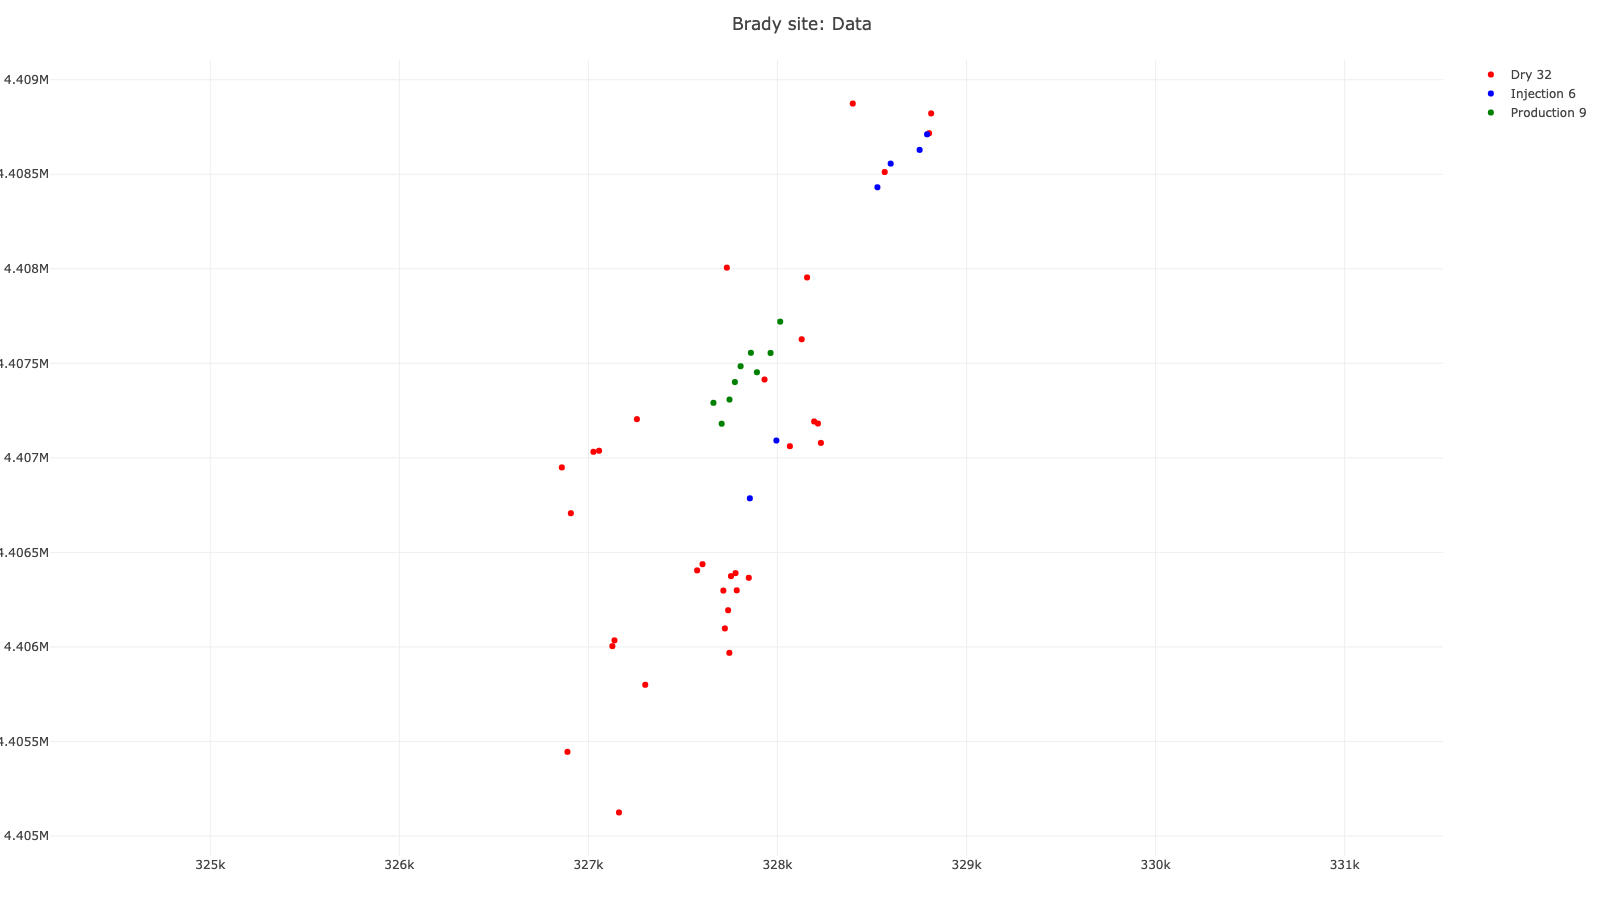
\includegraphics{../map/dataset-set01-v9-inv.png}
\caption{dataset-set01-v9-inv}
\end{figure}

    \hypertarget{perform-ml-analyses}{%
\subsection{Perform ML analyses}\label{perform-ml-analyses}}

For the ML analyses, the data tensor can be flattened into a data matrix
by using two different approaches:

\begin{itemize}
\tightlist
\item
  Type 1: Merge depth and attribute tensor dimensions; in this way, the
  focus of the ML analysis is on finding the features associated with
  the well locations
\item
  Type 2: Merge depth and location tensor dimensions; in this way, the
  focus of the ML analysis is on finding the features associated with
  the well attributes
\end{itemize}

After that the \textbf{NMFk} algorithm will factorize the data matrix
\texttt{X} into \texttt{W} and \texttt{H} matrices. For more
information, check out the
\href{https://github.com/SmartTensors/NMFk.jl}{\textbf{NMFk} website}

    \hypertarget{type-1-flattening-focus-on-well-locations}{%
\subsubsection{Type 1 flattening: Focus on well
locations}\label{type-1-flattening-focus-on-well-locations}}

\hypertarget{flatten-the-tensor-into-a-matrix}{%
\paragraph{Flatten the tensor into a
matrix}\label{flatten-the-tensor-into-a-matrix}}

    \begin{tcolorbox}[breakable, size=fbox, boxrule=1pt, pad at break*=1mm,colback=cellbackground, colframe=cellborder]
\prompt{In}{incolor}{18}{\boxspacing}
\begin{Verbatim}[commandchars=\\\{\}]
\PY{n}{Xdaln} \PY{o}{=} \PY{n}{reshape}\PY{p}{(}\PY{n}{Tn}\PY{p}{,} \PY{p}{(}\PY{n}{depth} \PY{o}{*} \PY{n}{length}\PY{p}{(}\PY{n}{attributes\PYZus{}process}\PY{p}{)}\PY{p}{)}\PY{p}{,} \PY{n}{length}\PY{p}{(}\PY{n}{locations}\PY{p}{)}\PY{p}{)}\PY{p}{;}
\end{Verbatim}
\end{tcolorbox}

    Matrix rows merge the depth and attribute dimensions.

Matrix columns represent the well locations.

    \hypertarget{perform-nmfk-analyses}{%
\paragraph{Perform NMFk analyses}\label{perform-nmfk-analyses}}

    \begin{tcolorbox}[breakable, size=fbox, boxrule=1pt, pad at break*=1mm,colback=cellbackground, colframe=cellborder]
\prompt{In}{incolor}{19}{\boxspacing}
\begin{Verbatim}[commandchars=\\\{\}]
\PY{n}{W}\PY{p}{,} \PY{n}{H}\PY{p}{,} \PY{n}{fitquality}\PY{p}{,} \PY{n}{robustness}\PY{p}{,} \PY{n}{aic} \PY{o}{=} \PY{n}{NMFk}\PY{o}{.}\PY{n}{execute}\PY{p}{(}\PY{n}{Xdaln}\PY{p}{,} \PY{n}{nkrange}\PY{p}{,} \PY{n}{nruns}\PY{p}{;} \PY{n}{resultdir}\PY{o}{=}\PY{n}{resultdir}\PY{p}{,} \PY{n}{casefilename}\PY{o}{=}\PY{l+s}{\PYZdq{}}\PY{l+s}{n}\PY{l+s}{m}\PY{l+s}{f}\PY{l+s}{k}\PY{l+s}{\PYZhy{}}\PY{l+s}{d}\PY{l+s}{a}\PY{l+s}{l}\PY{l+s}{n}\PY{l+s}{\PYZhy{}}\PY{l+s+si}{\PYZdl{}}\PY{p}{(}\PY{n}{join}\PY{p}{(}\PY{n}{size}\PY{p}{(}\PY{n}{Xdaln}\PY{p}{)}\PY{p}{,} \PY{l+s+sc}{\PYZsq{}\PYZus{}\PYZsq{}}\PY{p}{)}\PY{p}{)}\PY{l+s}{\PYZdq{}}\PY{p}{,} \PY{n}{load}\PY{o}{=}\PY{k+kc}{true}\PY{p}{)}
\PY{n}{W}\PY{p}{,} \PY{n}{H}\PY{p}{,} \PY{n}{fitquality}\PY{p}{,} \PY{n}{robustness}\PY{p}{,} \PY{n}{aic} \PY{o}{=} \PY{n}{NMFk}\PY{o}{.}\PY{n}{load}\PY{p}{(}\PY{n}{nkrange}\PY{p}{,} \PY{n}{nruns}\PY{p}{;} \PY{n}{resultdir}\PY{o}{=}\PY{n}{resultdir}\PY{p}{,} \PY{n}{casefilename}\PY{o}{=}\PY{l+s}{\PYZdq{}}\PY{l+s}{n}\PY{l+s}{m}\PY{l+s}{f}\PY{l+s}{k}\PY{l+s}{\PYZhy{}}\PY{l+s}{d}\PY{l+s}{a}\PY{l+s}{l}\PY{l+s}{n}\PY{l+s}{\PYZhy{}}\PY{l+s+si}{\PYZdl{}}\PY{p}{(}\PY{n}{join}\PY{p}{(}\PY{n}{size}\PY{p}{(}\PY{n}{Xdaln}\PY{p}{)}\PY{p}{,} \PY{l+s+sc}{\PYZsq{}\PYZus{}\PYZsq{}}\PY{p}{)}\PY{p}{)}\PY{l+s}{\PYZdq{}}\PY{p}{)}\PY{p}{;}
\end{Verbatim}
\end{tcolorbox}

    \begin{Verbatim}[commandchars=\\\{\}]
Signals:  2 Fit:     17906.11 Silhouette:    0.6571116 AIC:    -944054.7
Signals:  3 Fit:     15067.48 Silhouette:    0.2121185 AIC:    -981003.7
Signals:  4 Fit:     12811.86 Silhouette:  -0.03854946 AIC:     -1014443
Signals:  5 Fit:     10966.81 Silhouette:    0.4108927 AIC:     -1045640
Signals:  6 Fit:     9570.522 Silhouette:    0.4704617 AIC:     -1070343
Signals:  7 Fit:     8398.009 Silhouette:   -0.2070509 AIC:     -1093198
Signals:  8 Fit:     7428.398 Silhouette:   -0.2601539 AIC:     -1113361
Signals:  2 Fit:     17906.11 Silhouette:    0.6571116 AIC:    -944054.7
Signals:  3 Fit:     15067.48 Silhouette:    0.2121185 AIC:    -981003.7
Signals:  4 Fit:     12811.86 Silhouette:  -0.03854946 AIC:     -1014443
Signals:  5 Fit:     10966.81 Silhouette:    0.4108927 AIC:     -1045640
Signals:  6 Fit:     9570.522 Silhouette:    0.4704617 AIC:     -1070343
Signals:  7 Fit:     8398.009 Silhouette:   -0.2070509 AIC:     -1093198
Signals:  8 Fit:     7428.398 Silhouette:   -0.2601539 AIC:     -1113361
    \end{Verbatim}

    \begin{Verbatim}[commandchars=\\\{\}]
┌ Info: Results
└ @ NMFk /Users/vvv/.julia/dev/NMFk/src/NMFkExecute.jl:15
┌ Info: Optimal solution: 6 signals
└ @ NMFk /Users/vvv/.julia/dev/NMFk/src/NMFkExecute.jl:20
    \end{Verbatim}

    \begin{Verbatim}[commandchars=\\\{\}]
Signals:  2 Fit:     17906.11 Silhouette:    0.6571116 AIC:    -944054.7
Signals:  3 Fit:     15067.48 Silhouette:    0.2121185 AIC:    -981003.7
Signals:  4 Fit:     12811.86 Silhouette:  -0.03854946 AIC:     -1014443
Signals:  5 Fit:     10966.81 Silhouette:    0.4108927 AIC:     -1045640
Signals:  6 Fit:     9570.522 Silhouette:    0.4704617 AIC:     -1070343
Signals:  7 Fit:     8398.009 Silhouette:   -0.2070509 AIC:     -1093198
Signals:  8 Fit:     7428.398 Silhouette:   -0.2601539 AIC:     -1113361
    \end{Verbatim}

    \begin{Verbatim}[commandchars=\\\{\}]
┌ Info: Optimal solution: 6 signals
└ @ NMFk /Users/vvv/.julia/dev/NMFk/src/NMFkIO.jl:30
    \end{Verbatim}

    Here, the \textbf{NMFk} results are loaded from a prior ML run.

As seen from the output above, the \textbf{NMFk} analyses identified
that the optimal number of geothermal signatures in the dataset
\textbf{6}.

Solutions with a number of signatures less than \textbf{6} are
underfitting.

Solutions with a number of signatures greater than \textbf{6} are
overfitting and unacceptable.

The set of acceptable solutions are defined by the \textbf{NMFk}
algorithm as follows:

    \begin{tcolorbox}[breakable, size=fbox, boxrule=1pt, pad at break*=1mm,colback=cellbackground, colframe=cellborder]
\prompt{In}{incolor}{20}{\boxspacing}
\begin{Verbatim}[commandchars=\\\{\}]
\PY{n}{NMFk}\PY{o}{.}\PY{n}{getks}\PY{p}{(}\PY{n}{nkrange}\PY{p}{,} \PY{n}{robustness}\PY{p}{[}\PY{n}{nkrange}\PY{p}{]}\PY{p}{)}
\end{Verbatim}
\end{tcolorbox}

            \begin{tcolorbox}[breakable, size=fbox, boxrule=.5pt, pad at break*=1mm, opacityfill=0]
\prompt{Out}{outcolor}{20}{\boxspacing}
\begin{Verbatim}[commandchars=\\\{\}]
3-element Array\{Int64,1\}:
 2
 5
 6
\end{Verbatim}
\end{tcolorbox}
        
    The acceptable solutions contain 2, 5 and 6 signatures.

    \hypertarget{post-process-nmfk-results}{%
\paragraph{Post-process NMFk results}\label{post-process-nmfk-results}}

\hypertarget{number-of-signatures}{%
\paragraph{Number of signatures}\label{number-of-signatures}}

Below is a plot representing solution quality (fit) and silhouette width
(robustness) for different numbers of signatures \texttt{k}:

    \begin{tcolorbox}[breakable, size=fbox, boxrule=1pt, pad at break*=1mm,colback=cellbackground, colframe=cellborder]
\prompt{In}{incolor}{21}{\boxspacing}
\begin{Verbatim}[commandchars=\\\{\}]
\PY{n}{NMFk}\PY{o}{.}\PY{n}{plot\PYZus{}signal\PYZus{}selecton}\PY{p}{(}\PY{n}{nkrange}\PY{p}{,} \PY{n}{fitquality}\PY{p}{,} \PY{n}{robustness}\PY{p}{;} \PY{n}{figuredir}\PY{o}{=}\PY{l+s}{\PYZdq{}}\PY{l+s+si}{\PYZdl{}figuredir}\PY{l+s}{\PYZhy{}}\PY{l+s+si}{\PYZdl{}}\PY{p}{(}\PY{n}{nruns}\PY{p}{)}\PY{l+s}{\PYZhy{}}\PY{l+s}{d}\PY{l+s}{a}\PY{l+s}{l}\PY{l+s}{n}\PY{l+s}{\PYZdq{}}\PY{p}{,} \PY{n}{xtitle}\PY{o}{=}\PY{l+s}{\PYZdq{}}\PY{l+s}{N}\PY{l+s}{u}\PY{l+s}{m}\PY{l+s}{b}\PY{l+s}{e}\PY{l+s}{r}\PY{l+s}{ }\PY{l+s}{o}\PY{l+s}{f}\PY{l+s}{ }\PY{l+s}{s}\PY{l+s}{i}\PY{l+s}{g}\PY{l+s}{n}\PY{l+s}{a}\PY{l+s}{t}\PY{l+s}{u}\PY{l+s}{r}\PY{l+s}{e}\PY{l+s}{s}\PY{l+s}{\PYZdq{}}\PY{p}{)}
\end{Verbatim}
\end{tcolorbox}

    \begin{center}
    \adjustimage{max size={0.9\linewidth}{0.9\paperheight}}{Brady_files/Brady_48_0.png}
    \end{center}
    { \hspace*{\fill} \\}
    
    \begin{Verbatim}[commandchars=\\\{\}]

    \end{Verbatim}

    The plot above also demonstrates that the acceptable solutions contain
2, 5 and 6 signatures.

\hypertarget{analysis-of-all-the-acceptable-solutions}{%
\paragraph{Analysis of all the acceptable
solutions}\label{analysis-of-all-the-acceptable-solutions}}

The ML solutions containing an acceptable number of signatures are
further analyzed as follows:

    \begin{tcolorbox}[breakable, size=fbox, boxrule=1pt, pad at break*=1mm,colback=cellbackground, colframe=cellborder]
\prompt{In}{incolor}{22}{\boxspacing}
\begin{Verbatim}[commandchars=\\\{\}]
\PY{n}{NMFk}\PY{o}{.}\PY{n}{clusterresults}\PY{p}{(}\PY{n}{NMFk}\PY{o}{.}\PY{n}{getks}\PY{p}{(}\PY{n}{nkrange}\PY{p}{,} \PY{n}{robustness}\PY{p}{[}\PY{n}{nkrange}\PY{p}{]}\PY{p}{)}\PY{p}{,} \PY{n}{W}\PY{p}{,} \PY{n}{H}\PY{p}{,} \PY{n}{attributes\PYZus{}process\PYZus{}long}\PY{p}{,} \PY{n}{locations}\PY{p}{;} \PY{n}{loadassignements}\PY{o}{=}\PY{k+kc}{true}\PY{p}{,} \PY{n}{lon}\PY{o}{=}\PY{n}{xcoord}\PY{p}{,} \PY{n}{lat}\PY{o}{=}\PY{n}{ycoord}\PY{p}{,} \PY{n}{Wsize}\PY{o}{=}\PY{n}{depth}\PY{p}{,} \PY{n}{Wcasefilename}\PY{o}{=}\PY{l+s}{\PYZdq{}}\PY{l+s}{a}\PY{l+s}{t}\PY{l+s}{t}\PY{l+s}{r}\PY{l+s}{i}\PY{l+s}{b}\PY{l+s}{u}\PY{l+s}{t}\PY{l+s}{e}\PY{l+s}{s}\PY{l+s}{\PYZdq{}}\PY{p}{,} \PY{n}{Hcasefilename}\PY{o}{=}\PY{l+s}{\PYZdq{}}\PY{l+s}{l}\PY{l+s}{o}\PY{l+s}{c}\PY{l+s}{a}\PY{l+s}{t}\PY{l+s}{i}\PY{l+s}{o}\PY{l+s}{n}\PY{l+s}{s}\PY{l+s}{\PYZdq{}}\PY{p}{,} \PY{n}{resultdir}\PY{o}{=}\PY{n}{resultdir} \PY{o}{*} \PY{l+s}{\PYZdq{}}\PY{l+s}{\PYZhy{}}\PY{l+s+si}{\PYZdl{}}\PY{p}{(}\PY{n}{nruns}\PY{p}{)}\PY{l+s}{\PYZhy{}}\PY{l+s}{d}\PY{l+s}{a}\PY{l+s}{l}\PY{l+s}{n}\PY{l+s}{\PYZdq{}}\PY{p}{,} \PY{n}{figuredir}\PY{o}{=}\PY{n}{figuredir} \PY{o}{*} \PY{l+s}{\PYZdq{}}\PY{l+s}{\PYZhy{}}\PY{l+s+si}{\PYZdl{}}\PY{p}{(}\PY{n}{nruns}\PY{p}{)}\PY{l+s}{\PYZhy{}}\PY{l+s}{d}\PY{l+s}{a}\PY{l+s}{l}\PY{l+s}{n}\PY{l+s}{\PYZdq{}}\PY{p}{,} \PY{n}{hover}\PY{o}{=}\PY{l+s}{\PYZdq{}}\PY{l+s}{W}\PY{l+s}{e}\PY{l+s}{l}\PY{l+s}{l}\PY{l+s}{:}\PY{l+s}{ }\PY{l+s}{\PYZdq{}} \PY{o}{.*} \PY{n}{locations} \PY{o}{.*} \PY{l+s}{\PYZdq{}}\PY{l+s}{\PYZlt{}}\PY{l+s}{b}\PY{l+s}{r}\PY{l+s}{\PYZgt{}}\PY{l+s}{\PYZdq{}} \PY{o}{.*} \PY{l+s}{\PYZdq{}}\PY{l+s}{W}\PY{l+s}{e}\PY{l+s}{l}\PY{l+s}{l}\PY{l+s}{T}\PY{l+s}{y}\PY{l+s}{p}\PY{l+s}{e}\PY{l+s}{:}\PY{l+s}{ }\PY{l+s}{\PYZdq{}} \PY{o}{.*} \PY{n}{String}\PY{o}{.}\PY{p}{(}\PY{n}{welltype}\PY{p}{)} \PY{o}{.*} \PY{l+s}{\PYZdq{}}\PY{l+s}{\PYZlt{}}\PY{l+s}{b}\PY{l+s}{r}\PY{l+s}{\PYZgt{}}\PY{l+s}{\PYZdq{}} \PY{o}{.*} \PY{n}{production}\PY{p}{,} \PY{n}{Wmatrix\PYZus{}font\PYZus{}size}\PY{o}{=}\PY{l+m+mi}{4}\PY{n}{Gadfly}\PY{o}{.}\PY{n}{pt}\PY{p}{,} \PY{n}{biplotcolor}\PY{o}{=}\PY{o}{:}\PY{n}{WH}\PY{p}{,} \PY{n}{biplotlabel}\PY{o}{=}\PY{o}{:}\PY{n}{WH}\PY{p}{)}
\end{Verbatim}
\end{tcolorbox}

    \begin{Verbatim}[commandchars=\\\{\}]
┌ Info: Number of signals: 2
└ @ NMFk /Users/vvv/.julia/dev/NMFk/src/NMFkPostprocess.jl:144
    \end{Verbatim}

    \begin{Verbatim}[commandchars=\\\{\}]
Signal importance (high->low): [2, 1]
    \end{Verbatim}

    \begin{Verbatim}[commandchars=\\\{\}]
┌ Info: Locations (signals=2)
└ @ NMFk /Users/vvv/.julia/dev/NMFk/src/NMFkPostprocess.jl:148
┌ Warning: type
Clustering.KmeansResult\{Core.Array\{Core.Float64,2\},Core.Float64,Core.Int64\} not
present in workspace; reconstructing
└ @ JLD /Users/vvv/.julia/packages/JLD/nQ9iW/src/jld\_types.jl:697
┌ Info: Robust k-means analysis results are loaded from file results-
set00-v9-inv-750-1000-daln/Hmatrix-2-2\_47-1000.jld!
└ @ NMFk /Users/vvv/.julia/dev/NMFk/src/NMFkCluster.jl:67
┌ Warning: Procedure to find unique signals could not identify a solution {\ldots}
└ @ NMFk /Users/vvv/.julia/dev/NMFk/src/NMFkCluster.jl:158
┌ Warning: Procedure to find unique signals could not identify a solution {\ldots}
└ @ NMFk /Users/vvv/.julia/dev/NMFk/src/NMFkCluster.jl:158
┌ Warning: type
Clustering.KmeansResult\{Core.Array\{Core.Float64,2\},Core.Float64,Core.Int64\} not
present in workspace; reconstructing
└ @ JLD /Users/vvv/.julia/packages/JLD/nQ9iW/src/jld\_types.jl:697
┌ Info: Robust k-means analysis results are loaded from file results-
set00-v9-inv-750-1000-daln/Wmatrix-2-2\_14-1000.jld!
└ @ NMFk /Users/vvv/.julia/dev/NMFk/src/NMFkCluster.jl:67
┌ Warning: Procedure to find unique signals could not identify a solution {\ldots}
└ @ NMFk /Users/vvv/.julia/dev/NMFk/src/NMFkCluster.jl:158
┌ Warning: Procedure to find unique signals could not identify a solution {\ldots}
└ @ NMFk /Users/vvv/.julia/dev/NMFk/src/NMFkCluster.jl:158
┌ Info: Signal A -> A Count: 24
└ @ NMFk /Users/vvv/.julia/dev/NMFk/src/NMFkPostprocess.jl:255
    \end{Verbatim}

    
    \begin{Verbatim}[commandchars=\\\{\}]
24×2 Array\{Any,2\}:
 "MGI-2"       1.0
 "B7"          0.971874
 "MG-2(SP-2)"  0.957147
 "64-1"        0.906381
 "B4"          0.902571
 "B6"          0.897107
 "B5"          0.874384
 "MG-1(SP-1)"  0.828417
 "B3"          0.82034
 "68A-1"       0.80013
 "B5A"         0.78864
 "MGI-1"       0.732217
 "68B-1"       0.696522
 "77-1"        0.655878
 "17-31"       0.57376
 "B8"          0.528089
 "55-1"        0.491206
 "EE-1"        0.487324
 "56-1"        0.455524
 "57-1"        0.43842
 "56B-1"       0.413443
 "18-1"        0.395716
 "18A-1"       0.370733
 "22-13"       0.269227
    \end{Verbatim}

    
    \begin{Verbatim}[commandchars=\\\{\}]
┌ Info: Signal B -> B Count: 23
└ @ NMFk /Users/vvv/.julia/dev/NMFk/src/NMFkPostprocess.jl:255
┌ Info: Signal A (S1) (k-means clustering)
└ @ NMFk /Users/vvv/.julia/dev/NMFk/src/NMFkPostprocess.jl:272
    \end{Verbatim}

    
    \begin{Verbatim}[commandchars=\\\{\}]
23×2 Array\{Any,2\}:
 "18-31"   1.0
 "18B-31"  0.960836
 "56A-1"   0.878124
 "81-1"    0.859001
 "48A-1"   0.849051
 "81A-1"   0.838298
 "47C-1"   0.826181
 "B2"      0.804453
 "81B-1"   0.796872
 "46-1"    0.765556
 "46A-1"   0.763833
 "BCH-3"   0.735382
 "18D-31"  0.726398
 "15-12"   0.719203
 "27-1"    0.66714
 "81-11"   0.659873
 "88-11"   0.641011
 "BCH-1"   0.61491
 "B1"      0.58518
 "47A-1"   0.533141
 "BCH-2"   0.494268
 "26-12"   0.482354
 "82A-11"  0.354477
    \end{Verbatim}

    
    \begin{center}
    \adjustimage{max size={0.9\linewidth}{0.9\paperheight}}{Brady_files/Brady_50_6.png}
    \end{center}
    { \hspace*{\fill} \\}
    
    \begin{Verbatim}[commandchars=\\\{\}]
┌ Info: Signal B (S2) (k-means clustering)
└ @ NMFk /Users/vvv/.julia/dev/NMFk/src/NMFkPostprocess.jl:272
    \end{Verbatim}

    \begin{center}
    \adjustimage{max size={0.9\linewidth}{0.9\paperheight}}{Brady_files/Brady_50_8.png}
    \end{center}
    { \hspace*{\fill} \\}
    
    \begin{Verbatim}[commandchars=\\\{\}]

    \end{Verbatim}

    \begin{center}
    \adjustimage{max size={0.9\linewidth}{0.9\paperheight}}{Brady_files/Brady_50_10.png}
    \end{center}
    { \hspace*{\fill} \\}
    
    \begin{center}
    \adjustimage{max size={0.9\linewidth}{0.9\paperheight}}{Brady_files/Brady_50_11.png}
    \end{center}
    { \hspace*{\fill} \\}
    
    \begin{Verbatim}[commandchars=\\\{\}]

    \end{Verbatim}

    \begin{center}
    \adjustimage{max size={0.9\linewidth}{0.9\paperheight}}{Brady_files/Brady_50_13.png}
    \end{center}
    { \hspace*{\fill} \\}
    
    \begin{Verbatim}[commandchars=\\\{\}]

    \end{Verbatim}

    
    \begin{Verbatim}[commandchars=\\\{\}]
1×2 Array\{Any,2\}:
 "Inverse distance from contacts"  0.619519
    \end{Verbatim}

    
    
    \begin{Verbatim}[commandchars=\\\{\}]
13×2 Array\{Any,2\}:
 "Unit thickness"                1.0
 "Inverse distance from faults"  0.957468
 "Fault density"                 0.761708
 "Coulomb shear stress"          0.74607
 "Normal stress"                 0.737061
 "Faulting"                      0.706576
 "Fault intersection density"    0.702918
 "Dilation"                      0.635119
 "Fault dilation tendency"       0.605243
 "Fault curvature"               0.538705
 "Lithology"                     0.488473
 "Fault slip tendency"           0.41415
 "Temperature"                   0.131901
    \end{Verbatim}

    
    \begin{center}
    \adjustimage{max size={0.9\linewidth}{0.9\paperheight}}{Brady_files/Brady_50_17.png}
    \end{center}
    { \hspace*{\fill} \\}
    
    \begin{Verbatim}[commandchars=\\\{\}]
┌ Info: Attributes (signals=2)
└ @ NMFk /Users/vvv/.julia/dev/NMFk/src/NMFkPostprocess.jl:322
┌ Info: Signal A (S2) Count: 13
└ @ NMFk /Users/vvv/.julia/dev/NMFk/src/NMFkPostprocess.jl:335
┌ Info: Signal B (S1) Count: 1
└ @ NMFk /Users/vvv/.julia/dev/NMFk/src/NMFkPostprocess.jl:335
┌ Info: Signal B -> A Count: 1
└ @ NMFk /Users/vvv/.julia/dev/NMFk/src/NMFkPostprocess.jl:345
┌ Info: Signal A -> B Count: 13
└ @ NMFk /Users/vvv/.julia/dev/NMFk/src/NMFkPostprocess.jl:345
┌ Info: Signal A (remapped k-means clustering)
└ @ NMFk /Users/vvv/.julia/dev/NMFk/src/NMFkPostprocess.jl:360
┌ Info: Signal B (remapped k-means clustering)
└ @ NMFk /Users/vvv/.julia/dev/NMFk/src/NMFkPostprocess.jl:360
    \end{Verbatim}

    \begin{center}
    \adjustimage{max size={0.9\linewidth}{0.9\paperheight}}{Brady_files/Brady_50_19.png}
    \end{center}
    { \hspace*{\fill} \\}
    
    \begin{Verbatim}[commandchars=\\\{\}]

    \end{Verbatim}

    \begin{center}
    \adjustimage{max size={0.9\linewidth}{0.9\paperheight}}{Brady_files/Brady_50_21.png}
    \end{center}
    { \hspace*{\fill} \\}
    
    \begin{center}
    \adjustimage{max size={0.9\linewidth}{0.9\paperheight}}{Brady_files/Brady_50_22.png}
    \end{center}
    { \hspace*{\fill} \\}
    
    \begin{Verbatim}[commandchars=\\\{\}]

    \end{Verbatim}

    \begin{center}
    \adjustimage{max size={0.9\linewidth}{0.9\paperheight}}{Brady_files/Brady_50_24.png}
    \end{center}
    { \hspace*{\fill} \\}
    
    \begin{center}
    \adjustimage{max size={0.9\linewidth}{0.9\paperheight}}{Brady_files/Brady_50_25.png}
    \end{center}
    { \hspace*{\fill} \\}
    
    \begin{Verbatim}[commandchars=\\\{\}]

    \end{Verbatim}

    \begin{center}
    \adjustimage{max size={0.9\linewidth}{0.9\paperheight}}{Brady_files/Brady_50_27.png}
    \end{center}
    { \hspace*{\fill} \\}
    
    \begin{Verbatim}[commandchars=\\\{\}]
Signal importance (high->low): [1, 3, 5, 4, 2]
    \end{Verbatim}

    \begin{Verbatim}[commandchars=\\\{\}]
┌ Info: Number of signals: 5
└ @ NMFk /Users/vvv/.julia/dev/NMFk/src/NMFkPostprocess.jl:144
┌ Info: Locations (signals=5)
└ @ NMFk /Users/vvv/.julia/dev/NMFk/src/NMFkPostprocess.jl:148
┌ Warning: type
Clustering.KmeansResult\{Core.Array\{Core.Float64,2\},Core.Float64,Core.Int64\} not
present in workspace; reconstructing
└ @ JLD /Users/vvv/.julia/packages/JLD/nQ9iW/src/jld\_types.jl:697
┌ Info: Robust k-means analysis results are loaded from file results-
set00-v9-inv-750-1000-daln/Hmatrix-5-5\_47-1000.jld!
└ @ NMFk /Users/vvv/.julia/dev/NMFk/src/NMFkCluster.jl:67
┌ Warning: Procedure to find unique signals could not identify a solution {\ldots}
└ @ NMFk /Users/vvv/.julia/dev/NMFk/src/NMFkCluster.jl:158
┌ Warning: Procedure to find unique signals could not identify a solution {\ldots}
└ @ NMFk /Users/vvv/.julia/dev/NMFk/src/NMFkCluster.jl:158
┌ Warning: Procedure to find unique signals could not identify a solution {\ldots}
└ @ NMFk /Users/vvv/.julia/dev/NMFk/src/NMFkCluster.jl:158
┌ Warning: Procedure to find unique signals could not identify a solution {\ldots}
└ @ NMFk /Users/vvv/.julia/dev/NMFk/src/NMFkCluster.jl:158
┌ Warning: Procedure to find unique signals could not identify a solution {\ldots}
└ @ NMFk /Users/vvv/.julia/dev/NMFk/src/NMFkCluster.jl:158
┌ Warning: type
Clustering.KmeansResult\{Core.Array\{Core.Float64,2\},Core.Float64,Core.Int64\} not
present in workspace; reconstructing
└ @ JLD /Users/vvv/.julia/packages/JLD/nQ9iW/src/jld\_types.jl:697
┌ Info: Robust k-means analysis results are loaded from file results-
set00-v9-inv-750-1000-daln/Wmatrix-5-5\_14-1000.jld!
└ @ NMFk /Users/vvv/.julia/dev/NMFk/src/NMFkCluster.jl:67
    \end{Verbatim}

    
    \begin{Verbatim}[commandchars=\\\{\}]
11×2 Array\{Any,2\}:
 "MG-2(SP-2)"  1.0
 "56-1"        0.833071
 "18-31"       0.803582
 "18B-31"      0.79762
 "64-1"        0.771609
 "57-1"        0.731212
 "17-31"       0.675958
 "81B-1"       0.638129
 "18D-31"      0.542359
 "55-1"        0.482608
 "22-13"       0.384279
    \end{Verbatim}

    
    
    \begin{Verbatim}[commandchars=\\\{\}]
11×2 Array\{Any,2\}:
 "68A-1"       1.0
 "MG-1(SP-1)"  0.760228
 "B7"          0.583165
 "B3"          0.579901
 "B4"          0.559561
 "MGI-2"       0.550751
 "68B-1"       0.549639
 "B6"          0.533677
 "77-1"        0.51494
 "B5A"         0.492662
 "B5"          0.444441
    \end{Verbatim}

    
    
    \begin{Verbatim}[commandchars=\\\{\}]
9×2 Array\{Any,2\}:
 "56B-1"  1.0
 "B2"     0.952516
 "EE-1"   0.837563
 "48A-1"  0.787595
 "B8"     0.779397
 "B1"     0.711321
 "47C-1"  0.625562
 "81-11"  0.574423
 "47A-1"  0.549964
    \end{Verbatim}

    
    
    \begin{Verbatim}[commandchars=\\\{\}]
8×2 Array\{Any,2\}:
 "18-1"    1.0
 "82A-11"  0.947022
 "18A-1"   0.723864
 "88-11"   0.57605
 "15-12"   0.515703
 "BCH-3"   0.472471
 "27-1"    0.439353
 "56A-1"   0.3504
    \end{Verbatim}

    
    
    \begin{Verbatim}[commandchars=\\\{\}]
8×2 Array\{Any,2\}:
 "26-12"  0.82344
 "BCH-2"  0.822391
 "BCH-1"  0.766974
 "46A-1"  0.586862
 "81-1"   0.570404
 "81A-1"  0.545145
 "46-1"   0.529248
 "MGI-1"  0.456212
    \end{Verbatim}

    
    \begin{center}
    \adjustimage{max size={0.9\linewidth}{0.9\paperheight}}{Brady_files/Brady_50_35.png}
    \end{center}
    { \hspace*{\fill} \\}
    
    \begin{Verbatim}[commandchars=\\\{\}]
┌ Warning: Procedure to find unique signals could not identify a solution {\ldots}
└ @ NMFk /Users/vvv/.julia/dev/NMFk/src/NMFkCluster.jl:158
┌ Warning: Procedure to find unique signals could not identify a solution {\ldots}
└ @ NMFk /Users/vvv/.julia/dev/NMFk/src/NMFkCluster.jl:158
┌ Warning: Procedure to find unique signals could not identify a solution {\ldots}
└ @ NMFk /Users/vvv/.julia/dev/NMFk/src/NMFkCluster.jl:158
┌ Info: Signal A -> A Count: 11
└ @ NMFk /Users/vvv/.julia/dev/NMFk/src/NMFkPostprocess.jl:255
┌ Info: Signal B -> B Count: 11
└ @ NMFk /Users/vvv/.julia/dev/NMFk/src/NMFkPostprocess.jl:255
┌ Info: Signal C -> C Count: 9
└ @ NMFk /Users/vvv/.julia/dev/NMFk/src/NMFkPostprocess.jl:255
┌ Info: Signal D -> D Count: 8
└ @ NMFk /Users/vvv/.julia/dev/NMFk/src/NMFkPostprocess.jl:255
┌ Info: Signal E -> E Count: 8
└ @ NMFk /Users/vvv/.julia/dev/NMFk/src/NMFkPostprocess.jl:255
┌ Info: Signal A (S3) (k-means clustering)
└ @ NMFk /Users/vvv/.julia/dev/NMFk/src/NMFkPostprocess.jl:272
┌ Info: Signal B (S2) (k-means clustering)
└ @ NMFk /Users/vvv/.julia/dev/NMFk/src/NMFkPostprocess.jl:272
┌ Info: Signal C (S1) (k-means clustering)
└ @ NMFk /Users/vvv/.julia/dev/NMFk/src/NMFkPostprocess.jl:272
┌ Info: Signal D (S4) (k-means clustering)
└ @ NMFk /Users/vvv/.julia/dev/NMFk/src/NMFkPostprocess.jl:272
┌ Info: Signal E (S5) (k-means clustering)
└ @ NMFk /Users/vvv/.julia/dev/NMFk/src/NMFkPostprocess.jl:272
    \end{Verbatim}

    \begin{center}
    \adjustimage{max size={0.9\linewidth}{0.9\paperheight}}{Brady_files/Brady_50_37.png}
    \end{center}
    { \hspace*{\fill} \\}
    
    \begin{Verbatim}[commandchars=\\\{\}]

    \end{Verbatim}

    \begin{center}
    \adjustimage{max size={0.9\linewidth}{0.9\paperheight}}{Brady_files/Brady_50_39.png}
    \end{center}
    { \hspace*{\fill} \\}
    
    \begin{center}
    \adjustimage{max size={0.9\linewidth}{0.9\paperheight}}{Brady_files/Brady_50_40.png}
    \end{center}
    { \hspace*{\fill} \\}
    
    \begin{Verbatim}[commandchars=\\\{\}]

    \end{Verbatim}

    \begin{center}
    \adjustimage{max size={0.9\linewidth}{0.9\paperheight}}{Brady_files/Brady_50_42.png}
    \end{center}
    { \hspace*{\fill} \\}
    
    \begin{Verbatim}[commandchars=\\\{\}]

    \end{Verbatim}

    
    \begin{Verbatim}[commandchars=\\\{\}]
7×2 Array\{Any,2\}:
 "Unit thickness"                0.849937
 "Inverse distance from faults"  0.680541
 "Fault intersection density"    0.629292
 "Fault dilation tendency"       0.501789
 "Fault curvature"               0.449738
 "Fault slip tendency"           0.365781
 "Temperature"                   0.123165
    \end{Verbatim}

    
    
    \begin{Verbatim}[commandchars=\\\{\}]
1×2 Array\{Any,2\}:
 "Inverse distance from contacts"  1.0
    \end{Verbatim}

    
    
    \begin{Verbatim}[commandchars=\\\{\}]
3×2 Array\{Any,2\}:
 "Faulting"       0.892846
 "Fault density"  0.880551
 "Dilation"       0.841464
    \end{Verbatim}

    
    
    \begin{Verbatim}[commandchars=\\\{\}]
1×2 Array\{Any,2\}:
 "Lithology"  0.89235
    \end{Verbatim}

    
    
    \begin{Verbatim}[commandchars=\\\{\}]
2×2 Array\{Any,2\}:
 "Coulomb shear stress"  0.826886
 "Normal stress"         0.820471
    \end{Verbatim}

    
    \begin{center}
    \adjustimage{max size={0.9\linewidth}{0.9\paperheight}}{Brady_files/Brady_50_49.png}
    \end{center}
    { \hspace*{\fill} \\}
    
    \begin{Verbatim}[commandchars=\\\{\}]
┌ Info: Attributes (signals=5)
└ @ NMFk /Users/vvv/.julia/dev/NMFk/src/NMFkPostprocess.jl:322
┌ Info: Signal A (S3) Count: 7
└ @ NMFk /Users/vvv/.julia/dev/NMFk/src/NMFkPostprocess.jl:335
┌ Info: Signal B (S1) Count: 3
└ @ NMFk /Users/vvv/.julia/dev/NMFk/src/NMFkPostprocess.jl:335
┌ Info: Signal C (S5) Count: 2
└ @ NMFk /Users/vvv/.julia/dev/NMFk/src/NMFkPostprocess.jl:335
┌ Info: Signal D (S2) Count: 1
└ @ NMFk /Users/vvv/.julia/dev/NMFk/src/NMFkPostprocess.jl:335
┌ Info: Signal E (S4) Count: 1
└ @ NMFk /Users/vvv/.julia/dev/NMFk/src/NMFkPostprocess.jl:335
┌ Info: Signal A -> A Count: 7
└ @ NMFk /Users/vvv/.julia/dev/NMFk/src/NMFkPostprocess.jl:345
┌ Info: Signal D -> B Count: 1
└ @ NMFk /Users/vvv/.julia/dev/NMFk/src/NMFkPostprocess.jl:345
┌ Info: Signal B -> C Count: 3
└ @ NMFk /Users/vvv/.julia/dev/NMFk/src/NMFkPostprocess.jl:345
┌ Info: Signal E -> D Count: 1
└ @ NMFk /Users/vvv/.julia/dev/NMFk/src/NMFkPostprocess.jl:345
┌ Info: Signal C -> E Count: 2
└ @ NMFk /Users/vvv/.julia/dev/NMFk/src/NMFkPostprocess.jl:345
┌ Info: Signal A (remapped k-means clustering)
└ @ NMFk /Users/vvv/.julia/dev/NMFk/src/NMFkPostprocess.jl:360
┌ Info: Signal B (remapped k-means clustering)
└ @ NMFk /Users/vvv/.julia/dev/NMFk/src/NMFkPostprocess.jl:360
┌ Info: Signal C (remapped k-means clustering)
└ @ NMFk /Users/vvv/.julia/dev/NMFk/src/NMFkPostprocess.jl:360
┌ Info: Signal D (remapped k-means clustering)
└ @ NMFk /Users/vvv/.julia/dev/NMFk/src/NMFkPostprocess.jl:360
┌ Info: Signal E (remapped k-means clustering)
└ @ NMFk /Users/vvv/.julia/dev/NMFk/src/NMFkPostprocess.jl:360
    \end{Verbatim}

    \begin{center}
    \adjustimage{max size={0.9\linewidth}{0.9\paperheight}}{Brady_files/Brady_50_51.png}
    \end{center}
    { \hspace*{\fill} \\}
    
    \begin{Verbatim}[commandchars=\\\{\}]

    \end{Verbatim}

    \begin{center}
    \adjustimage{max size={0.9\linewidth}{0.9\paperheight}}{Brady_files/Brady_50_53.png}
    \end{center}
    { \hspace*{\fill} \\}
    
    \begin{center}
    \adjustimage{max size={0.9\linewidth}{0.9\paperheight}}{Brady_files/Brady_50_54.png}
    \end{center}
    { \hspace*{\fill} \\}
    
    \begin{Verbatim}[commandchars=\\\{\}]

    \end{Verbatim}

    \begin{center}
    \adjustimage{max size={0.9\linewidth}{0.9\paperheight}}{Brady_files/Brady_50_56.png}
    \end{center}
    { \hspace*{\fill} \\}
    
    \begin{center}
    \adjustimage{max size={0.9\linewidth}{0.9\paperheight}}{Brady_files/Brady_50_57.png}
    \end{center}
    { \hspace*{\fill} \\}
    
    \begin{Verbatim}[commandchars=\\\{\}]

    \end{Verbatim}

    \begin{center}
    \adjustimage{max size={0.9\linewidth}{0.9\paperheight}}{Brady_files/Brady_50_59.png}
    \end{center}
    { \hspace*{\fill} \\}
    
    \begin{Verbatim}[commandchars=\\\{\}]
Signal importance (high->low): [1, 5, 2, 6, 4, 3]
    \end{Verbatim}

    \begin{Verbatim}[commandchars=\\\{\}]
┌ Info: Number of signals: 6
└ @ NMFk /Users/vvv/.julia/dev/NMFk/src/NMFkPostprocess.jl:144
┌ Info: Locations (signals=6)
└ @ NMFk /Users/vvv/.julia/dev/NMFk/src/NMFkPostprocess.jl:148
┌ Warning: type
Clustering.KmeansResult\{Core.Array\{Core.Float64,2\},Core.Float64,Core.Int64\} not
present in workspace; reconstructing
└ @ JLD /Users/vvv/.julia/packages/JLD/nQ9iW/src/jld\_types.jl:697
┌ Info: Robust k-means analysis results are loaded from file results-
set00-v9-inv-750-1000-daln/Hmatrix-6-6\_47-1000.jld!
└ @ NMFk /Users/vvv/.julia/dev/NMFk/src/NMFkCluster.jl:67
┌ Warning: Procedure to find unique signals could not identify a solution {\ldots}
└ @ NMFk /Users/vvv/.julia/dev/NMFk/src/NMFkCluster.jl:158
┌ Warning: Procedure to find unique signals could not identify a solution {\ldots}
└ @ NMFk /Users/vvv/.julia/dev/NMFk/src/NMFkCluster.jl:158
┌ Warning: Procedure to find unique signals could not identify a solution {\ldots}
└ @ NMFk /Users/vvv/.julia/dev/NMFk/src/NMFkCluster.jl:158
┌ Warning: Procedure to find unique signals could not identify a solution {\ldots}
└ @ NMFk /Users/vvv/.julia/dev/NMFk/src/NMFkCluster.jl:158
┌ Warning: Procedure to find unique signals could not identify a solution {\ldots}
└ @ NMFk /Users/vvv/.julia/dev/NMFk/src/NMFkCluster.jl:158
┌ Warning: Procedure to find unique signals could not identify a solution {\ldots}
└ @ NMFk /Users/vvv/.julia/dev/NMFk/src/NMFkCluster.jl:158
┌ Warning: type
Clustering.KmeansResult\{Core.Array\{Core.Float64,2\},Core.Float64,Core.Int64\} not
present in workspace; reconstructing
└ @ JLD /Users/vvv/.julia/packages/JLD/nQ9iW/src/jld\_types.jl:697
    \end{Verbatim}

    
    \begin{Verbatim}[commandchars=\\\{\}]
11×2 Array\{Any,2\}:
 "MG-1(SP-1)"  1.0
 "68B-1"       0.917059
 "77-1"        0.81018
 "B5A"         0.794163
 "68A-1"       0.771571
 "B5"          0.751175
 "B6"          0.726543
 "MGI-2"       0.712331
 "B7"          0.71064
 "B4"          0.671091
 "B3"          0.643308
    \end{Verbatim}

    
    
    \begin{Verbatim}[commandchars=\\\{\}]
10×2 Array\{Any,2\}:
 "82A-11"  1.0
 "88-11"   0.708797
 "18-1"    0.670833
 "27-1"    0.588465
 "18A-1"   0.586851
 "22-13"   0.530055
 "81B-1"   0.490522
 "18B-31"  0.450915
 "18D-31"  0.439487
 "18-31"   0.413683
    \end{Verbatim}

    
    
    \begin{Verbatim}[commandchars=\\\{\}]
7×2 Array\{Any,2\}:
 "MG-2(SP-2)"  1.0
 "64-1"        0.741999
 "MGI-1"       0.701663
 "56-1"        0.640372
 "57-1"        0.600702
 "17-31"       0.512659
 "55-1"        0.453248
    \end{Verbatim}

    
    
    \begin{Verbatim}[commandchars=\\\{\}]
7×2 Array\{Any,2\}:
 "B2"     1.0
 "EE-1"   0.68867
 "B8"     0.679526
 "56B-1"  0.56822
 "BCH-2"  0.521776
 "B1"     0.342468
 "81-11"  0.320946
    \end{Verbatim}

    
    
    \begin{Verbatim}[commandchars=\\\{\}]
6×2 Array\{Any,2\}:
 "BCH-3"  1.0
 "15-12"  0.904396
 "26-12"  0.808831
 "BCH-1"  0.795303
 "81-1"   0.7272
 "81A-1"  0.707665
    \end{Verbatim}

    
    
    \begin{Verbatim}[commandchars=\\\{\}]
6×2 Array\{Any,2\}:
 "47C-1"  1.0
 "46A-1"  0.943298
 "48A-1"  0.903309
 "46-1"   0.882457
 "47A-1"  0.751523
 "56A-1"  0.720315
    \end{Verbatim}

    
    \begin{center}
    \adjustimage{max size={0.9\linewidth}{0.9\paperheight}}{Brady_files/Brady_50_68.png}
    \end{center}
    { \hspace*{\fill} \\}
    
    \begin{Verbatim}[commandchars=\\\{\}]
┌ Info: Robust k-means analysis results are loaded from file results-
set00-v9-inv-750-1000-daln/Wmatrix-6-6\_14-1000.jld!
└ @ NMFk /Users/vvv/.julia/dev/NMFk/src/NMFkCluster.jl:67
┌ Warning: Procedure to find unique signals could not identify a solution {\ldots}
└ @ NMFk /Users/vvv/.julia/dev/NMFk/src/NMFkCluster.jl:158
┌ Info: Signal A -> A Count: 11
└ @ NMFk /Users/vvv/.julia/dev/NMFk/src/NMFkPostprocess.jl:255
┌ Info: Signal B -> B Count: 10
└ @ NMFk /Users/vvv/.julia/dev/NMFk/src/NMFkPostprocess.jl:255
┌ Info: Signal C -> C Count: 7
└ @ NMFk /Users/vvv/.julia/dev/NMFk/src/NMFkPostprocess.jl:255
┌ Info: Signal D -> D Count: 7
└ @ NMFk /Users/vvv/.julia/dev/NMFk/src/NMFkPostprocess.jl:255
┌ Info: Signal E -> E Count: 6
└ @ NMFk /Users/vvv/.julia/dev/NMFk/src/NMFkPostprocess.jl:255
┌ Info: Signal F -> F Count: 6
└ @ NMFk /Users/vvv/.julia/dev/NMFk/src/NMFkPostprocess.jl:255
┌ Info: Signal A (S3) (k-means clustering)
└ @ NMFk /Users/vvv/.julia/dev/NMFk/src/NMFkPostprocess.jl:272
┌ Info: Signal B (S4) (k-means clustering)
└ @ NMFk /Users/vvv/.julia/dev/NMFk/src/NMFkPostprocess.jl:272
┌ Info: Signal C (S6) (k-means clustering)
└ @ NMFk /Users/vvv/.julia/dev/NMFk/src/NMFkPostprocess.jl:272
┌ Info: Signal D (S2) (k-means clustering)
└ @ NMFk /Users/vvv/.julia/dev/NMFk/src/NMFkPostprocess.jl:272
┌ Info: Signal E (S5) (k-means clustering)
└ @ NMFk /Users/vvv/.julia/dev/NMFk/src/NMFkPostprocess.jl:272
┌ Info: Signal F (S1) (k-means clustering)
└ @ NMFk /Users/vvv/.julia/dev/NMFk/src/NMFkPostprocess.jl:272
    \end{Verbatim}

    \begin{center}
    \adjustimage{max size={0.9\linewidth}{0.9\paperheight}}{Brady_files/Brady_50_70.png}
    \end{center}
    { \hspace*{\fill} \\}
    
    \begin{Verbatim}[commandchars=\\\{\}]

    \end{Verbatim}

    \begin{center}
    \adjustimage{max size={0.9\linewidth}{0.9\paperheight}}{Brady_files/Brady_50_72.png}
    \end{center}
    { \hspace*{\fill} \\}
    
    \begin{center}
    \adjustimage{max size={0.9\linewidth}{0.9\paperheight}}{Brady_files/Brady_50_73.png}
    \end{center}
    { \hspace*{\fill} \\}
    
    \begin{Verbatim}[commandchars=\\\{\}]

    \end{Verbatim}

    \begin{center}
    \adjustimage{max size={0.9\linewidth}{0.9\paperheight}}{Brady_files/Brady_50_75.png}
    \end{center}
    { \hspace*{\fill} \\}
    
    \begin{Verbatim}[commandchars=\\\{\}]

    \end{Verbatim}

    
    \begin{Verbatim}[commandchars=\\\{\}]
1×2 Array\{Any,2\}:
 "Inverse distance from contacts"  1.0
    \end{Verbatim}

    
    
    \begin{Verbatim}[commandchars=\\\{\}]
1×2 Array\{Any,2\}:
 "Lithology"  0.864227
    \end{Verbatim}

    
    
    \begin{Verbatim}[commandchars=\\\{\}]
5×2 Array\{Any,2\}:
 "Fault intersection density"  0.534767
 "Fault dilation tendency"     0.494983
 "Fault curvature"             0.444422
 "Fault slip tendency"         0.367193
 "Temperature"                 0.136511
    \end{Verbatim}

    
    
    \begin{Verbatim}[commandchars=\\\{\}]
2×2 Array\{Any,2\}:
 "Unit thickness"                1.0
 "Inverse distance from faults"  0.778501
    \end{Verbatim}

    
    
    \begin{Verbatim}[commandchars=\\\{\}]
2×2 Array\{Any,2\}:
 "Normal stress"         0.896801
 "Coulomb shear stress"  0.845105
    \end{Verbatim}

    
    
    \begin{Verbatim}[commandchars=\\\{\}]
3×2 Array\{Any,2\}:
 "Fault density"  1.0
 "Faulting"       0.877916
 "Dilation"       0.834909
    \end{Verbatim}

    
    \begin{center}
    \adjustimage{max size={0.9\linewidth}{0.9\paperheight}}{Brady_files/Brady_50_83.png}
    \end{center}
    { \hspace*{\fill} \\}
    
    \begin{Verbatim}[commandchars=\\\{\}]
┌ Info: Attributes (signals=6)
└ @ NMFk /Users/vvv/.julia/dev/NMFk/src/NMFkPostprocess.jl:322
┌ Info: Signal A (S6) Count: 5
└ @ NMFk /Users/vvv/.julia/dev/NMFk/src/NMFkPostprocess.jl:335
┌ Info: Signal B (S1) Count: 3
└ @ NMFk /Users/vvv/.julia/dev/NMFk/src/NMFkPostprocess.jl:335
┌ Info: Signal C (S5) Count: 2
└ @ NMFk /Users/vvv/.julia/dev/NMFk/src/NMFkPostprocess.jl:335
┌ Info: Signal D (S2) Count: 2
└ @ NMFk /Users/vvv/.julia/dev/NMFk/src/NMFkPostprocess.jl:335
┌ Info: Signal E (S3) Count: 1
└ @ NMFk /Users/vvv/.julia/dev/NMFk/src/NMFkPostprocess.jl:335
┌ Info: Signal F (S4) Count: 1
└ @ NMFk /Users/vvv/.julia/dev/NMFk/src/NMFkPostprocess.jl:335
┌ Info: Signal E -> A Count: 1
└ @ NMFk /Users/vvv/.julia/dev/NMFk/src/NMFkPostprocess.jl:345
┌ Info: Signal F -> B Count: 1
└ @ NMFk /Users/vvv/.julia/dev/NMFk/src/NMFkPostprocess.jl:345
┌ Info: Signal A -> C Count: 5
└ @ NMFk /Users/vvv/.julia/dev/NMFk/src/NMFkPostprocess.jl:345
┌ Info: Signal D -> D Count: 2
└ @ NMFk /Users/vvv/.julia/dev/NMFk/src/NMFkPostprocess.jl:345
┌ Info: Signal C -> E Count: 2
└ @ NMFk /Users/vvv/.julia/dev/NMFk/src/NMFkPostprocess.jl:345
┌ Info: Signal B -> F Count: 3
└ @ NMFk /Users/vvv/.julia/dev/NMFk/src/NMFkPostprocess.jl:345
┌ Info: Signal A (remapped k-means clustering)
└ @ NMFk /Users/vvv/.julia/dev/NMFk/src/NMFkPostprocess.jl:360
┌ Info: Signal B (remapped k-means clustering)
└ @ NMFk /Users/vvv/.julia/dev/NMFk/src/NMFkPostprocess.jl:360
┌ Info: Signal C (remapped k-means clustering)
└ @ NMFk /Users/vvv/.julia/dev/NMFk/src/NMFkPostprocess.jl:360
┌ Info: Signal D (remapped k-means clustering)
└ @ NMFk /Users/vvv/.julia/dev/NMFk/src/NMFkPostprocess.jl:360
┌ Info: Signal E (remapped k-means clustering)
└ @ NMFk /Users/vvv/.julia/dev/NMFk/src/NMFkPostprocess.jl:360
┌ Info: Signal F (remapped k-means clustering)
└ @ NMFk /Users/vvv/.julia/dev/NMFk/src/NMFkPostprocess.jl:360
    \end{Verbatim}

    \begin{center}
    \adjustimage{max size={0.9\linewidth}{0.9\paperheight}}{Brady_files/Brady_50_85.png}
    \end{center}
    { \hspace*{\fill} \\}
    
    \begin{Verbatim}[commandchars=\\\{\}]

    \end{Verbatim}

    \begin{center}
    \adjustimage{max size={0.9\linewidth}{0.9\paperheight}}{Brady_files/Brady_50_87.png}
    \end{center}
    { \hspace*{\fill} \\}
    
    \begin{center}
    \adjustimage{max size={0.9\linewidth}{0.9\paperheight}}{Brady_files/Brady_50_88.png}
    \end{center}
    { \hspace*{\fill} \\}
    
    \begin{Verbatim}[commandchars=\\\{\}]

    \end{Verbatim}

    \begin{center}
    \adjustimage{max size={0.9\linewidth}{0.9\paperheight}}{Brady_files/Brady_50_90.png}
    \end{center}
    { \hspace*{\fill} \\}
    
    \begin{center}
    \adjustimage{max size={0.9\linewidth}{0.9\paperheight}}{Brady_files/Brady_50_91.png}
    \end{center}
    { \hspace*{\fill} \\}
    
    \begin{Verbatim}[commandchars=\\\{\}]

    \end{Verbatim}

    \begin{center}
    \adjustimage{max size={0.9\linewidth}{0.9\paperheight}}{Brady_files/Brady_50_93.png}
    \end{center}
    { \hspace*{\fill} \\}
    
    \begin{Verbatim}[commandchars=\\\{\}]

    \end{Verbatim}

            \begin{tcolorbox}[breakable, size=fbox, boxrule=.5pt, pad at break*=1mm, opacityfill=0]
\prompt{Out}{outcolor}{22}{\boxspacing}
\begin{Verbatim}[commandchars=\\\{\}]
([[1, 2], [3, 2, 1, 4, 5], [3, 4, 6, 2, 5, 1]], [['B', 'B', 'B', 'B', 'B', 'B',
'B', 'B', 'B', 'B', 'A', 'B', 'B', 'B'], ['E', 'E', 'C', 'C', 'A', 'A', 'A',
'A', 'C', 'A', 'B', 'A', 'A', 'D'], ['E', 'E', 'F', 'F', 'C', 'C', 'C', 'C',
'F', 'C', 'A', 'D', 'D', 'B']], [['B', 'A', 'A', 'B', 'A', 'B', 'B', 'A', 'B',
'B'  …  'A', 'A', 'B', 'B', 'B', 'A', 'A', 'A', 'A', 'A'], ['D', 'A', 'D', 'A',
'D', 'A', 'A', 'A', 'E', 'D'  …  'B', 'C', 'E', 'E', 'D', 'C', 'B', 'A', 'E',
'B'], ['E', 'C', 'B', 'B', 'B', 'B', 'B', 'B', 'E', 'B'  …  'A', 'D', 'E', 'D',
'E', 'D', 'A', 'C', 'C', 'A']])
\end{Verbatim}
\end{tcolorbox}
        
    The results for a solution with \textbf{6} signatures presented above
will be further discussed here.

The well attributes are clustered into \textbf{6} groups:

    \begin{tcolorbox}[breakable, size=fbox, boxrule=1pt, pad at break*=1mm,colback=cellbackground, colframe=cellborder]
\prompt{In}{incolor}{ }{\boxspacing}
\begin{Verbatim}[commandchars=\\\{\}]
\PY{n}{Mads}\PY{o}{.}\PY{n}{display}\PY{p}{(}\PY{l+s}{\PYZdq{}}\PY{l+s}{r}\PY{l+s}{e}\PY{l+s}{s}\PY{l+s}{u}\PY{l+s}{l}\PY{l+s}{t}\PY{l+s}{s}\PY{l+s}{\PYZhy{}}\PY{l+s}{s}\PY{l+s}{e}\PY{l+s}{t}\PY{l+s}{0}\PY{l+s}{0}\PY{l+s}{\PYZhy{}}\PY{l+s}{v}\PY{l+s}{9}\PY{l+s}{\PYZhy{}}\PY{l+s}{i}\PY{l+s}{n}\PY{l+s}{v}\PY{l+s}{\PYZhy{}}\PY{l+s}{7}\PY{l+s}{5}\PY{l+s}{0}\PY{l+s}{\PYZhy{}}\PY{l+s}{1}\PY{l+s}{0}\PY{l+s}{0}\PY{l+s}{0}\PY{l+s}{\PYZhy{}}\PY{l+s}{d}\PY{l+s}{a}\PY{l+s}{l}\PY{l+s}{n}\PY{l+s}{/}\PY{l+s}{a}\PY{l+s}{t}\PY{l+s}{t}\PY{l+s}{r}\PY{l+s}{i}\PY{l+s}{b}\PY{l+s}{u}\PY{l+s}{t}\PY{l+s}{e}\PY{l+s}{s}\PY{l+s}{\PYZhy{}}\PY{l+s}{6}\PY{l+s}{\PYZhy{}}\PY{l+s}{g}\PY{l+s}{r}\PY{l+s}{o}\PY{l+s}{u}\PY{l+s}{p}\PY{l+s}{s}\PY{l+s}{.}\PY{l+s}{t}\PY{l+s}{x}\PY{l+s}{t}\PY{l+s}{\PYZdq{}}\PY{p}{)}
\end{Verbatim}
\end{tcolorbox}

    This grouping is based on analyses of the attribute matrix \texttt{W}:

\begin{figure}
\centering
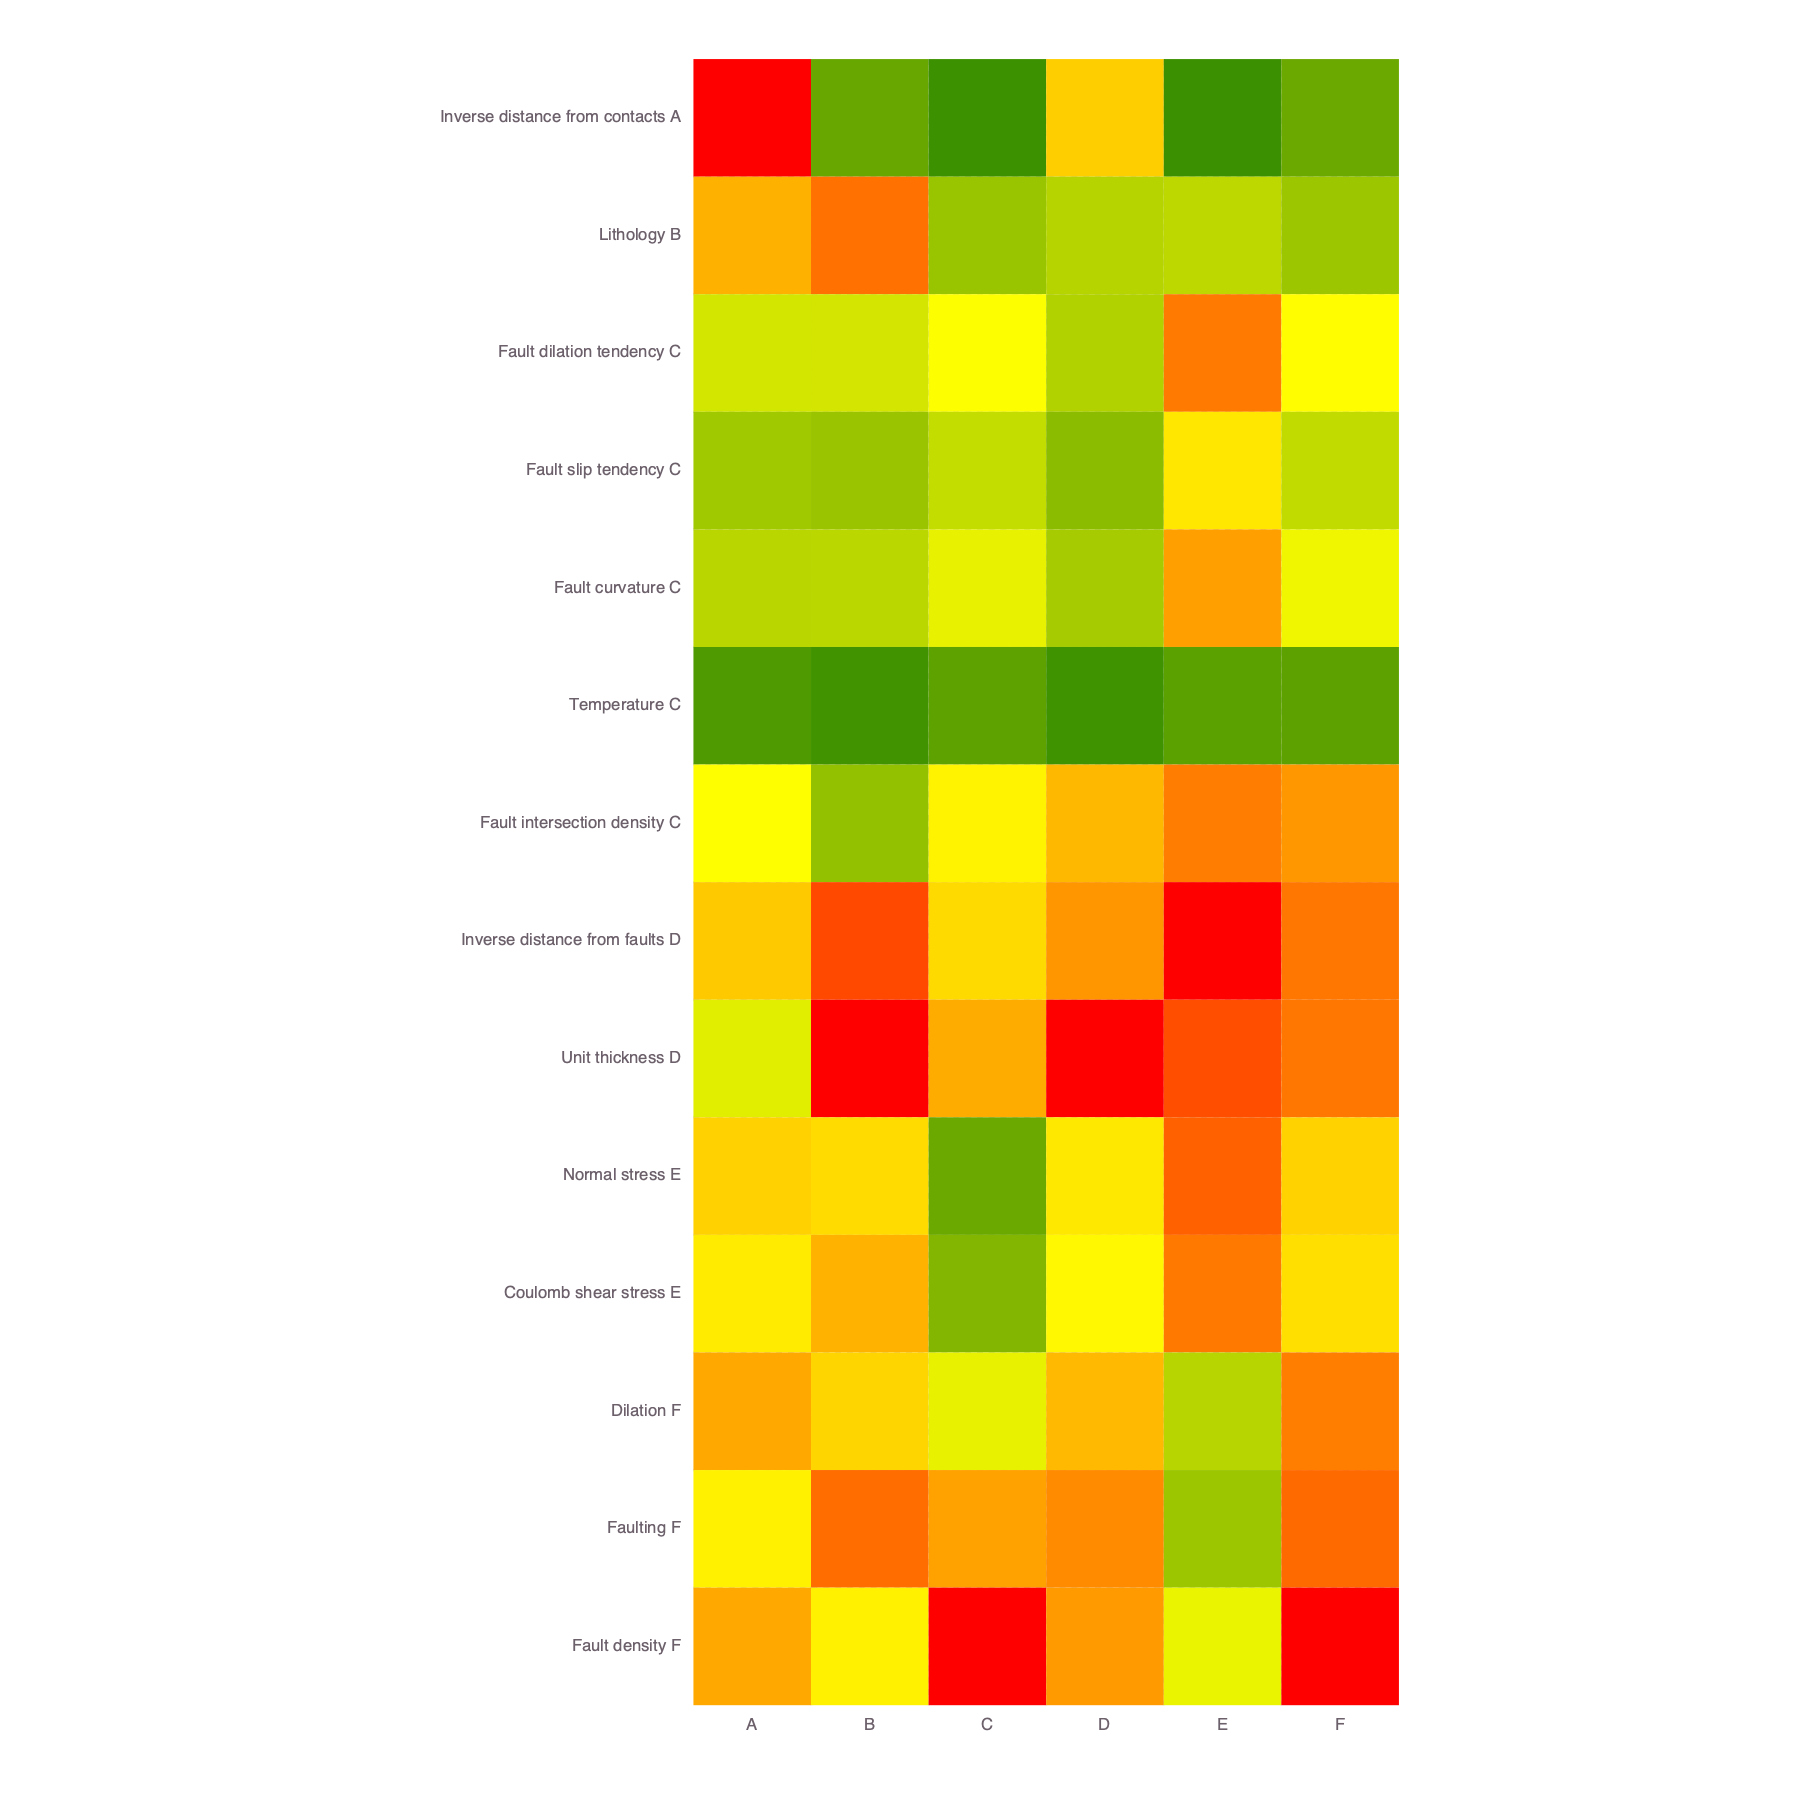
\includegraphics{../figures-set00-v9-inv-750-1000-daln/attributes-6-labeled-sorted.png}
\caption{attributes-6-labeled-sorted}
\end{figure}

Note that the attribute matrix \texttt{W} is automatically modified to
account that a range of vertical depths is applied in characterizing the
site wells.

The well locations are also clustered into \textbf{6} groups:

This grouping is based on analyses of the location matrix \texttt{H}:

\begin{figure}
\centering
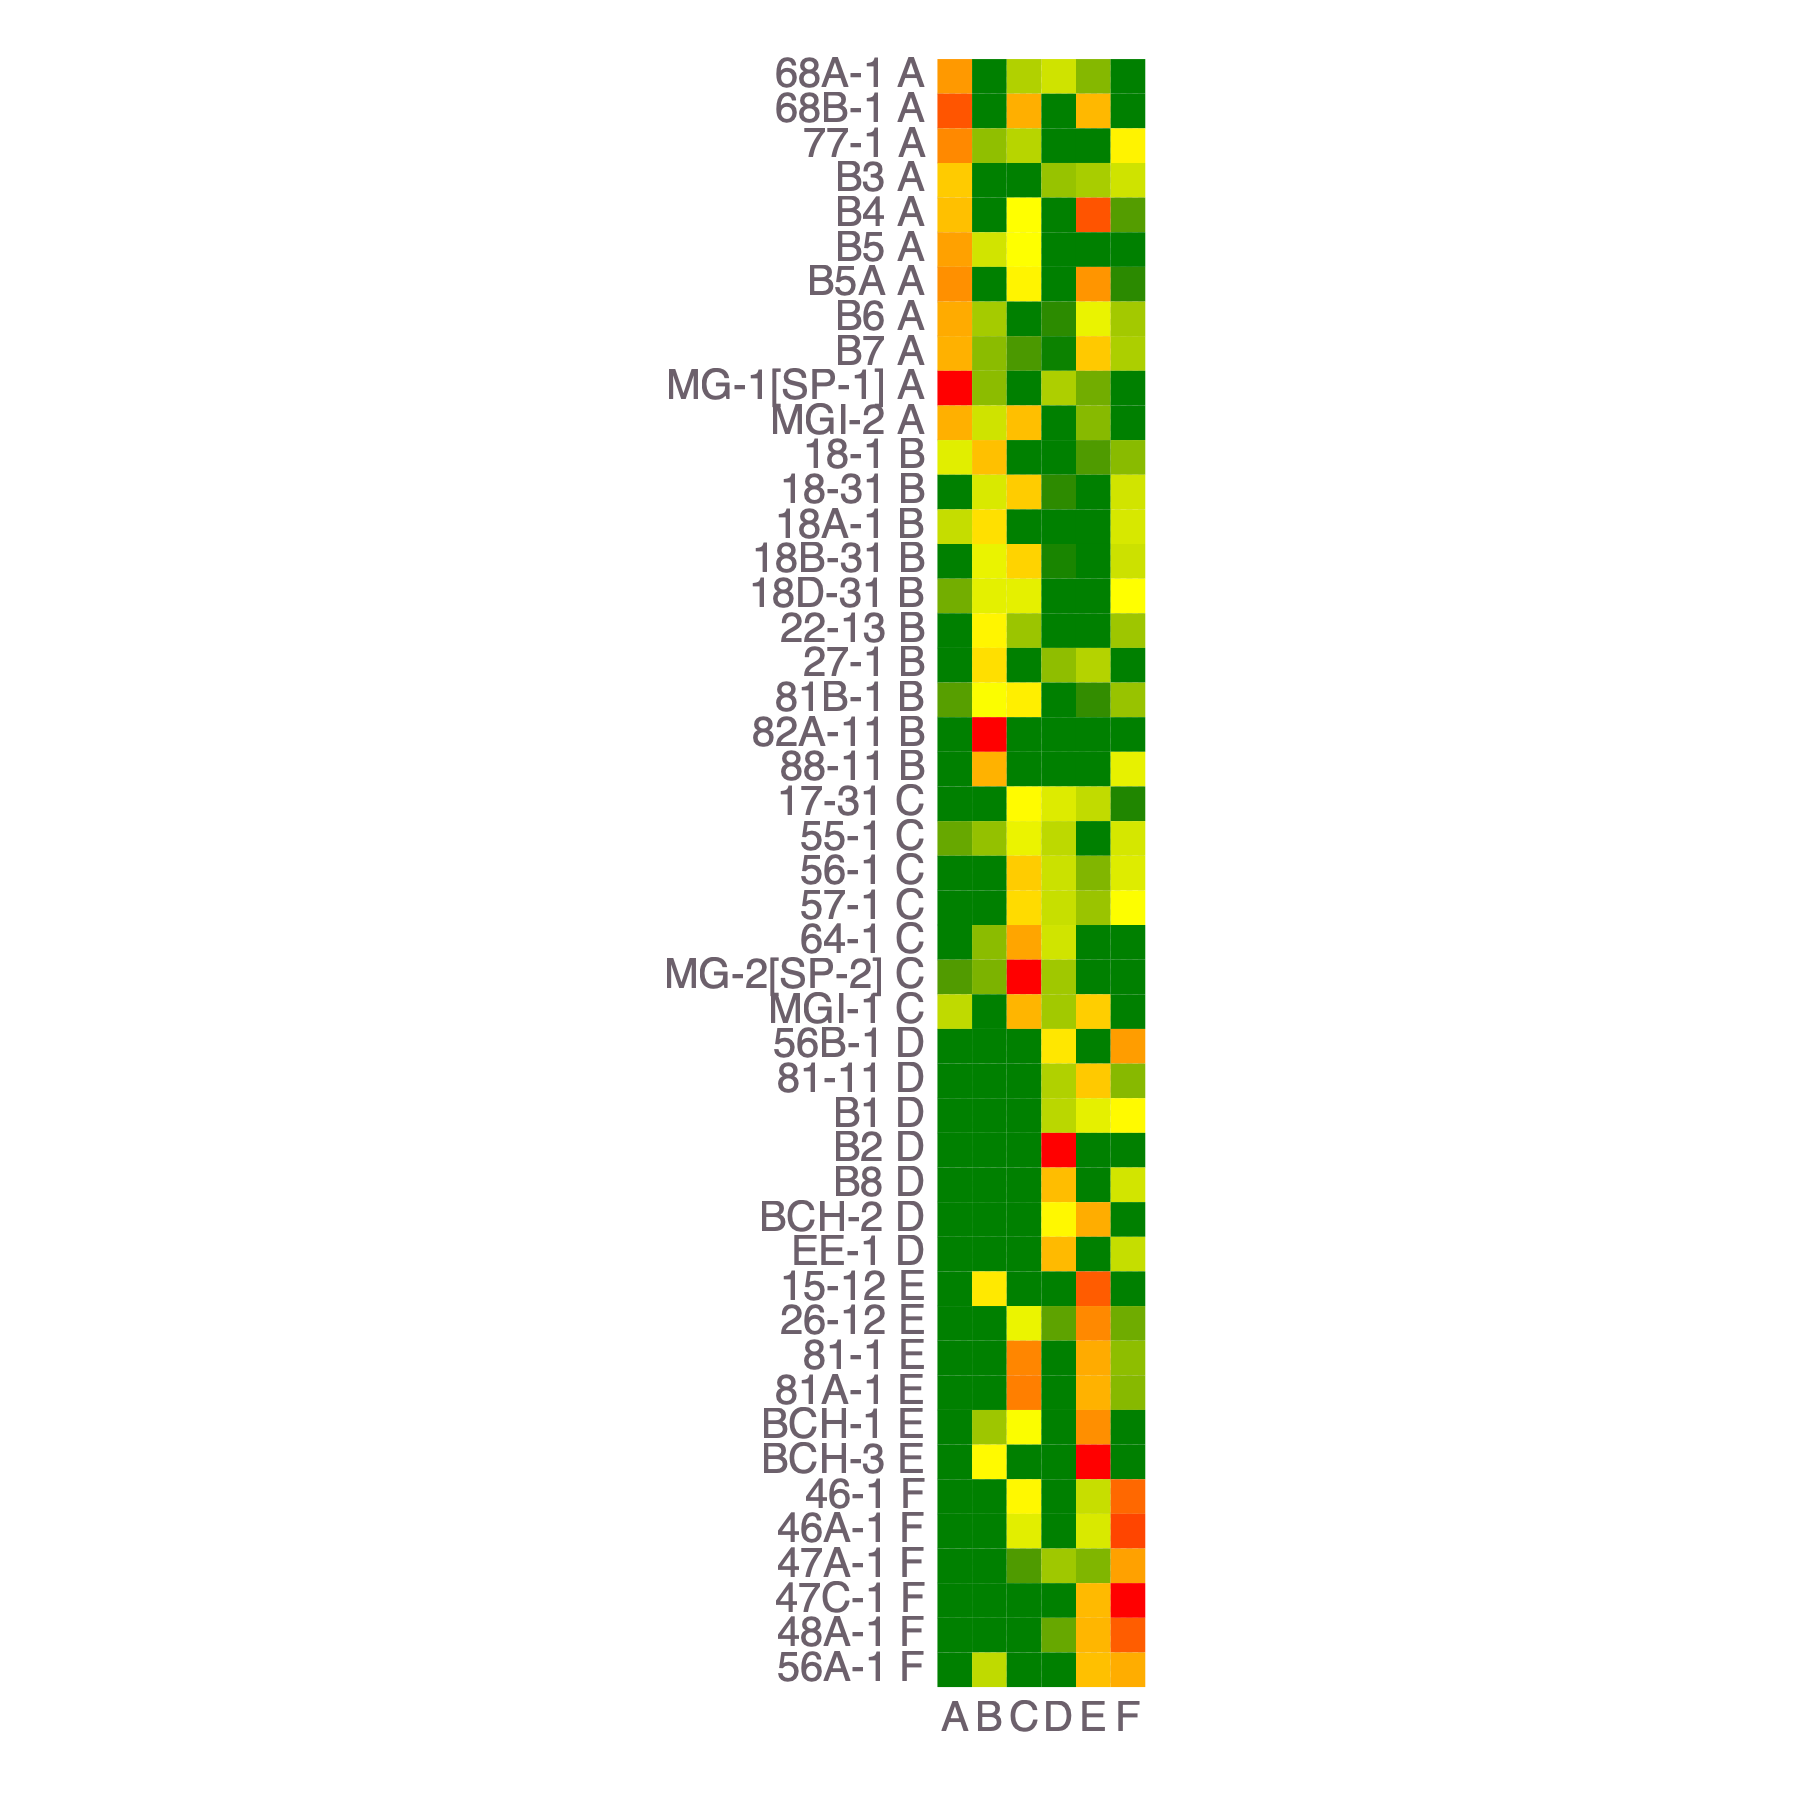
\includegraphics{../figures-set00-v9-inv-750-1000-daln/locations-6-labeled-sorted.png}
\caption{locations-6-labeled-sorted}
\end{figure}

The map \url{../figures-set00-v9-inv-750-1000-daln/locations-6-map.html}
provides interactive visualization of the extracted well location groups
(the html file can also be opened with any browser).

\begin{verbatim}
<iframe src="../figures-set00-v9-inv-750-1000-daln/locations-6-map.html" frameborder="0" height="400" width="50%"></iframe>
\end{verbatim}

More information on how the ML results are interpreted to provide
geothermal insights is discussed in our research paper.

    \hypertarget{type-2-flattening-focus-on-well-attributes}{%
\subsubsection{Type 2 flattening: Focus on well
attributes}\label{type-2-flattening-focus-on-well-attributes}}

\hypertarget{flatten-the-tensor-into-a-matrix}{%
\paragraph{Flatten the tensor into a
matrix}\label{flatten-the-tensor-into-a-matrix}}

    \begin{tcolorbox}[breakable, size=fbox, boxrule=1pt, pad at break*=1mm,colback=cellbackground, colframe=cellborder]
\prompt{In}{incolor}{23}{\boxspacing}
\begin{Verbatim}[commandchars=\\\{\}]
\PY{n}{Xdlan} \PY{o}{=} \PY{n}{reshape}\PY{p}{(}\PY{n}{permutedims}\PY{p}{(}\PY{n}{Tn}\PY{p}{,} \PY{p}{(}\PY{l+m+mi}{1}\PY{p}{,}\PY{l+m+mi}{3}\PY{p}{,}\PY{l+m+mi}{2}\PY{p}{)}\PY{p}{)}\PY{p}{,} \PY{p}{(}\PY{n}{depth} \PY{o}{*} \PY{n}{length}\PY{p}{(}\PY{n}{locations}\PY{p}{)}\PY{p}{)}\PY{p}{,} \PY{n}{length}\PY{p}{(}\PY{n}{attributes\PYZus{}process}\PY{p}{)}\PY{p}{)}\PY{p}{;}
\end{Verbatim}
\end{tcolorbox}

    Matrix rows merge the depth and well locations dimensions.

Matrix columns represent the well attributes.

    \hypertarget{perform-nmfk-analyses}{%
\paragraph{Perform NMFk analyses}\label{perform-nmfk-analyses}}

    \begin{tcolorbox}[breakable, size=fbox, boxrule=1pt, pad at break*=1mm,colback=cellbackground, colframe=cellborder]
\prompt{In}{incolor}{24}{\boxspacing}
\begin{Verbatim}[commandchars=\\\{\}]
\PY{n}{W}\PY{p}{,} \PY{n}{H}\PY{p}{,} \PY{n}{fitquality}\PY{p}{,} \PY{n}{robustness}\PY{p}{,} \PY{n}{aic} \PY{o}{=} \PY{n}{NMFk}\PY{o}{.}\PY{n}{execute}\PY{p}{(}\PY{n}{Xdlan}\PY{p}{,} \PY{n}{nkrange}\PY{p}{,} \PY{n}{nruns}\PY{p}{;} \PY{n}{resultdir}\PY{o}{=}\PY{n}{resultdir}\PY{p}{,} \PY{n}{casefilename}\PY{o}{=}\PY{l+s}{\PYZdq{}}\PY{l+s}{n}\PY{l+s}{m}\PY{l+s}{f}\PY{l+s}{k}\PY{l+s}{\PYZhy{}}\PY{l+s}{d}\PY{l+s}{l}\PY{l+s}{a}\PY{l+s}{n}\PY{l+s}{\PYZhy{}}\PY{l+s+si}{\PYZdl{}}\PY{p}{(}\PY{n}{join}\PY{p}{(}\PY{n}{size}\PY{p}{(}\PY{n}{Xdlan}\PY{p}{)}\PY{p}{,} \PY{l+s+sc}{\PYZsq{}\PYZus{}\PYZsq{}}\PY{p}{)}\PY{p}{)}\PY{l+s}{\PYZdq{}}\PY{p}{,} \PY{n}{load}\PY{o}{=}\PY{k+kc}{true}\PY{p}{)}
\PY{n}{W}\PY{p}{,} \PY{n}{H}\PY{p}{,} \PY{n}{fitquality}\PY{p}{,} \PY{n}{robustness}\PY{p}{,} \PY{n}{aic} \PY{o}{=} \PY{n}{NMFk}\PY{o}{.}\PY{n}{load}\PY{p}{(}\PY{n}{nkrange}\PY{p}{,} \PY{n}{nruns}\PY{p}{;} \PY{n}{resultdir}\PY{o}{=}\PY{n}{resultdir}\PY{p}{,} \PY{n}{casefilename}\PY{o}{=}\PY{l+s}{\PYZdq{}}\PY{l+s}{n}\PY{l+s}{m}\PY{l+s}{f}\PY{l+s}{k}\PY{l+s}{\PYZhy{}}\PY{l+s}{d}\PY{l+s}{l}\PY{l+s}{a}\PY{l+s}{n}\PY{l+s}{\PYZhy{}}\PY{l+s+si}{\PYZdl{}}\PY{p}{(}\PY{n}{join}\PY{p}{(}\PY{n}{size}\PY{p}{(}\PY{n}{Xdlan}\PY{p}{)}\PY{p}{,} \PY{l+s+sc}{\PYZsq{}\PYZus{}\PYZsq{}}\PY{p}{)}\PY{p}{)}\PY{l+s}{\PYZdq{}}\PY{p}{)}\PY{p}{;}
\end{Verbatim}
\end{tcolorbox}

    \begin{Verbatim}[commandchars=\\\{\}]
Signals:  2 Fit:     8717.101 Silhouette:    0.9918721 AIC:     -1087260
Signals:  3 Fit:     6319.428 Silhouette:    0.5782437 AIC:     -1124899
Signals:  4 Fit:     4843.099 Silhouette:   -0.2086358 AIC:     -1143846
Signals:  5 Fit:     3526.994 Silhouette:   0.03306949 AIC:     -1179956
Signals:  6 Fit:     2430.352 Silhouette:   -0.5717948 AIC:     -1234661
Signals:  7 Fit:     1649.869 Silhouette:   -0.4817311 AIC:     -1294388
Signals:  8 Fit:     1182.794 Silhouette:    0.1610176 AIC:     -1335780
Signals:  2 Fit:     8717.101 Silhouette:    0.9918721 AIC:     -1087260
Signals:  3 Fit:     6319.428 Silhouette:    0.5782437 AIC:     -1124899
Signals:  4 Fit:     4843.099 Silhouette:   -0.2086358 AIC:     -1143846
Signals:  5 Fit:     3526.994 Silhouette:   0.03306949 AIC:     -1179956
Signals:  6 Fit:     2430.352 Silhouette:   -0.5717948 AIC:     -1234661
Signals:  7 Fit:     1649.869 Silhouette:   -0.4817311 AIC:     -1294388
Signals:  8 Fit:     1182.794 Silhouette:    0.1610176 AIC:     -1335780
Signals:  2 Fit:     8717.101 Silhouette:    0.9918721 AIC:     -1087260
Signals:  3 Fit:     6319.428 Silhouette:    0.5782437 AIC:     -1124899
Signals:  4 Fit:     4843.099 Silhouette:   -0.2086358 AIC:     -1143846
Signals:  5 Fit:     3526.994 Silhouette:   0.03306949 AIC:     -1179956
Signals:  6 Fit:     2430.352 Silhouette:   -0.5717948 AIC:     -1234661
Signals:  7 Fit:     1649.869 Silhouette:   -0.4817311 AIC:     -1294388
Signals:  8 Fit:     1182.794 Silhouette:    0.1610176 AIC:     -1335780
┌ Info: Results
└ @ NMFk /Users/vvv/.julia/dev/NMFk/src/NMFkExecute.jl:15
┌ Info: Optimal solution: 3 signals
└ @ NMFk /Users/vvv/.julia/dev/NMFk/src/NMFkExecute.jl:20
┌ Info: Optimal solution: 3 signals
└ @ NMFk /Users/vvv/.julia/dev/NMFk/src/NMFkIO.jl:30
    \end{Verbatim}

    Here the \textbf{NMFk} results are loaded from a prior ML run.

As seen from the output above, the \textbf{NMFk} analyses identified
that the optimal number of geothermal signatures in the dataset
\textbf{3}.

Solutions with a number of signatures less than \textbf{3} are
underfitting.

Solutions with a number of signatures greater than \textbf{3} are
overfitting and unacceptable.

The set of acceptable solutions are defined by the \textbf{NMFk}
algorithm as follows:

    \begin{tcolorbox}[breakable, size=fbox, boxrule=1pt, pad at break*=1mm,colback=cellbackground, colframe=cellborder]
\prompt{In}{incolor}{25}{\boxspacing}
\begin{Verbatim}[commandchars=\\\{\}]
\PY{n}{NMFk}\PY{o}{.}\PY{n}{getks}\PY{p}{(}\PY{n}{nkrange}\PY{p}{,} \PY{n}{robustness}\PY{p}{[}\PY{n}{nkrange}\PY{p}{]}\PY{p}{)}
\end{Verbatim}
\end{tcolorbox}

            \begin{tcolorbox}[breakable, size=fbox, boxrule=.5pt, pad at break*=1mm, opacityfill=0]
\prompt{Out}{outcolor}{25}{\boxspacing}
\begin{Verbatim}[commandchars=\\\{\}]
2-element Array\{Int64,1\}:
 2
 3
\end{Verbatim}
\end{tcolorbox}
        
    The acceptable solutions contain 2 and 3 signatures.

    \hypertarget{post-process-nmfk-results}{%
\paragraph{Post-process NMFk results}\label{post-process-nmfk-results}}

\hypertarget{number-of-signatures}{%
\paragraph{Number of signatures}\label{number-of-signatures}}

Below is a plot representing solution quality (fit) and silhouette width
(robustness) for different numbers of signatures \texttt{k}:

    \begin{tcolorbox}[breakable, size=fbox, boxrule=1pt, pad at break*=1mm,colback=cellbackground, colframe=cellborder]
\prompt{In}{incolor}{26}{\boxspacing}
\begin{Verbatim}[commandchars=\\\{\}]
\PY{n}{NMFk}\PY{o}{.}\PY{n}{plot\PYZus{}signal\PYZus{}selecton}\PY{p}{(}\PY{n}{nkrange}\PY{p}{,} \PY{n}{fitquality}\PY{p}{,} \PY{n}{robustness}\PY{p}{;} \PY{n}{figuredir}\PY{o}{=}\PY{l+s}{\PYZdq{}}\PY{l+s+si}{\PYZdl{}figuredir}\PY{l+s}{\PYZhy{}}\PY{l+s+si}{\PYZdl{}}\PY{p}{(}\PY{n}{nruns}\PY{p}{)}\PY{l+s}{\PYZhy{}}\PY{l+s}{d}\PY{l+s}{l}\PY{l+s}{a}\PY{l+s}{n}\PY{l+s}{\PYZdq{}}\PY{p}{,} \PY{n}{xtitle}\PY{o}{=}\PY{l+s}{\PYZdq{}}\PY{l+s}{N}\PY{l+s}{u}\PY{l+s}{m}\PY{l+s}{b}\PY{l+s}{e}\PY{l+s}{r}\PY{l+s}{ }\PY{l+s}{o}\PY{l+s}{f}\PY{l+s}{ }\PY{l+s}{s}\PY{l+s}{i}\PY{l+s}{g}\PY{l+s}{n}\PY{l+s}{a}\PY{l+s}{t}\PY{l+s}{u}\PY{l+s}{r}\PY{l+s}{e}\PY{l+s}{s}\PY{l+s}{\PYZdq{}}\PY{p}{)}
\end{Verbatim}
\end{tcolorbox}

    \begin{center}
    \adjustimage{max size={0.9\linewidth}{0.9\paperheight}}{Brady_files/Brady_63_0.png}
    \end{center}
    { \hspace*{\fill} \\}
    
    \begin{Verbatim}[commandchars=\\\{\}]

    \end{Verbatim}

    The plot above also demonstrates that the acceptable solutions contain 2
and 3 signatures.

\hypertarget{analysis-of-all-the-acceptable-solutions}{%
\paragraph{Analysis of all the acceptable
solutions}\label{analysis-of-all-the-acceptable-solutions}}

The ML solutions containing an acceptable number of signatures are
further analyzed as follows:

    \begin{tcolorbox}[breakable, size=fbox, boxrule=1pt, pad at break*=1mm,colback=cellbackground, colframe=cellborder]
\prompt{In}{incolor}{27}{\boxspacing}
\begin{Verbatim}[commandchars=\\\{\}]
\PY{n}{NMFk}\PY{o}{.}\PY{n}{clusterresults}\PY{p}{(}\PY{n}{NMFk}\PY{o}{.}\PY{n}{getks}\PY{p}{(}\PY{n}{nkrange}\PY{p}{,} \PY{n}{robustness}\PY{p}{[}\PY{n}{nkrange}\PY{p}{]}\PY{p}{)}\PY{p}{,} \PY{n}{W}\PY{p}{,} \PY{n}{H}\PY{p}{,} \PY{n}{locations}\PY{p}{,} \PY{n}{attributes\PYZus{}process\PYZus{}long}\PY{p}{;} \PY{n}{loadassignements}\PY{o}{=}\PY{k+kc}{true}\PY{p}{,} \PY{n}{lon}\PY{o}{=}\PY{n}{xcoord}\PY{p}{,} \PY{n}{lat}\PY{o}{=}\PY{n}{ycoord}\PY{p}{,} \PY{n}{Wsize}\PY{o}{=}\PY{n}{depth}\PY{p}{,} \PY{n}{Wcasefilename}\PY{o}{=}\PY{l+s}{\PYZdq{}}\PY{l+s}{l}\PY{l+s}{o}\PY{l+s}{c}\PY{l+s}{a}\PY{l+s}{t}\PY{l+s}{i}\PY{l+s}{o}\PY{l+s}{n}\PY{l+s}{s}\PY{l+s}{\PYZdq{}}\PY{p}{,} \PY{n}{Hcasefilename}\PY{o}{=}\PY{l+s}{\PYZdq{}}\PY{l+s}{a}\PY{l+s}{t}\PY{l+s}{t}\PY{l+s}{r}\PY{l+s}{i}\PY{l+s}{b}\PY{l+s}{u}\PY{l+s}{t}\PY{l+s}{e}\PY{l+s}{s}\PY{l+s}{\PYZdq{}}\PY{p}{,} \PY{n}{resultdir}\PY{o}{=}\PY{n}{resultdir} \PY{o}{*} \PY{l+s}{\PYZdq{}}\PY{l+s}{\PYZhy{}}\PY{l+s+si}{\PYZdl{}}\PY{p}{(}\PY{n}{nruns}\PY{p}{)}\PY{l+s}{\PYZhy{}}\PY{l+s}{d}\PY{l+s}{l}\PY{l+s}{a}\PY{l+s}{n}\PY{l+s}{\PYZdq{}}\PY{p}{,} \PY{n}{figuredir}\PY{o}{=}\PY{n}{figuredir} \PY{o}{*} \PY{l+s}{\PYZdq{}}\PY{l+s}{\PYZhy{}}\PY{l+s+si}{\PYZdl{}}\PY{p}{(}\PY{n}{nruns}\PY{p}{)}\PY{l+s}{\PYZhy{}}\PY{l+s}{d}\PY{l+s}{l}\PY{l+s}{a}\PY{l+s}{n}\PY{l+s}{\PYZdq{}}\PY{p}{,} \PY{n}{hover}\PY{o}{=}\PY{l+s}{\PYZdq{}}\PY{l+s}{W}\PY{l+s}{e}\PY{l+s}{l}\PY{l+s}{l}\PY{l+s}{:}\PY{l+s}{ }\PY{l+s}{\PYZdq{}} \PY{o}{.*} \PY{n}{locations} \PY{o}{.*} \PY{l+s}{\PYZdq{}}\PY{l+s}{\PYZlt{}}\PY{l+s}{b}\PY{l+s}{r}\PY{l+s}{\PYZgt{}}\PY{l+s}{\PYZdq{}} \PY{o}{.*} \PY{l+s}{\PYZdq{}}\PY{l+s}{W}\PY{l+s}{e}\PY{l+s}{l}\PY{l+s}{l}\PY{l+s}{T}\PY{l+s}{y}\PY{l+s}{p}\PY{l+s}{e}\PY{l+s}{:}\PY{l+s}{ }\PY{l+s}{\PYZdq{}} \PY{o}{.*} \PY{n}{String}\PY{o}{.}\PY{p}{(}\PY{n}{welltype}\PY{p}{)} \PY{o}{.*} \PY{l+s}{\PYZdq{}}\PY{l+s}{\PYZlt{}}\PY{l+s}{b}\PY{l+s}{r}\PY{l+s}{\PYZgt{}}\PY{l+s}{\PYZdq{}} \PY{o}{.*} \PY{n}{production}\PY{p}{,} \PY{n}{Wmatrix\PYZus{}font\PYZus{}size}\PY{o}{=}\PY{l+m+mi}{4}\PY{n}{Gadfly}\PY{o}{.}\PY{n}{pt}\PY{p}{,} \PY{n}{biplotcolor}\PY{o}{=}\PY{o}{:}\PY{n}{WH}\PY{p}{,} \PY{n}{biplotlabel}\PY{o}{=}\PY{o}{:}\PY{n}{WH}\PY{p}{)}
\end{Verbatim}
\end{tcolorbox}

    \begin{Verbatim}[commandchars=\\\{\}]
Signal importance (high->low): [2, 1]
┌ Info: Number of signals: 2
└ @ NMFk /Users/vvv/.julia/dev/NMFk/src/NMFkPostprocess.jl:144
┌ Info: Attributes (signals=2)
└ @ NMFk /Users/vvv/.julia/dev/NMFk/src/NMFkPostprocess.jl:148
┌ Warning: type
Clustering.KmeansResult\{Core.Array\{Core.Float64,2\},Core.Float64,Core.Int64\} not
present in workspace; reconstructing
└ @ JLD /Users/vvv/.julia/packages/JLD/nQ9iW/src/jld\_types.jl:697
┌ Info: Robust k-means analysis results are loaded from file results-
set00-v9-inv-750-1000-dlan/Hmatrix-2-2\_14-1000.jld!
└ @ NMFk /Users/vvv/.julia/dev/NMFk/src/NMFkCluster.jl:67
┌ Warning: Procedure to find unique signals could not identify a solution {\ldots}
└ @ NMFk /Users/vvv/.julia/dev/NMFk/src/NMFkCluster.jl:158
┌ Warning: Procedure to find unique signals could not identify a solution {\ldots}
└ @ NMFk /Users/vvv/.julia/dev/NMFk/src/NMFkCluster.jl:158
┌ Warning: type
Clustering.KmeansResult\{Core.Array\{Core.Float64,2\},Core.Float64,Core.Int64\} not
present in workspace; reconstructing
└ @ JLD /Users/vvv/.julia/packages/JLD/nQ9iW/src/jld\_types.jl:697
    \end{Verbatim}

    
    \begin{Verbatim}[commandchars=\\\{\}]
10×2 Array\{Any,2\}:
 "Unit thickness"                  1.0
 "Faulting"                        0.863986
 "Fault density"                   0.849999
 "Inverse distance from faults"    0.792619
 "Dilation"                        0.75876
 "Normal stress"                   0.674322
 "Fault intersection density"      0.673763
 "Coulomb shear stress"            0.672813
 "Lithology"                       0.501336
 "Inverse distance from contacts"  0.388519
    \end{Verbatim}

    
    
    \begin{Verbatim}[commandchars=\\\{\}]
4×2 Array\{Any,2\}:
 "Fault dilation tendency"  1.0
 "Fault curvature"          0.89069
 "Fault slip tendency"      0.706146
 "Temperature"              0.239306
    \end{Verbatim}

    
    \begin{center}
    \adjustimage{max size={0.9\linewidth}{0.9\paperheight}}{Brady_files/Brady_65_3.png}
    \end{center}
    { \hspace*{\fill} \\}
    
    \begin{Verbatim}[commandchars=\\\{\}]
┌ Info: Robust k-means analysis results are loaded from file results-
set00-v9-inv-750-1000-dlan/Wmatrix-2-2\_47-1000.jld!
└ @ NMFk /Users/vvv/.julia/dev/NMFk/src/NMFkCluster.jl:67
┌ Warning: Procedure to find unique signals could not identify a solution {\ldots}
└ @ NMFk /Users/vvv/.julia/dev/NMFk/src/NMFkCluster.jl:158
┌ Warning: Procedure to find unique signals could not identify a solution {\ldots}
└ @ NMFk /Users/vvv/.julia/dev/NMFk/src/NMFkCluster.jl:158
┌ Info: Signal A -> A Count: 10
└ @ NMFk /Users/vvv/.julia/dev/NMFk/src/NMFkPostprocess.jl:255
┌ Info: Signal B -> B Count: 4
└ @ NMFk /Users/vvv/.julia/dev/NMFk/src/NMFkPostprocess.jl:255
┌ Info: Signal A (S2) (k-means clustering)
└ @ NMFk /Users/vvv/.julia/dev/NMFk/src/NMFkPostprocess.jl:272
┌ Info: Signal B (S1) (k-means clustering)
└ @ NMFk /Users/vvv/.julia/dev/NMFk/src/NMFkPostprocess.jl:272
    \end{Verbatim}

    \begin{center}
    \adjustimage{max size={0.9\linewidth}{0.9\paperheight}}{Brady_files/Brady_65_5.png}
    \end{center}
    { \hspace*{\fill} \\}
    
    \begin{Verbatim}[commandchars=\\\{\}]

    \end{Verbatim}

    \begin{center}
    \adjustimage{max size={0.9\linewidth}{0.9\paperheight}}{Brady_files/Brady_65_7.png}
    \end{center}
    { \hspace*{\fill} \\}
    
    \begin{center}
    \adjustimage{max size={0.9\linewidth}{0.9\paperheight}}{Brady_files/Brady_65_8.png}
    \end{center}
    { \hspace*{\fill} \\}
    
    \begin{Verbatim}[commandchars=\\\{\}]

    \end{Verbatim}

    \begin{center}
    \adjustimage{max size={0.9\linewidth}{0.9\paperheight}}{Brady_files/Brady_65_10.png}
    \end{center}
    { \hspace*{\fill} \\}
    
    
    \begin{Verbatim}[commandchars=\\\{\}]
27×2 Array\{Any,2\}:
 "B8"          1.0
 "EE-1"        0.998613
 "MG-1(SP-1)"  0.956943
 "68A-1"       0.916159
 "64-1"        0.864026
 "47A-1"       0.859446
 "77-1"        0.857345
 "MG-2(SP-2)"  0.853707
 "27-1"        0.829554
 "82A-11"      0.807563
 "18A-1"       0.782265
 "47C-1"       0.745002
 "22-13"       0.734719
 ⋮             
 "88-11"       0.659403
 "46A-1"       0.629757
 "B5"          0.614479
 "46-1"        0.594959
 "48A-1"       0.590979
 "B1"          0.501909
 "56B-1"       0.497064
 "26-12"       0.472464
 "81-11"       0.416937
 "MGI-1"       0.24275
 "B3"          0.241753
 "B2"          0.127328
    \end{Verbatim}

    
    
    \begin{Verbatim}[commandchars=\\\{\}]
20×2 Array\{Any,2\}:
 "56-1"    1.0
 "55-1"    0.949937
 "57-1"    0.947965
 "BCH-3"   0.872622
 "15-12"   0.808709
 "68B-1"   0.758469
 "56A-1"   0.753147
 "BCH-1"   0.608981
 "B5A"     0.43926
 "17-31"   0.366493
 "18B-31"  0.348668
 "81B-1"   0.320223
 "18D-31"  0.298697
 "MGI-2"   0.291839
 "B4"      0.286734
 "18-31"   0.260379
 "B6"      0.257226
 "81-1"    0.234119
 "81A-1"   0.207054
 "B7"      0.156777
    \end{Verbatim}

    
    \begin{center}
    \adjustimage{max size={0.9\linewidth}{0.9\paperheight}}{Brady_files/Brady_65_13.png}
    \end{center}
    { \hspace*{\fill} \\}
    
    \begin{Verbatim}[commandchars=\\\{\}]
┌ Info: Locations (signals=2)
└ @ NMFk /Users/vvv/.julia/dev/NMFk/src/NMFkPostprocess.jl:322
┌ Info: Signal A (S2) Count: 27
└ @ NMFk /Users/vvv/.julia/dev/NMFk/src/NMFkPostprocess.jl:335
┌ Info: Signal B (S1) Count: 20
└ @ NMFk /Users/vvv/.julia/dev/NMFk/src/NMFkPostprocess.jl:335
┌ Info: Signal A -> A Count: 27
└ @ NMFk /Users/vvv/.julia/dev/NMFk/src/NMFkPostprocess.jl:345
┌ Info: Signal B -> B Count: 20
└ @ NMFk /Users/vvv/.julia/dev/NMFk/src/NMFkPostprocess.jl:345
┌ Info: Signal A (remapped k-means clustering)
└ @ NMFk /Users/vvv/.julia/dev/NMFk/src/NMFkPostprocess.jl:360
┌ Info: Signal B (remapped k-means clustering)
└ @ NMFk /Users/vvv/.julia/dev/NMFk/src/NMFkPostprocess.jl:360
    \end{Verbatim}

    \begin{center}
    \adjustimage{max size={0.9\linewidth}{0.9\paperheight}}{Brady_files/Brady_65_15.png}
    \end{center}
    { \hspace*{\fill} \\}
    
    \begin{Verbatim}[commandchars=\\\{\}]

    \end{Verbatim}

    \begin{center}
    \adjustimage{max size={0.9\linewidth}{0.9\paperheight}}{Brady_files/Brady_65_17.png}
    \end{center}
    { \hspace*{\fill} \\}
    
    \begin{center}
    \adjustimage{max size={0.9\linewidth}{0.9\paperheight}}{Brady_files/Brady_65_18.png}
    \end{center}
    { \hspace*{\fill} \\}
    
    \begin{Verbatim}[commandchars=\\\{\}]

    \end{Verbatim}

    \begin{center}
    \adjustimage{max size={0.9\linewidth}{0.9\paperheight}}{Brady_files/Brady_65_20.png}
    \end{center}
    { \hspace*{\fill} \\}
    
    \begin{center}
    \adjustimage{max size={0.9\linewidth}{0.9\paperheight}}{Brady_files/Brady_65_21.png}
    \end{center}
    { \hspace*{\fill} \\}
    
    \begin{Verbatim}[commandchars=\\\{\}]

    \end{Verbatim}

    \begin{center}
    \adjustimage{max size={0.9\linewidth}{0.9\paperheight}}{Brady_files/Brady_65_23.png}
    \end{center}
    { \hspace*{\fill} \\}
    
    \begin{Verbatim}[commandchars=\\\{\}]
Signal importance (high->low): [3, 1, 2]
┌ Info: Number of signals: 3
└ @ NMFk /Users/vvv/.julia/dev/NMFk/src/NMFkPostprocess.jl:144
┌ Info: Attributes (signals=3)
└ @ NMFk /Users/vvv/.julia/dev/NMFk/src/NMFkPostprocess.jl:148
┌ Warning: type
Clustering.KmeansResult\{Core.Array\{Core.Float64,2\},Core.Float64,Core.Int64\} not
present in workspace; reconstructing
└ @ JLD /Users/vvv/.julia/packages/JLD/nQ9iW/src/jld\_types.jl:697
┌ Info: Robust k-means analysis results are loaded from file results-
set00-v9-inv-750-1000-dlan/Hmatrix-3-3\_14-1000.jld!
└ @ NMFk /Users/vvv/.julia/dev/NMFk/src/NMFkCluster.jl:67
┌ Warning: Procedure to find unique signals could not identify a solution {\ldots}
└ @ NMFk /Users/vvv/.julia/dev/NMFk/src/NMFkCluster.jl:158
┌ Warning: Procedure to find unique signals could not identify a solution {\ldots}
└ @ NMFk /Users/vvv/.julia/dev/NMFk/src/NMFkCluster.jl:158
┌ Warning: Procedure to find unique signals could not identify a solution {\ldots}
└ @ NMFk /Users/vvv/.julia/dev/NMFk/src/NMFkCluster.jl:158
┌ Warning: type
Clustering.KmeansResult\{Core.Array\{Core.Float64,2\},Core.Float64,Core.Int64\} not
present in workspace; reconstructing
└ @ JLD /Users/vvv/.julia/packages/JLD/nQ9iW/src/jld\_types.jl:697
┌ Info: Robust k-means analysis results are loaded from file results-
set00-v9-inv-750-1000-dlan/Wmatrix-3-3\_47-1000.jld!
└ @ NMFk /Users/vvv/.julia/dev/NMFk/src/NMFkCluster.jl:67
    \end{Verbatim}

    
    \begin{Verbatim}[commandchars=\\\{\}]
9×2 Array\{Any,2\}:
 "Unit thickness"                  1.0
 "Faulting"                        0.703863
 "Dilation"                        0.652914
 "Inverse distance from faults"    0.645557
 "Fault density"                   0.641279
 "Fault intersection density"      0.633706
 "Normal stress"                   0.558339
 "Coulomb shear stress"            0.544241
 "Inverse distance from contacts"  0.377979
    \end{Verbatim}

    
    
    \begin{Verbatim}[commandchars=\\\{\}]
4×2 Array\{Any,2\}:
 "Fault dilation tendency"  1.0
 "Fault curvature"          0.89069
 "Fault slip tendency"      0.706146
 "Temperature"              0.239306
    \end{Verbatim}

    
    
    \begin{Verbatim}[commandchars=\\\{\}]
1×2 Array\{Any,2\}:
 "Lithology"  1.0
    \end{Verbatim}

    
    \begin{center}
    \adjustimage{max size={0.9\linewidth}{0.9\paperheight}}{Brady_files/Brady_65_28.png}
    \end{center}
    { \hspace*{\fill} \\}
    
    \begin{Verbatim}[commandchars=\\\{\}]
┌ Warning: Procedure to find unique signals could not identify a solution {\ldots}
└ @ NMFk /Users/vvv/.julia/dev/NMFk/src/NMFkCluster.jl:158
┌ Info: Signal A -> A Count: 9
└ @ NMFk /Users/vvv/.julia/dev/NMFk/src/NMFkPostprocess.jl:255
┌ Info: Signal B -> B Count: 4
└ @ NMFk /Users/vvv/.julia/dev/NMFk/src/NMFkPostprocess.jl:255
┌ Info: Signal C -> C Count: 1
└ @ NMFk /Users/vvv/.julia/dev/NMFk/src/NMFkPostprocess.jl:255
┌ Info: Signal A (S3) (k-means clustering)
└ @ NMFk /Users/vvv/.julia/dev/NMFk/src/NMFkPostprocess.jl:272
┌ Info: Signal B (S2) (k-means clustering)
└ @ NMFk /Users/vvv/.julia/dev/NMFk/src/NMFkPostprocess.jl:272
┌ Info: Signal C (S1) (k-means clustering)
└ @ NMFk /Users/vvv/.julia/dev/NMFk/src/NMFkPostprocess.jl:272
    \end{Verbatim}

    \begin{center}
    \adjustimage{max size={0.9\linewidth}{0.9\paperheight}}{Brady_files/Brady_65_30.png}
    \end{center}
    { \hspace*{\fill} \\}
    
    \begin{Verbatim}[commandchars=\\\{\}]

    \end{Verbatim}

    \begin{center}
    \adjustimage{max size={0.9\linewidth}{0.9\paperheight}}{Brady_files/Brady_65_32.png}
    \end{center}
    { \hspace*{\fill} \\}
    
    \begin{center}
    \adjustimage{max size={0.9\linewidth}{0.9\paperheight}}{Brady_files/Brady_65_33.png}
    \end{center}
    { \hspace*{\fill} \\}
    
    \begin{Verbatim}[commandchars=\\\{\}]

    \end{Verbatim}

    \begin{center}
    \adjustimage{max size={0.9\linewidth}{0.9\paperheight}}{Brady_files/Brady_65_35.png}
    \end{center}
    { \hspace*{\fill} \\}
    
    \begin{Verbatim}[commandchars=\\\{\}]

    \end{Verbatim}

    
    \begin{Verbatim}[commandchars=\\\{\}]
13×2 Array\{Any,2\}:
 "B8"     1.0
 "EE-1"   0.988215
 "47A-1"  0.905634
 "64-1"   0.867431
 "47C-1"  0.79874
 "27-1"   0.716696
 "46A-1"  0.699196
 "46-1"   0.675645
 "48A-1"  0.56726
 "56B-1"  0.557649
 "MGI-1"  0.286221
 "81A-1"  0.24804
 "B2"     0.0820308
    \end{Verbatim}

    
    
    \begin{Verbatim}[commandchars=\\\{\}]
20×2 Array\{Any,2\}:
 "56-1"        1.0
 "55-1"        0.951665
 "57-1"        0.947671
 "68B-1"       0.759123
 "56A-1"       0.752345
 "BCH-2"       0.67324
 "MG-2(SP-2)"  0.624464
 "BCH-1"       0.609265
 "B5A"         0.440143
 "B5"          0.439178
 "17-31"       0.372325
 "81-11"       0.353316
 "18B-31"      0.351038
 "81B-1"       0.32106
 "18D-31"      0.302397
 "MGI-2"       0.289056
 "B4"          0.286007
 "18-31"       0.261958
 "81-1"        0.234893
 "B7"          0.155895
    \end{Verbatim}

    
    
    \begin{Verbatim}[commandchars=\\\{\}]
14×2 Array\{Any,2\}:
 "88-11"       1.0
 "22-13"       0.890617
 "82A-11"      0.886939
 "68A-1"       0.878252
 "18-1"        0.872381
 "77-1"        0.834481
 "18A-1"       0.830688
 "MG-1(SP-1)"  0.807444
 "BCH-3"       0.805676
 "15-12"       0.791843
 "B1"          0.65222
 "26-12"       0.444381
 "B6"          0.213355
 "B3"          0.212844
    \end{Verbatim}

    
    \begin{center}
    \adjustimage{max size={0.9\linewidth}{0.9\paperheight}}{Brady_files/Brady_65_40.png}
    \end{center}
    { \hspace*{\fill} \\}
    
    \begin{Verbatim}[commandchars=\\\{\}]
┌ Info: Locations (signals=3)
└ @ NMFk /Users/vvv/.julia/dev/NMFk/src/NMFkPostprocess.jl:322
┌ Info: Signal A (S2) Count: 20
└ @ NMFk /Users/vvv/.julia/dev/NMFk/src/NMFkPostprocess.jl:335
┌ Info: Signal B (S1) Count: 14
└ @ NMFk /Users/vvv/.julia/dev/NMFk/src/NMFkPostprocess.jl:335
┌ Info: Signal C (S3) Count: 13
└ @ NMFk /Users/vvv/.julia/dev/NMFk/src/NMFkPostprocess.jl:335
┌ Info: Signal C -> A Count: 13
└ @ NMFk /Users/vvv/.julia/dev/NMFk/src/NMFkPostprocess.jl:345
┌ Info: Signal A -> B Count: 20
└ @ NMFk /Users/vvv/.julia/dev/NMFk/src/NMFkPostprocess.jl:345
┌ Info: Signal B -> C Count: 14
└ @ NMFk /Users/vvv/.julia/dev/NMFk/src/NMFkPostprocess.jl:345
┌ Info: Signal A (remapped k-means clustering)
└ @ NMFk /Users/vvv/.julia/dev/NMFk/src/NMFkPostprocess.jl:360
┌ Info: Signal B (remapped k-means clustering)
└ @ NMFk /Users/vvv/.julia/dev/NMFk/src/NMFkPostprocess.jl:360
┌ Info: Signal C (remapped k-means clustering)
└ @ NMFk /Users/vvv/.julia/dev/NMFk/src/NMFkPostprocess.jl:360
    \end{Verbatim}

    \begin{center}
    \adjustimage{max size={0.9\linewidth}{0.9\paperheight}}{Brady_files/Brady_65_42.png}
    \end{center}
    { \hspace*{\fill} \\}
    
    \begin{Verbatim}[commandchars=\\\{\}]

    \end{Verbatim}

    \begin{center}
    \adjustimage{max size={0.9\linewidth}{0.9\paperheight}}{Brady_files/Brady_65_44.png}
    \end{center}
    { \hspace*{\fill} \\}
    
    \begin{center}
    \adjustimage{max size={0.9\linewidth}{0.9\paperheight}}{Brady_files/Brady_65_45.png}
    \end{center}
    { \hspace*{\fill} \\}
    
    \begin{Verbatim}[commandchars=\\\{\}]

    \end{Verbatim}

    \begin{center}
    \adjustimage{max size={0.9\linewidth}{0.9\paperheight}}{Brady_files/Brady_65_47.png}
    \end{center}
    { \hspace*{\fill} \\}
    
    \begin{center}
    \adjustimage{max size={0.9\linewidth}{0.9\paperheight}}{Brady_files/Brady_65_48.png}
    \end{center}
    { \hspace*{\fill} \\}
    
    \begin{Verbatim}[commandchars=\\\{\}]

    \end{Verbatim}

    \begin{center}
    \adjustimage{max size={0.9\linewidth}{0.9\paperheight}}{Brady_files/Brady_65_50.png}
    \end{center}
    { \hspace*{\fill} \\}
    
    \begin{Verbatim}[commandchars=\\\{\}]

    \end{Verbatim}

            \begin{tcolorbox}[breakable, size=fbox, boxrule=.5pt, pad at break*=1mm, opacityfill=0]
\prompt{Out}{outcolor}{27}{\boxspacing}
\begin{Verbatim}[commandchars=\\\{\}]
([[2, 1], [3, 2, 1]], [['B', 'B', 'A', 'B', 'A', 'B', 'B', 'A', 'A', 'A'  …
'B', 'A', 'B', 'A', 'B', 'A', 'A', 'A', 'A', 'B'], ['C', 'B', 'C', 'B', 'C',
'B', 'B', 'C', 'C', 'A'  …  'B', 'A', 'B', 'B', 'C', 'A', 'C', 'B', 'A', 'B']],
[['A', 'A', 'A', 'A', 'B', 'B', 'B', 'B', 'A', 'A', 'A', 'A', 'A', 'A'], ['A',
'A', 'A', 'A', 'B', 'B', 'B', 'B', 'A', 'A', 'A', 'A', 'A', 'C']])
\end{Verbatim}
\end{tcolorbox}
        
    \hypertarget{analysis-of-the-3-signature-solution}{%
\paragraph{Analysis of the 3-signature
solution}\label{analysis-of-the-3-signature-solution}}

The results for a solution with \textbf{3} signatures presented above
will be further discussed here.

The well attributes are clustered into \textbf{3} groups:

\begin{verbatim}
<iframe src="../results-set00-v9-inv-750-1000-dlan/attributes-3-groups.txt" frameborder="0" height="400"
  width="95%"></iframe>
\end{verbatim}

This grouping is based on analyses of the attribute matrix \texttt{W}:

\begin{figure}
\centering
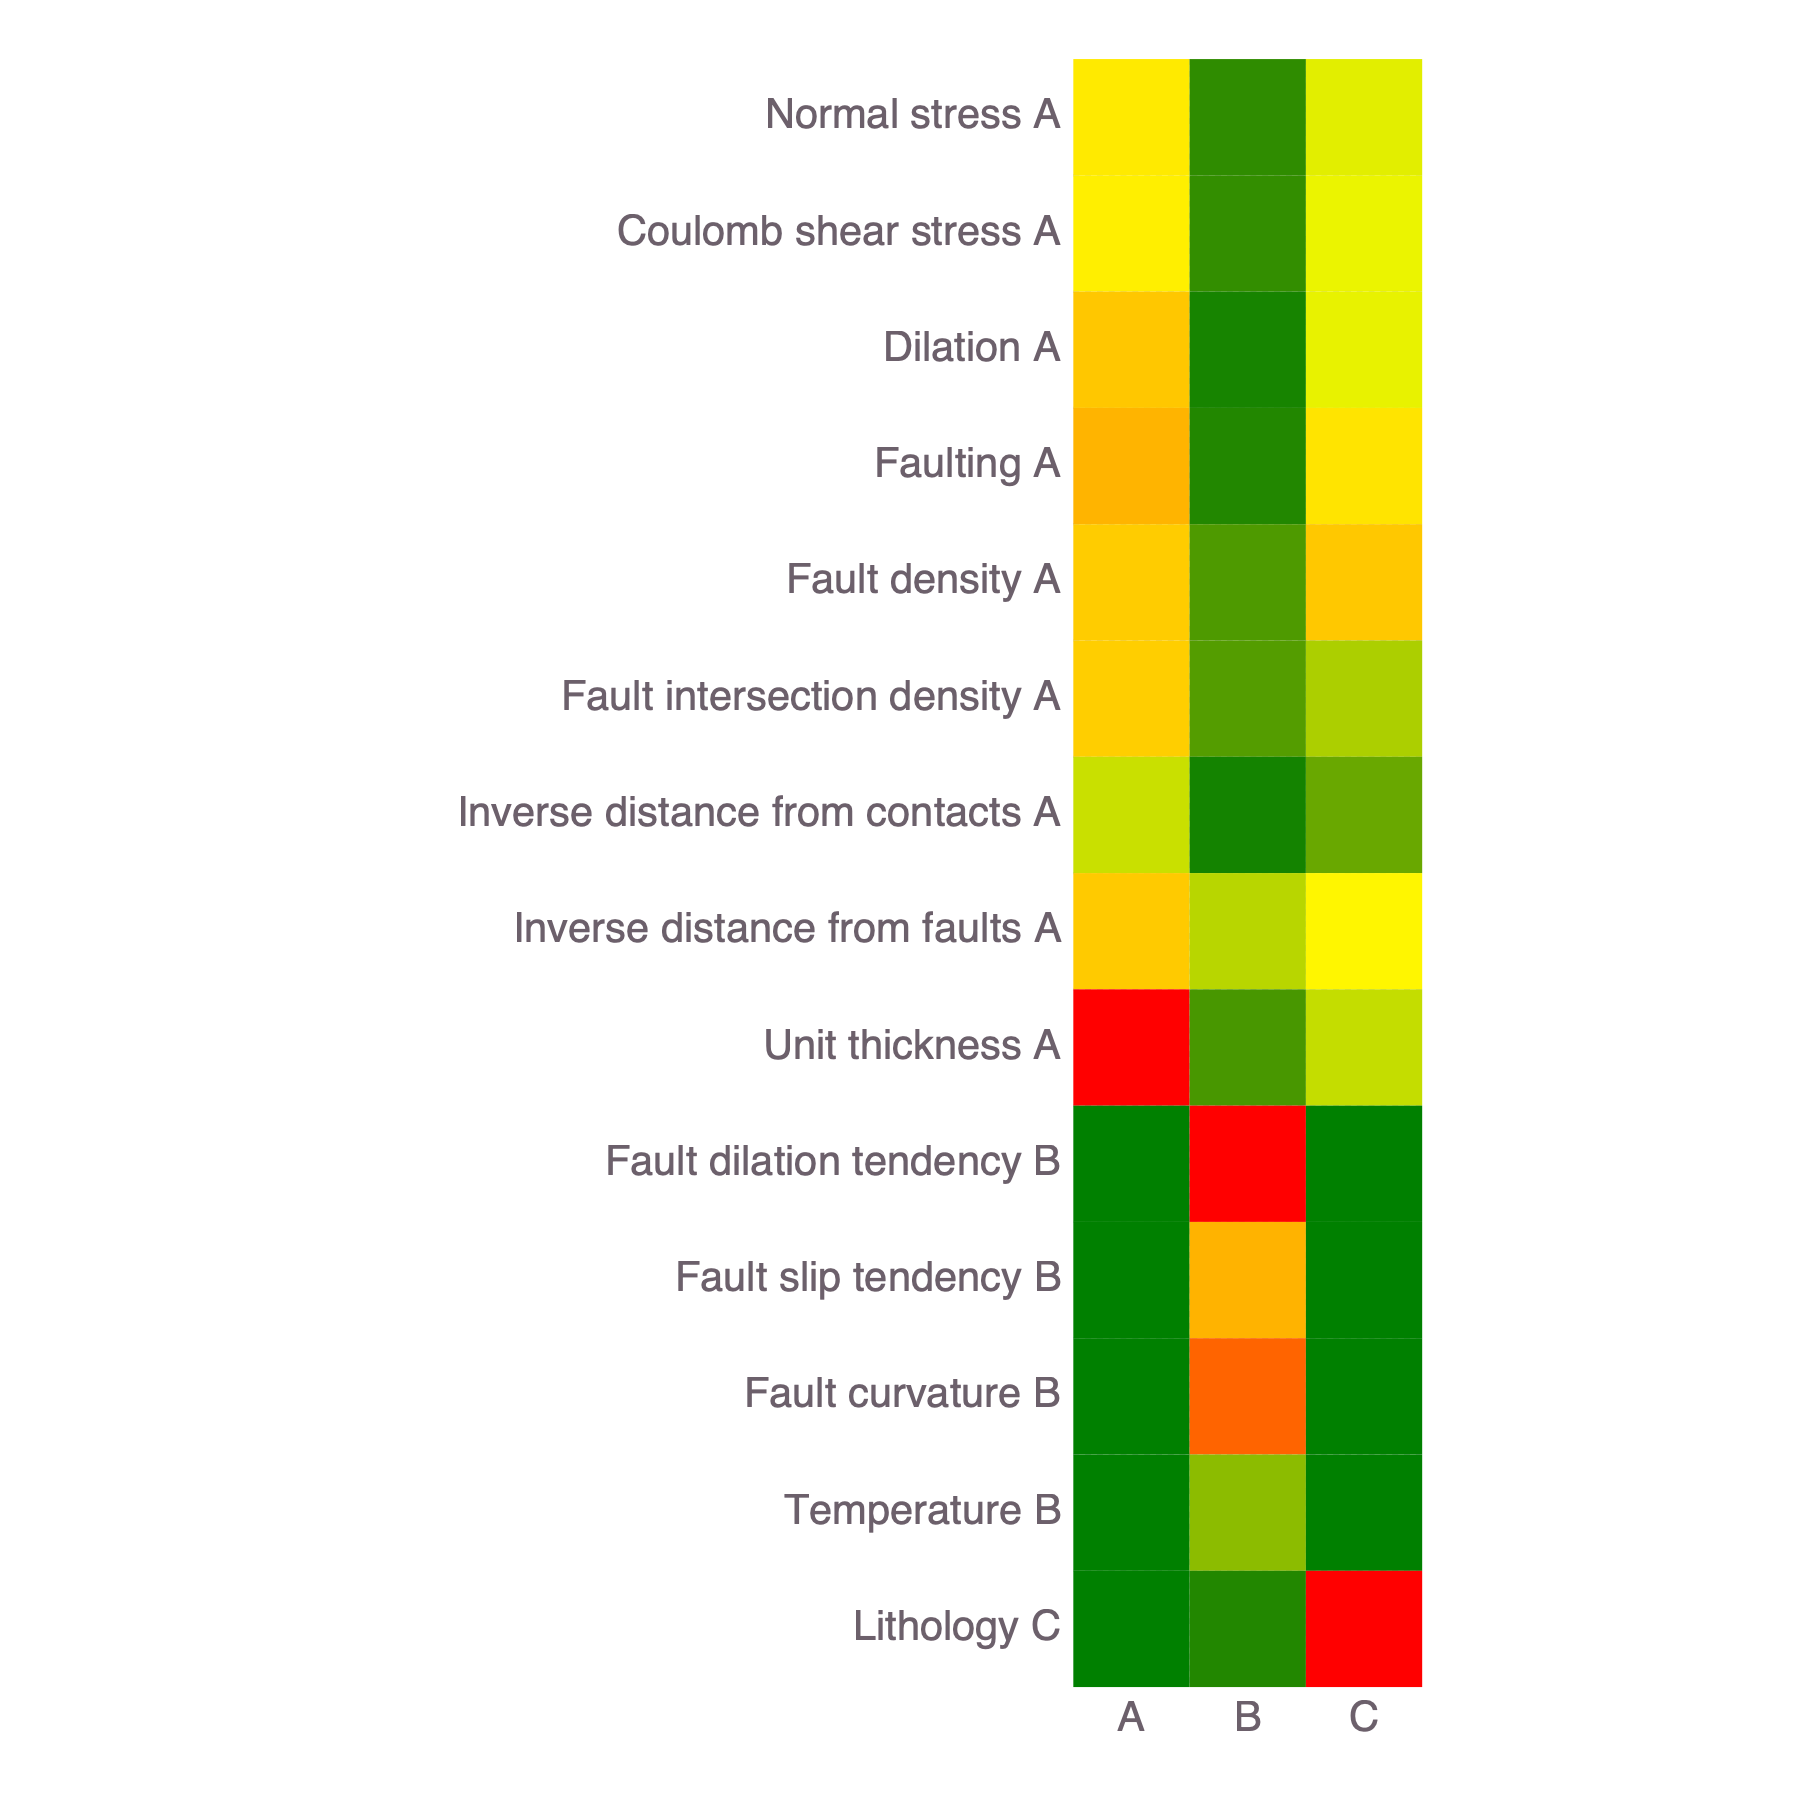
\includegraphics{../figures-set00-v9-inv-750-1000-dlan/attributes-3-labeled-sorted.png}
\caption{attributes-3-labeled-sorted}
\end{figure}

Note that the attribute matrix \texttt{W} is automatically modified to
account that a range of vertical depths is applied in characterizing the
site wells.

The well locations are also clustered into \textbf{3} groups:

This grouping is based on analyses of the location matrix \texttt{H}:

\begin{figure}
\centering
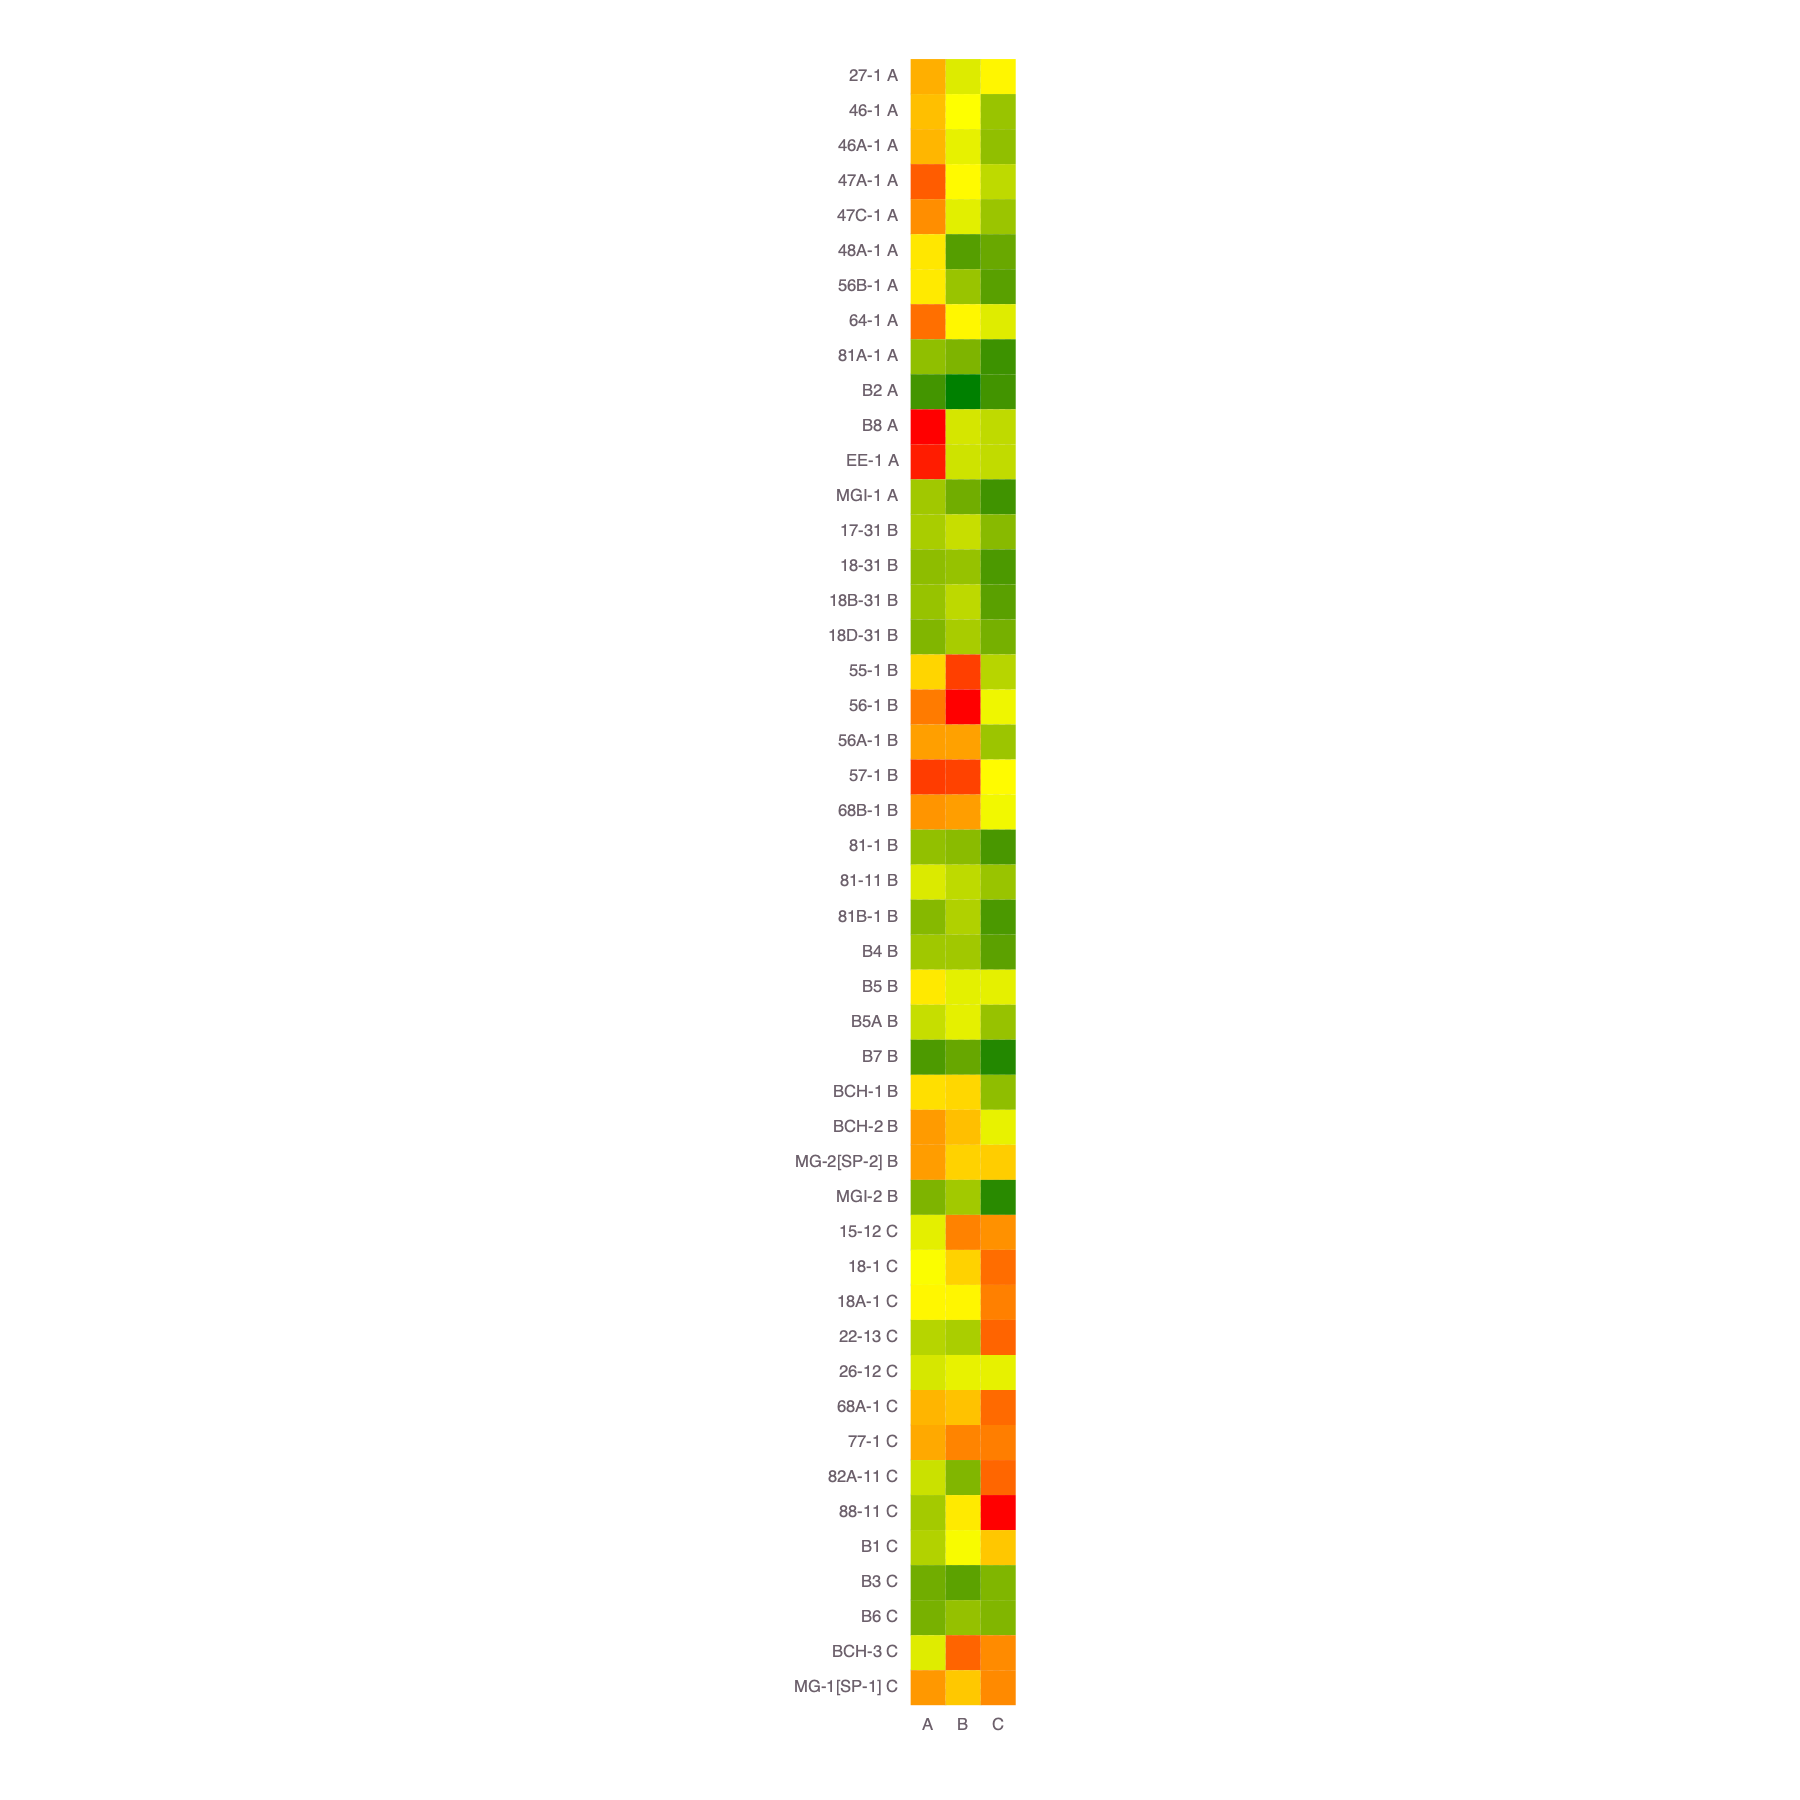
\includegraphics{../figures-set00-v9-inv-750-1000-dlan/locations-3-labeled-sorted.png}
\caption{locations-3-labeled-sorted}
\end{figure}

The map \url{../figures-set00-v9-inv-750-1000-dlan/locations-3-map.html}
provides interactive visualization of the extracted well location groups
(the html file can also be opened with any browser).

\begin{verbatim}
<iframe src="../figures-set00-v9-inv-750-1000-dlan/locations-3-map.html" frameborder="0" height="400" width="50%"></iframe>
\end{verbatim}


    % Add a bibliography block to the postdoc
    
    
    
\end{document}
